\chapter{Measurement of the \bsmumu effective lifetime}
\label{sec:lifetimemeasurement}

This chapter describes the measurement of the \bsmumu effective lifetime.% on 4.4~\fb of data.% on data that passes the selection requirements detailed in Chapter~\ref{selection_chapter}. 
Section~\ref{sec:fitstrategy} presents an overview of the analysis strategy used to measure the \bsmumu effective lifetime from data, the mass and decay time distributions of \bsmumu decays and backgrounds passing the selection described in Chapter~\ref{} must to known for the optimisation of the analysis strategy and the measurement of the effective lifetime. The \pdfs of the mass and decay time distributions are described in Sections~\ref{sec:ELmasspdfs} and~\ref{sec:DTpdfs} for signal and background decays. Due to the very rare nature of \bsmumu decays, the measurement strategy has been optimised to produce the lowest expected uncertainty on the measured \bsmumu effective lifetime these optimisation studies are detailed in Section~\ref{sec:toys}. Finally the measurement of the \bsmumu effective lifetime is presented in Section~\ref{sec:ELresults}.



%The overall fit strategy is described in Section~\ref{sec:fitstrategy} and greater detail of the components needed to make up the fit and the optimisation of the final configuration is given in the subsequent sections. The description of the mass and decay time \pdfs of \bmumu and background decays are given in Sections~\ref{sec:ELmasspdfs} and~\ref{sec:DTpdfs}. Toy studies are performed to optimise the final fit configuration, these studies are described in Section~\ref{sec:toys}. Finally the measurement of the \bsmumu effective lifetime is presented in Section~\ref{sec:ELresults}.
%{\it Probably need to give some more details here in order to set the scene for the sections better}


The work presented in this chapter was completed for this thesis except the areas where the same method as the branching fraction analysis is used. This includes the background mass \pdf evaluation and the expected signal and background yields for the data set, as well as the \bsjpisphi yields from data. 


\section{Analysis Strategy}
\label{sec:fitstrategy}
The effective lifetime is measured from the decay time distribution of bsmumu candidates passing the selection
However background decays also pass the selection
Therefore either need to know the pdfs that describe the backgrounds or use a way to separates the background from the signal so only the decay time distribution of the signal is left
Several methods were investigated to see which would perform best given the small number of expected events with 4.4 fb
The most successful method uses the sPlot method detailed in CITE
This provides a way to statically untangle signal and background distributions.
The EL is measured in 2 steps, 1st by performing a ml fit to the invariant mass, the fit is similar to the BF fit and the pdf includes components from the signal and backgrounds available in the data set. The mass fit measured the yields of the signal and background decays and compute sWeights for each decay depending on how signal-like or background-like the decay is. The weights are applied to the data set and the 2nd ml fit is performed to the signal weighted DT. In the fit only the signal DT pdf is needed because the backgrounds have been effectively removed. Due to the low statistics expected for the data set, Run 1 and Run 2 data are combined and the \ml fit to the mass and weighted decay time distributions are performed to the combined data.
The sWeights are given by … :(
A requirement of the sWeights only work if the mass and DT are not correlated. This has been check on signal and bkgnd decay and the correlation is negligible. Perhaps no table just the words?
The sPlot method is implemented using RooFit but there is a draw back in that we can’t use the weighted directly
This method is ideal because we know the mass pdfs from the BF but it’s hard to get the DT pdfs of the CBG.


The \bsmumu \el is measured from the decay time distribution of \bsmumu candidates passing the selection criteria described in Section~\ref{}. However the selection requirement do no completely separate real \bsmumu decays from the backgrounds, therefore to measure the \bsmumu effective lifetime either the \pdfs describing the decay time distribution of signal and backgrounds must be know or the background candidates must be removed from the data set leaving only the signal distribution. Several approaches were investigated to determine which would produce stable results for the measured \bsmumu effective lifetime on 4.4 \fb and yield the smallest expected statistical uncertainty on the result. The most successful approach uses the sPlot statistical method as described in~\cite{Pivk:2004ty} that provides a way to statistically untangle the signal and background distributions in a data set.

This method produces a two steps strategy to measure the \el. This first step is a unbinned \ml fit to the dimuon invariant mass spectrum, where components are included in the \pdf for \bsmumu decays and each background decay type. The mass fit measured the yields of the signal and background decays and from the fit sWeights are calculated for each component in the mass fit. The second step is to apply the sWeights of \bsmumu decays to the data set, effectively removed all background decays, and perform an unbinned \ml fit to the signal weighted decay time distribution to measure the \bsmumu \el. In the final fit only the \bsmumu decay time \pdf is needed to measure the \el. Due to the low statistics expected for the data set, Run 1 and Run 2 data are combined and the \ml fit to the mass and weighted decay time distributions are performed to the combined data.

%sWeights are calculated from the mass fit in the following way … and have the properties… they are optimised to give …

A requirement of the sPlot procedure is that the variable used to calculate the sWeights and the variable from which the observable is measured must be independent. The correlation of the mass and decay time of \bsmumu and the dominant background from \bbbarmumux decays has been evaluated using simulated decays and data. The correlation is of the order of a few percent, as shown in Table~\ref{tab:correlation}, therefore mass can be used to accurately determine sWeighted to me sure the \bsmumu effective lifetime.

\begin{table}[t!]
\begin{center}
\begin{tabular}{lcc}
\hline
Year & \bsmumu correlation &  \bbbarmumux correlation \\ \hline
2011 & -0.008  & 0.003  \\
2012 &  -0.006&   0.008\\
2015 &  -0.006&   0.010\\ 
2016 &  0.008& 0.002\\ \hline
\end{tabular}
\vspace{0.7cm}                                                                                                                                               
\caption{Correlation between mass and decay time for candidate from \bsmumu simulated decays and \bbbarmumux decays from data for 2011, 2012, 2015 and 2016 data taking conditions. The full effective lifetime selection is applied to simulated \bsmumu decays and \bbbarmumux decays in data must pass the effective lifetime selection requirements apart from the global BDT cut and have a dimuon invariant mass of 5447~\mevcc.}
\label{tab:correlation}
\end{center}
\vspace{-\baselineskip}%-2.7cm}                                                                                                                                               

\end{table}

The sWeights are calculated using the RooFit package~\cite{Verkerke:2003ir,}, however the raw sWeights from the mass fit cannot be used directly in the \ml fit to the decay time. The normalisation of the sWeights will not produce to correct statistical uncertainty on the effective lifetime measurement. Therefore the sWeights are re-normalised via
\begin{equation}
\omega^{'}_{i}= \omega_{i} \cdot \frac{\displaystyle\sum_{j} \omega{j}}{\displaystyle\sum_{j} \omega{j}^{2}}
\end{equation}
where $\omega_{i}$ are the sWeights values for each decays. The re-normalised sWeights will then produce the correct statistical uncertainty in a \ml fit to measure the \bsmumu effective lifetime.

The approach outlined here is studied to the measurement of the \bsmumu \el because the mass \pdfs are accurately known for the signal and background decays in the data set from the branching fraction analysis. Furthermore no knowledge is needed to the decay time \pdfs in the final fit, this is advantageous because decay time distribution of combinatorial background decays is challenging to accurately constrain. 
However the overall performance of this strategy depends on the \ml fit to the invariant mass distribution; how many background components are included in the fit and the mass range the fit covers. The determination of the final fit configuration was done using toy studies that are described in Section~\ref{sec:toys} that study a range of different mass ranges largest being 4900 - 6000 \mevcc. Therefore the development of the fit configuration requires the mass and decay time \pdfs of all background within the largest mass range need to be known as well as the signal \pdfs. 




\section{Mass \pdfs}
\label{sec:ELmasspdfs}
The selection criteria used to identify \bsmumu candidates for the \bmumu branching fraction and \bsmumu effective lifetime measurements are similar. 
The background decays passing the \bsmumu effective lifetime selection and in the mass range 4900 - 6000 \mevcc are the same as those passing the branching fraction selection, although the yields will be different.% due to the different particle identification requirements and the cut on the global BDT. 
Therefore the \ml fit to extract the sWeights is very similar to the fit to the mass distribution used to measure the \bmumu yields for the measurement of the \bmumu branching fractions. The \pdf used in the mass fit has the form
\begin{equation}
\mathcal{P}_{tot}(m) = N_{sig}\mathcal{P}_{sig}(m) + \displaystyle\sum_{i} N^i_{bkg}\mathcal{P}^i_{bkg}(m)
\end{equation}
where $i$ represents a particular background, $N_{sig(bkg)}$ are the signal (background) yields and $P_{sig(bkg)}$ are the signal (background) \pdfs. The background decays include; \bdmumu, \lambdab, \bdpimunu, \bsKmunu, \bpimumu, \bcjpsimunu and combinatorial background decays. For the effective lifetime measurement the \bdmumu decay is included as a background. 
%The same method is used to evalute the mass \pdfs as used for the mass \pfds used in the branching fraction measurement (Sect.~\ref{}). 


%The same shapes are used but the different particle identification and BDT requirements used in the selection are taken into account in the exact \pdfs used when relevant.

The \bsmumu and \bdmumu mass \pdfs are described by a Crystal ball functions, with the Run~1 parameters given in Table~\ref{tab:signalpdfRun1}. The Run~1 and Run~2 data sets are combined for the measurement of the \bsmumu \el therefore only one mass \pdf is needed to describe \bmumu decays in data. The choice of Run~1 or Run~2 parameters in the \pdf has a negligible affect on the measurement of the \bsmumu \el as shown in Section~\ref{}.

Mis-identified semi-leptonic decays, \lambdab, \bdpimunu, \bsKmunu, \bpimumu, \bcjpsimunu,  are described by Argus functions evaluated from simulated decays using the same method as described in Section~\ref{sec:backgrounds}. The effective lifetime particle identification requirements and the cut on the global BDT are taken into account in the evaluation of the \pdf shapes. In the same was as the mass \pdfs used for the measurement of the \bmumu branching fraction, \bdpimunu and \bsKmunu are modelled with one common \pdf and so are \bpimumu decays.

Backgrounds from mis-identified \bhh decays are described by the double crystal ball function evaluated using the method described in Section~\ref{sec:backgrounds} with the effective lifetime particle identification requirements applied. Finally the combinatorial background is modelled with a decaying exponential where the slope is left free to float in the final fit.

The mass \pdfs for the signal and backgrounds are evaluated for the mass range 4900 to 6000~\mevcc to be used in the toy studies described in Section~\ref{sec:toys}. The parameters used describing the background shapes are given in Appendix~\ref{}.

{\it Is what I have said about the background pdfs correct? If the PID and BDT are not taken into account, then I can say that these cause a negligible change (though I assume BDT is taken into account to the semi-leptonic backgrounds!} and they are only used in the toys to the description does not need to be perfect. Simple to get around!}

\section{Decay time \pdfs}
\label{sec:DTpdfs}
%Start clearly explain the bias on the decay time pdf and this effects signal and background
The efficiency of the selection criteria to identity candidates for the measurement of the \bsmumu \el varies as a function of decay time for both signal and background decays, biasing the decay time distribution. The bias arises because variables used in the selection and the global BDT, such as the isolations and the B meson impact parameter and flight distance significance, are correlated with the decay time. Consequently cuts placed on these variables have a non-uniform efficiency across the decay time range. Therefore the \pdf describing the decay time changes from a decaying exponential to
\begin{equation}
\mathcal{P}(t) = \epsilon(t) \times e^{-t/\tau}
\end{equation}
where $\epsilon(t)$ is the selection efficiency as a function of decay time. 
The decay time distribution and selection efficiency as a function of decay time are shown in Figure~\ref{fig:accpteg} for simulated \bsmumu decays at different stages through the selection. The cut on the global BDT causes the biggest decay time bias as expected since it is the hardest selection cut applied. The decay time distributions for the semi-leptonic and \bhh decays are not shown because there are too few decays left after the selection.

To measure the \bsmumu effective lifetime the efficiency of the selection on \bsmumu decay as a function of decay time must be accurately modelled. The determination of $\epsilon(t)$ for \bsmumu decays is described in Section~\ref{sec:signalDTpdf}. Although the weighting procedure used to measure the \bsmumu effective lifetime means that the decay time \pdfs of the backgrounds present in the data set are not needed, realistic  descriptions of these decay time \pdfs are necessary for the to studies used to determine the optimal fit configuration. The background \pdfs are used described in Section~\ref{sec:bkgDTpdf}.
% I need to say somewhere what the lifetime used to generate the decay time pdf for \bsmumu decays is.

\begin{figure}[htbp]
    \centering
   \begin{subfigure}[b]{0.48\textwidth}
        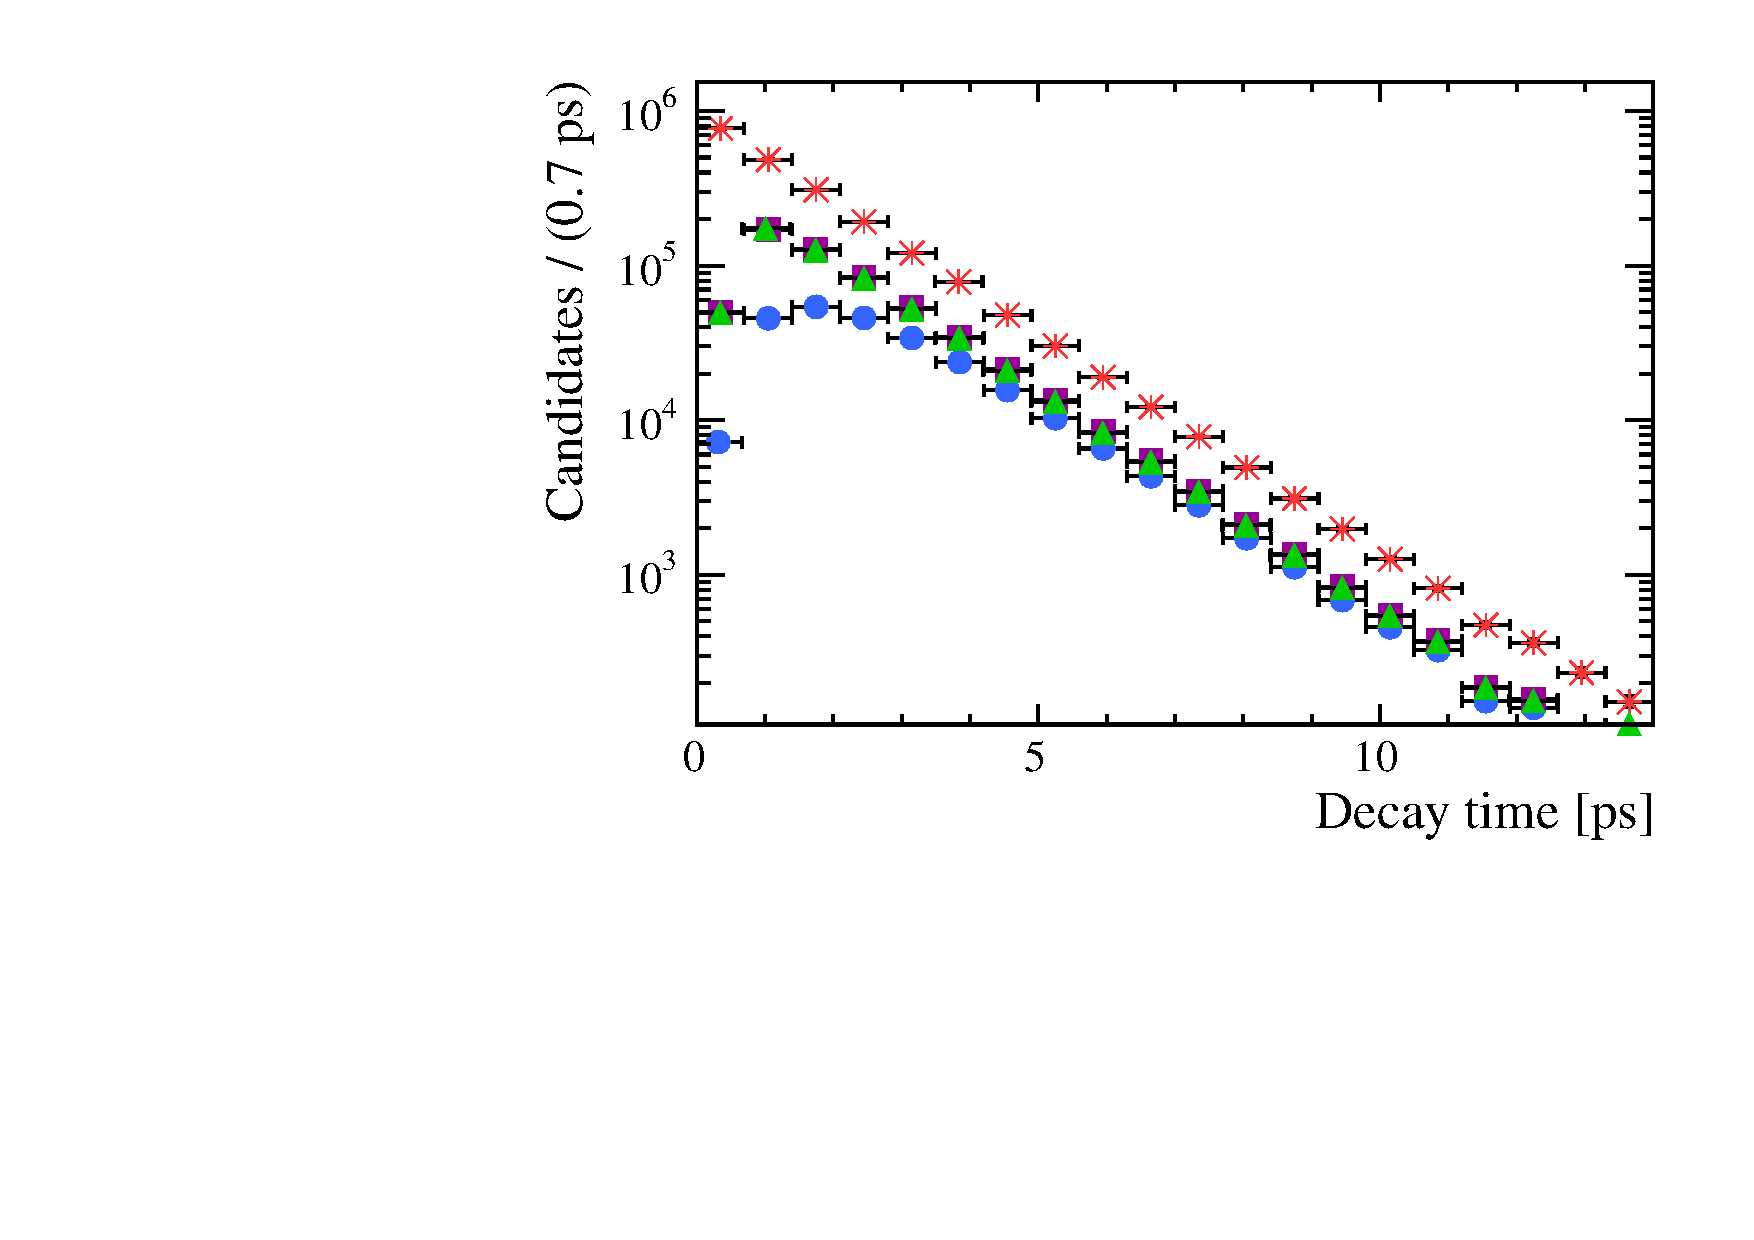
\includegraphics[width= \textwidth]{./Figs/LifetimeMeasurement/DT.pdf}
        %\caption{ }                                                                                                                    
        %\label{fig:BDTSsig}                                                                                                            
    \end{subfigure}
   ~ %add desired spacing between images, e. g. ~, \quad, \qquad, \hfill etc.                                                         
      %(or a blank line to force the subfigure onto a new line)                                                                         
    \begin{subfigure}[b]{0.48\textwidth}
       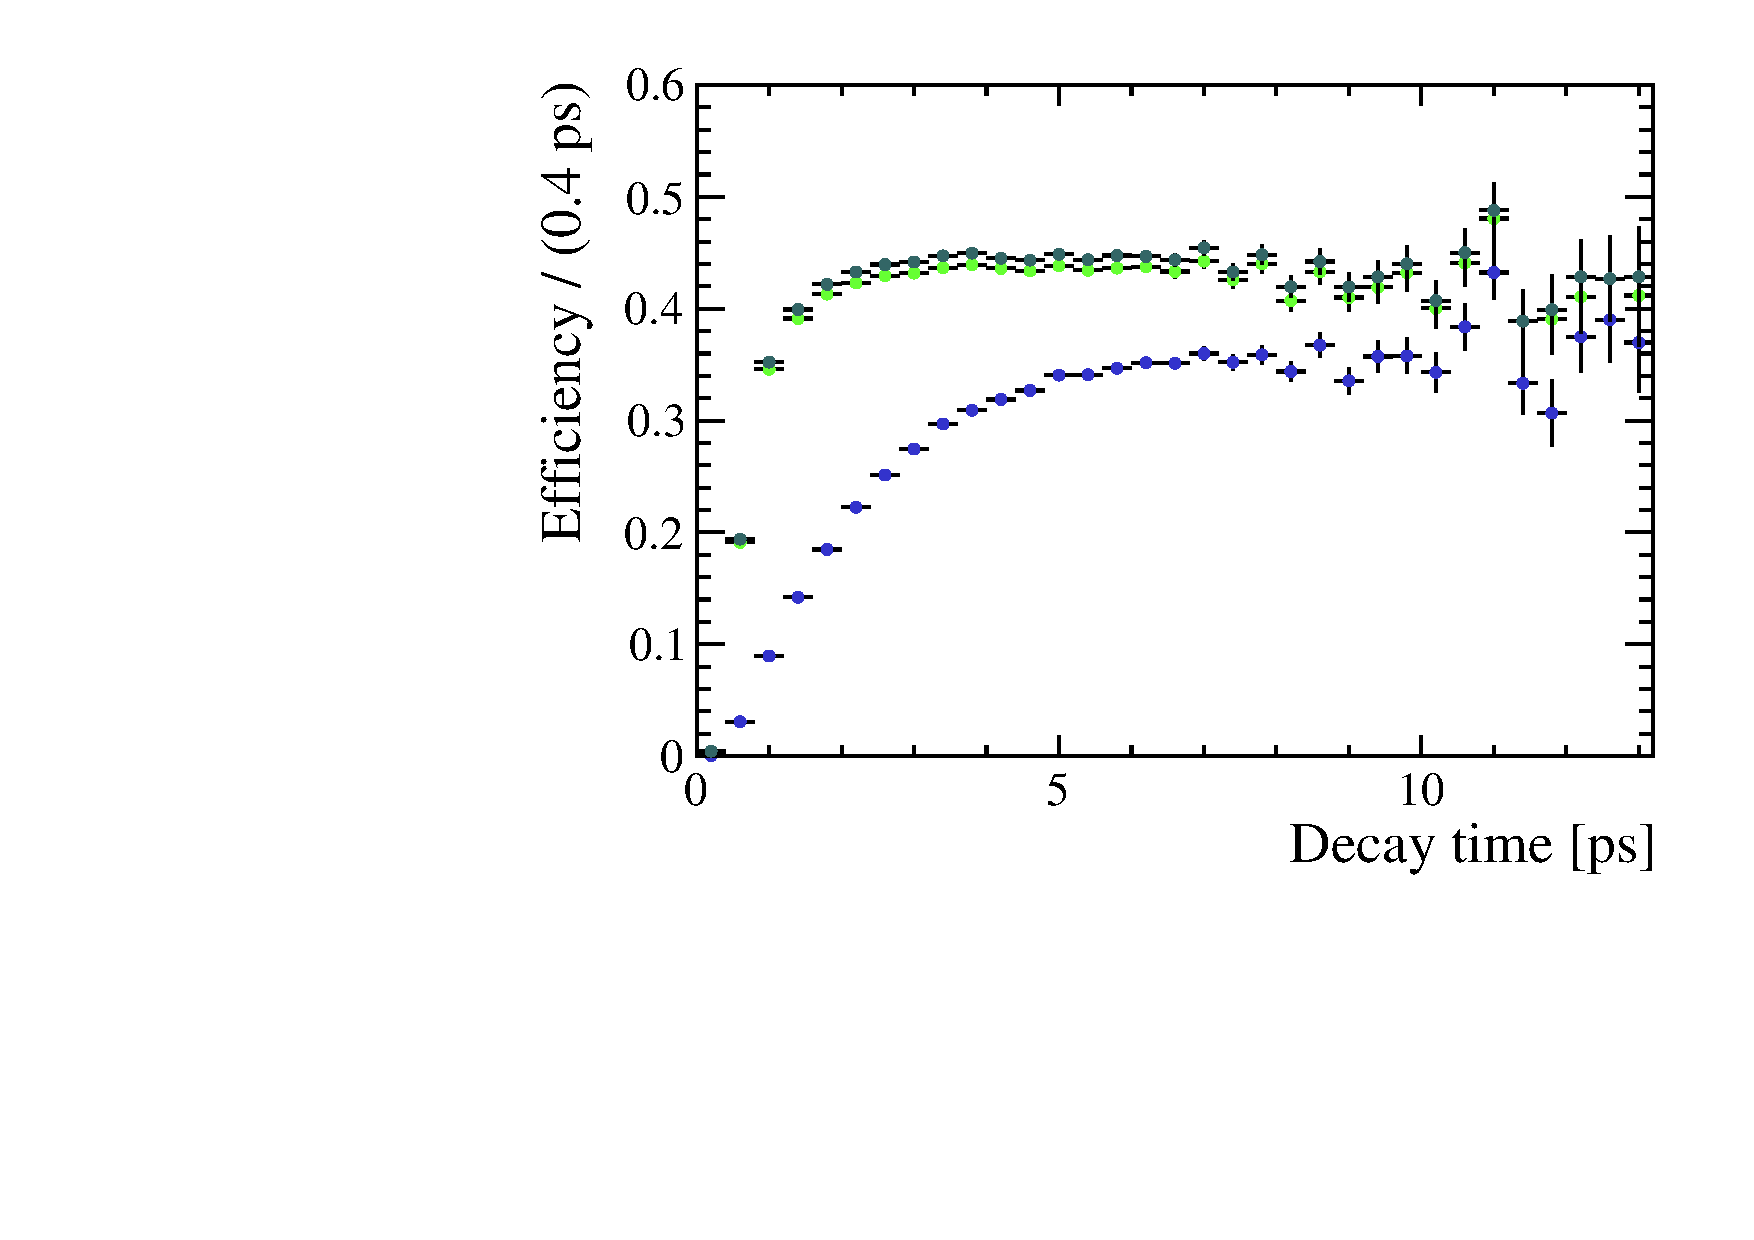
\includegraphics[width=\textwidth]{./Figs/LifetimeMeasurement/Accpt.pdf}
      %  \caption{ }                                                                                                                    
     %   \label{fig:BDTSbkg}                                                                                                            
   \end{subfigure}
    \caption{Decay time distribution (left) and selection efficiency as a function of decay time (right) for 2012 \bsmumu simulated decays at different different stages of the selection process. The decay time distributions and efficiencies are shown for reconstructed decays that pass the trigger, stripping and pre-selection cuts (turquoise), the decays that go on to pass PID requirements (green) and decays that pass all selection requirement including the global BDT cut (blue). Also the decay time distribution is shown for all generated simulated decays (purple).} %Hmm can’t see them all on the decay time dist! Perhaps separate trigger or add in more MC?
    \label{fig:accpteg}
\end{figure}

\subsection{\bsmumu decay time pdf}
\label{sec:signalDTpdf}
The selection efficiency of \bsmumu decays as a function of decay time is modelled by an `acceptance' function. A range of different models were investigated for the acceptance function, the parameterised acceptance 
\begin{equation}
\epsilon(t) = \frac{[a(t - t_{0}]^{n}}{1 + a(t - t_{0}]^{n}}
\label{eq:accpt}
\end{equation}
used in~\cite{} was found be describe the \bsmumu decay time efficiency best. The acceptance function parameters are taken from a fit to simulated \bsmumu decays and are fixed in the fit to data. The parameters could not be determined from data because there are too few \bsmumu decays in data and the efficiency distribution of the more abundant \bhh decays after the selection is quite different to that of \bsmumu. 


In general simulated decays model distributions in data reasonably well, however the number of tracks present in an event are not well modelled in the simulation. %The isolation variables used in the global BDT depend on the number of track in an event and the isolation variables are also correlated with the decay time of the \bs. 
Although the \bsmumu decay time distribution does not itself depend on the number of tracks present in the event, the isolations used in the global BDT do. Therefore the selection efficiency as a function of decay time depends on the number of tracks in the event and cannot be accurately described by simulated decays alone. To overcome this the number of tracks in an event for simulated \bsmumu decays are weighted using information from the number of tracks per event for \bdkpi decays in both data and simulation. 

The selection requirements listed in Table~\ref{} are used to identify \bdkpi decays in data and simulated decays but importantly the global BDT cut is not applied. The DLL$_{K\pi}$ variable is used to separate \bdkpi decays from other \bhh decays in data and the loose trigger requirements used for the branching fraction analysis are applied to data and simulated decays to keep a high trigger efficiency\footnote{The Hlt2Phys Dec trigger decision was not correctly implemented in 2016 simulated decays, therefore the DEC decisions of a combination of trigger lines designed to select \bhh are used to emulate the Hlt2Phys DEC trigger decision. The trigger lines are Hlt2Topo2BodyDecision, Hlt2B2HH\_Lb2PPiDecision, Hlt2B2HH\_Lb2PKDecision Dec, Hlt2B2HH\_B2PiPiDecision, Hlt2B2HH\_B2PiKDecision, Hlt2B2HH\_B2KKDecision and Hlt2B2HH\_B2HHDecision. These trigger lines are applied to both data and simulated decays.}. The same requirements are applied to simulated decays. The distribution of the number of tracks present in events containing \bdkpi decays is obtained from data by performing a maximum likelihood fit to the \bd mass distribution and extracting sWeights. The distribution of the number of tracks per events is compared for simulated \bdkpi decays and sWeighted \bdkpi decays in data. The mass fits to \bdkpi decays in data are shown in Figure~\ref{fig:ntracksmassifts} and the normalised distributions of the number of tracks per event in data and simulated decays is shown in Figure~\ref{fig:nTracksMCDataComp}. Each year of data taking is kept separate and the same simulation version is used for \bdkpi simulated decays as available for \bsmumu decays.



\begin{figure}[ht]
  \centering
    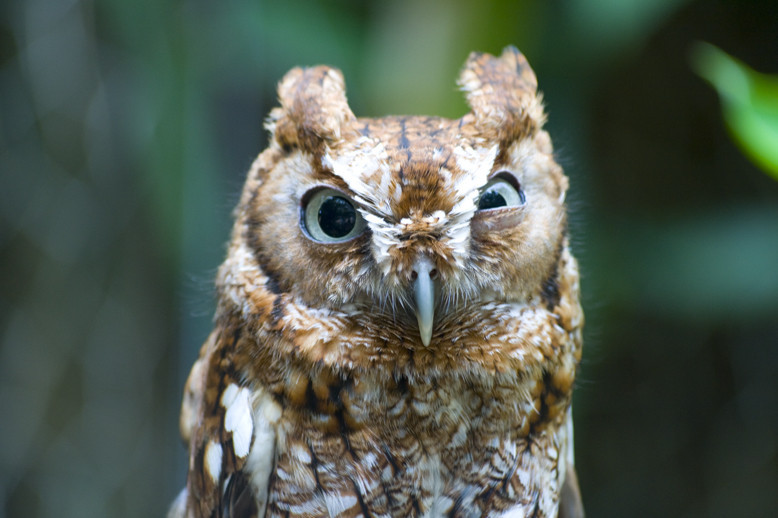
\includegraphics[width=0.4\textwidth]{./Figs/placeholder.jpeg}
    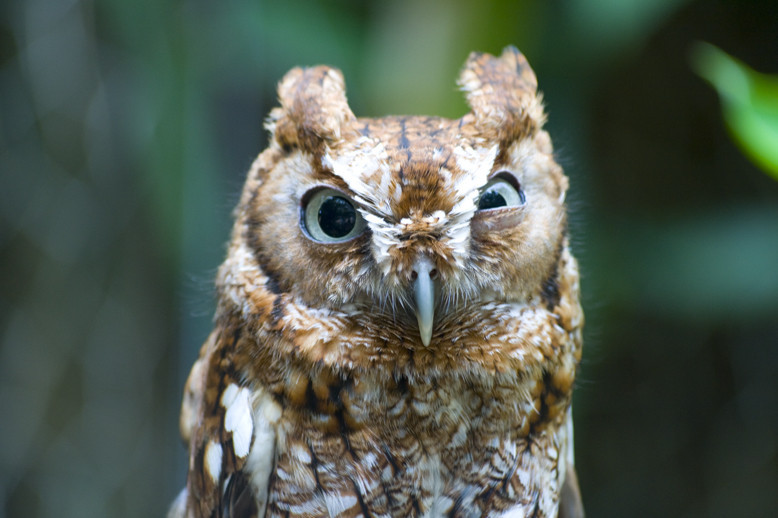
\includegraphics[width=0.4\textwidth]{./Figs/placeholder.jpeg}
    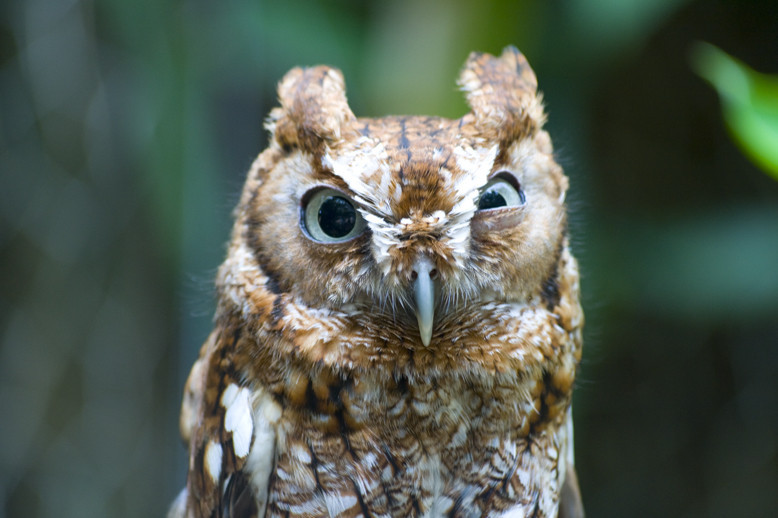
\includegraphics[width=0.4\textwidth]{./Figs/placeholder.jpeg}
    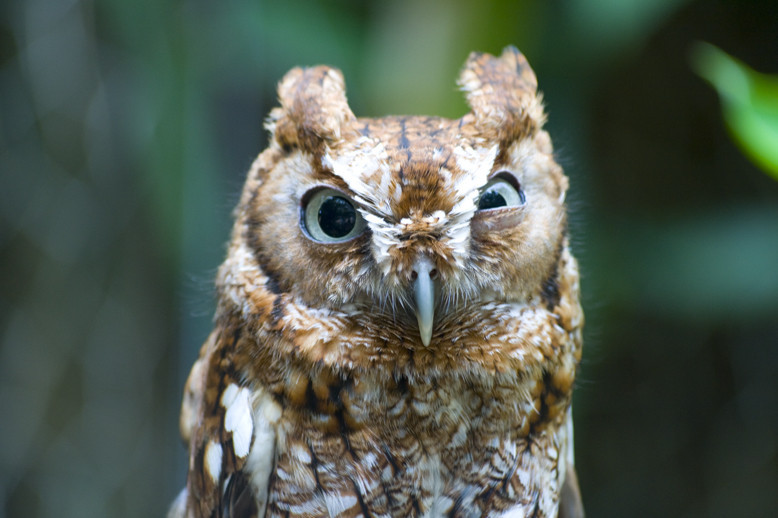
\includegraphics[width=0.4\textwidth]{./Figs/placeholder.jpeg}
  \caption{Mass fits to \bdkpi data for each each to find the sWeights to get the number of tracks per event for \bdkpi decays.}
  \label{fig:ntracksmassifts}
\end{figure}
\FloatBarrier


\begin{figure}[ht]
  \centering
    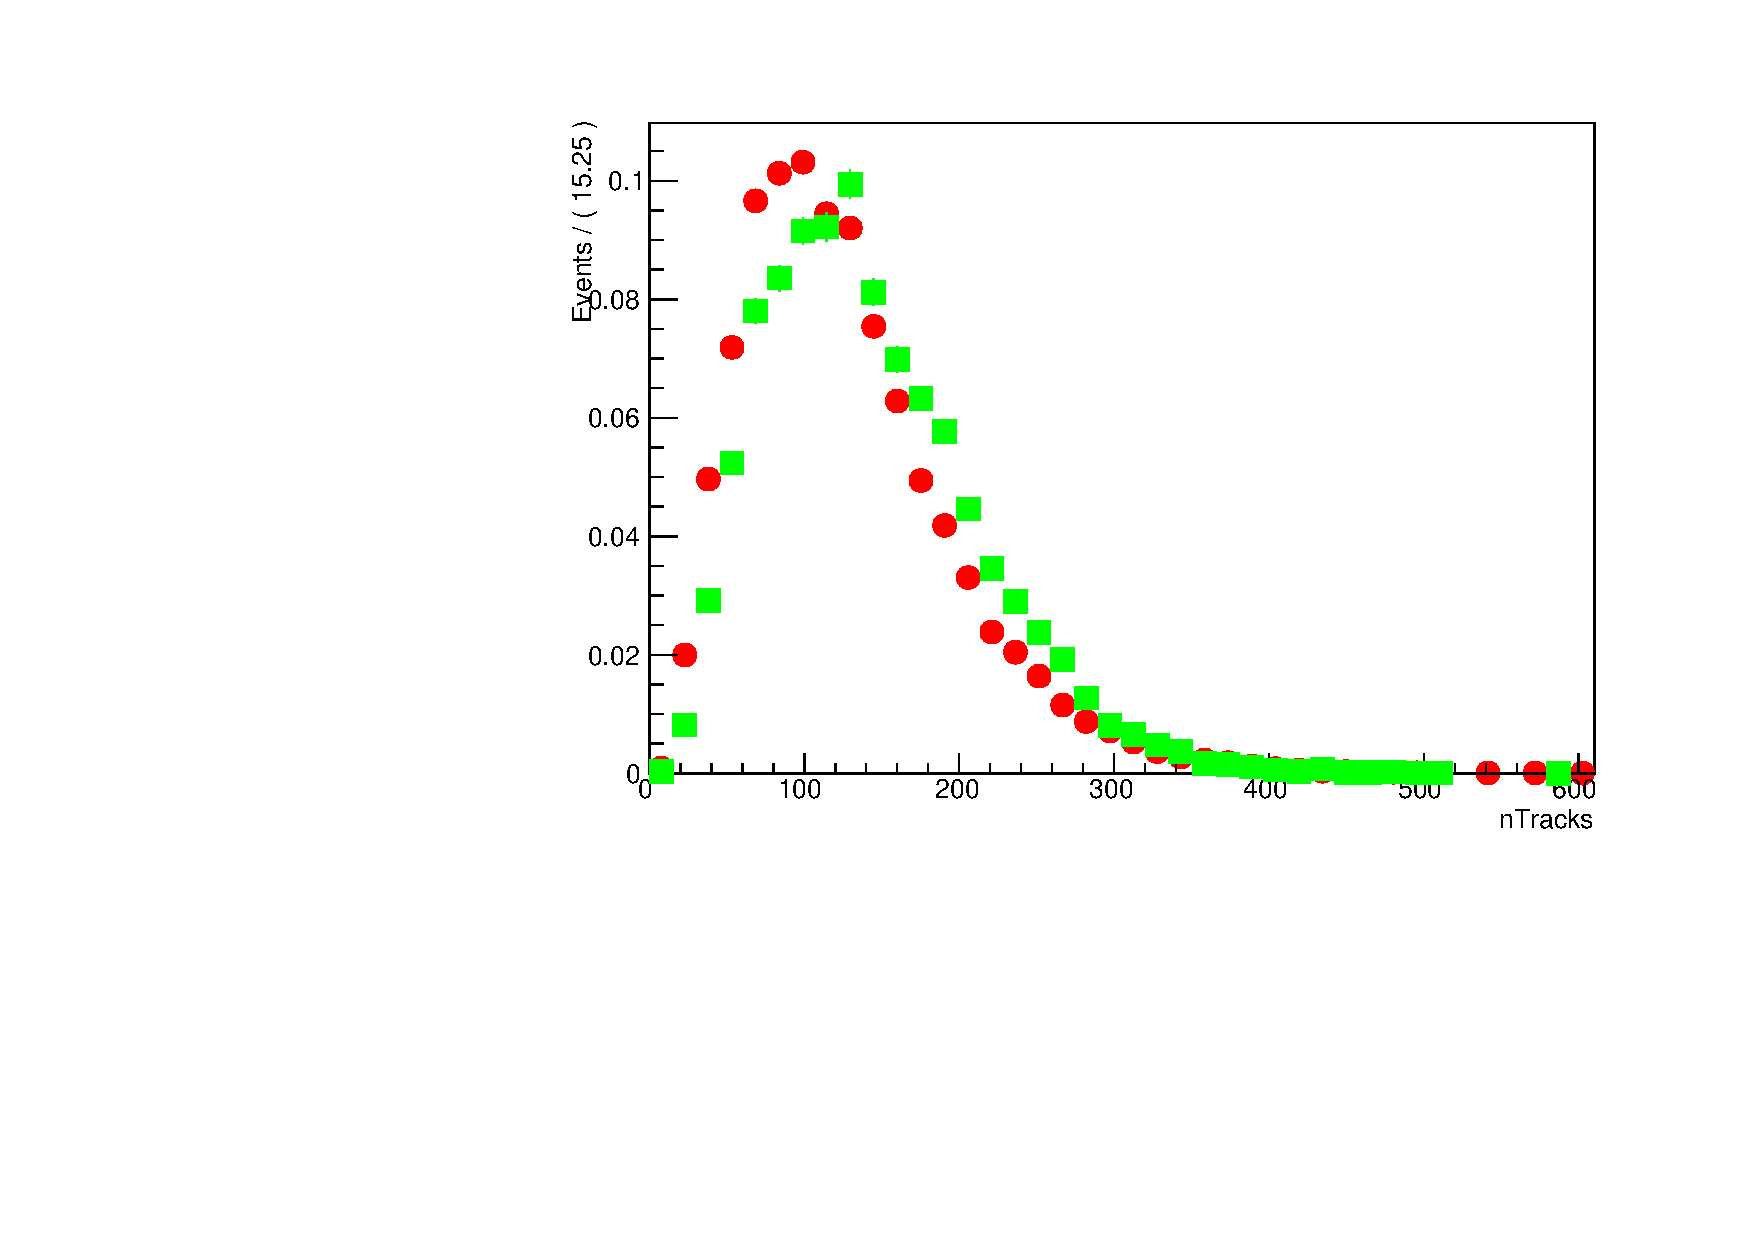
\includegraphics[width=0.4\textwidth]{./Figs/LifetimeMeasurement/2011_nTracks_Bd2KPi_MC_data_comparison_Dec_triggers.pdf}
    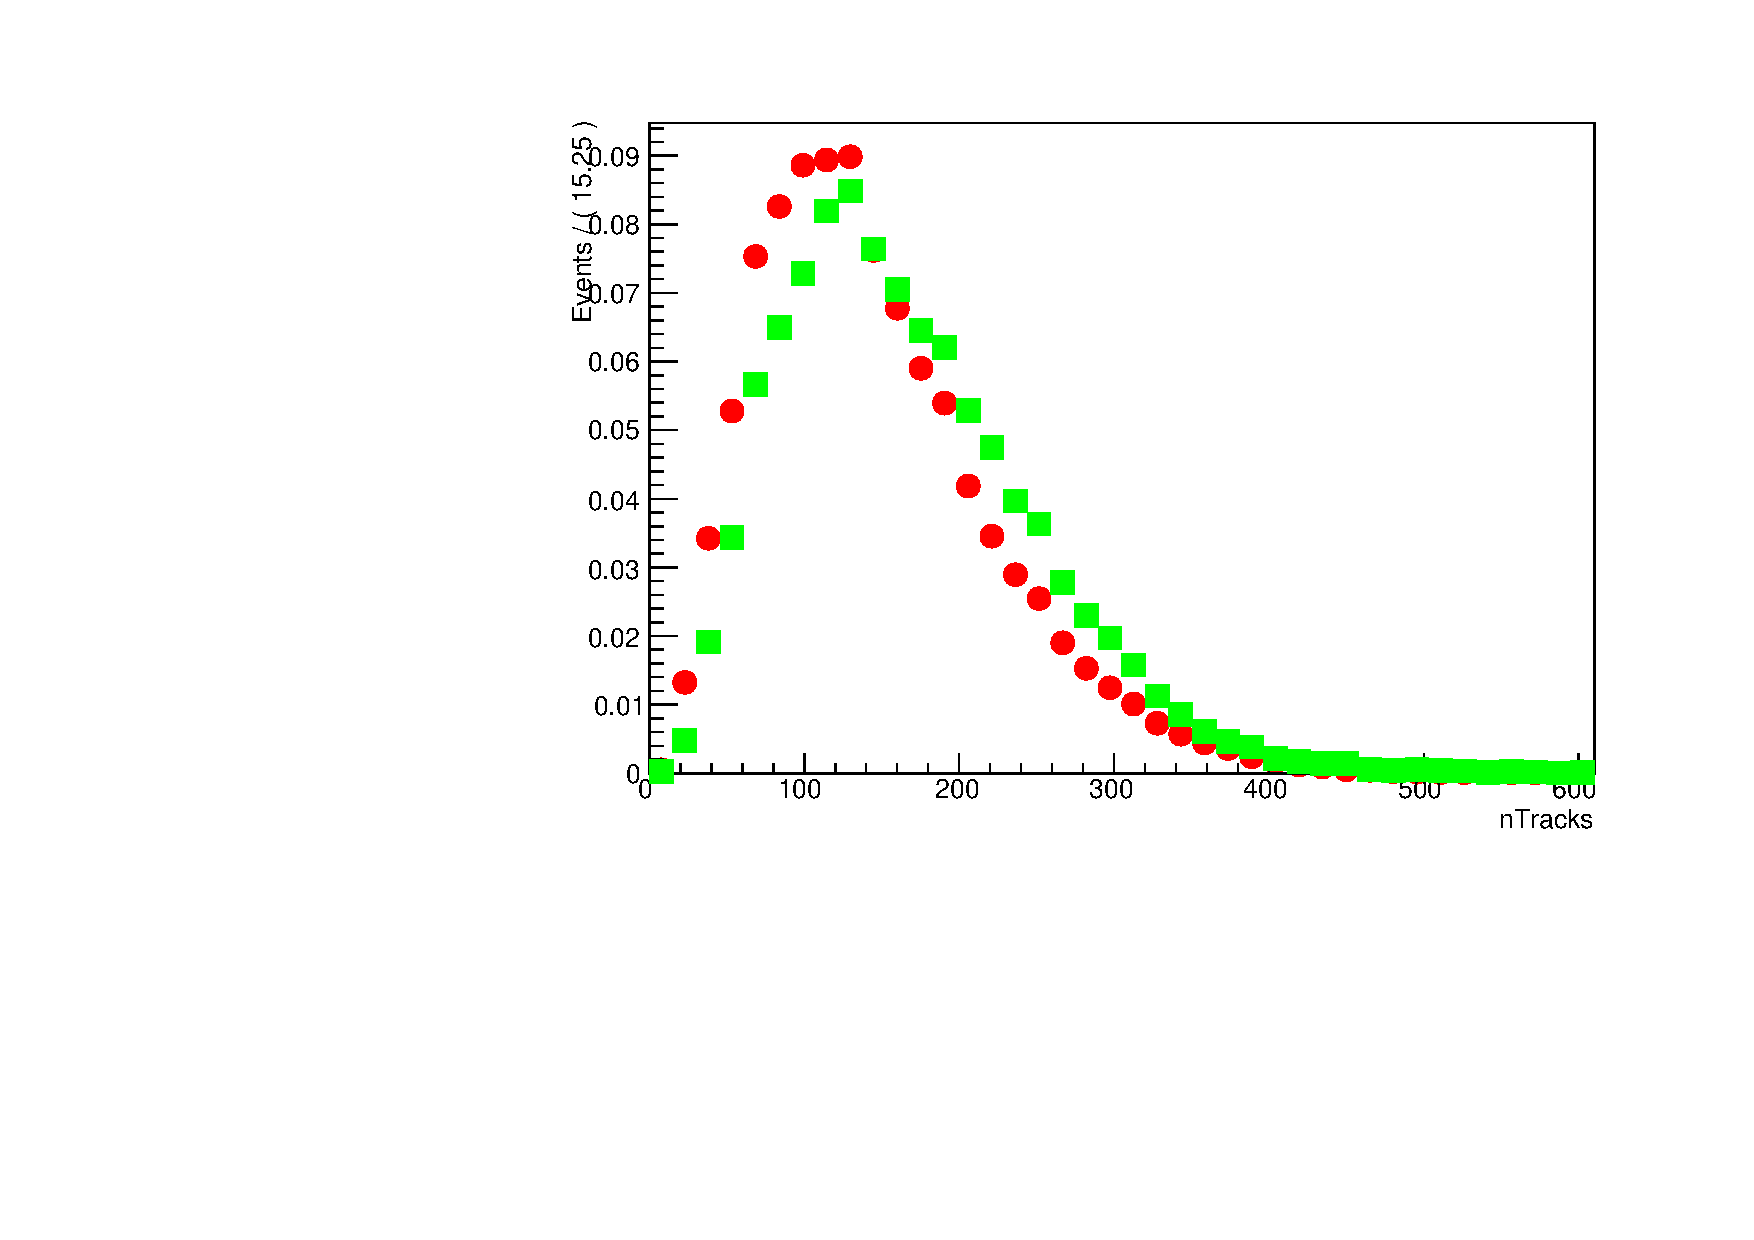
\includegraphics[width=0.4\textwidth]{./Figs/LifetimeMeasurement/2012_nTracks_Bd2KPi_MC_data_comparison_Dec_triggers.pdf}
    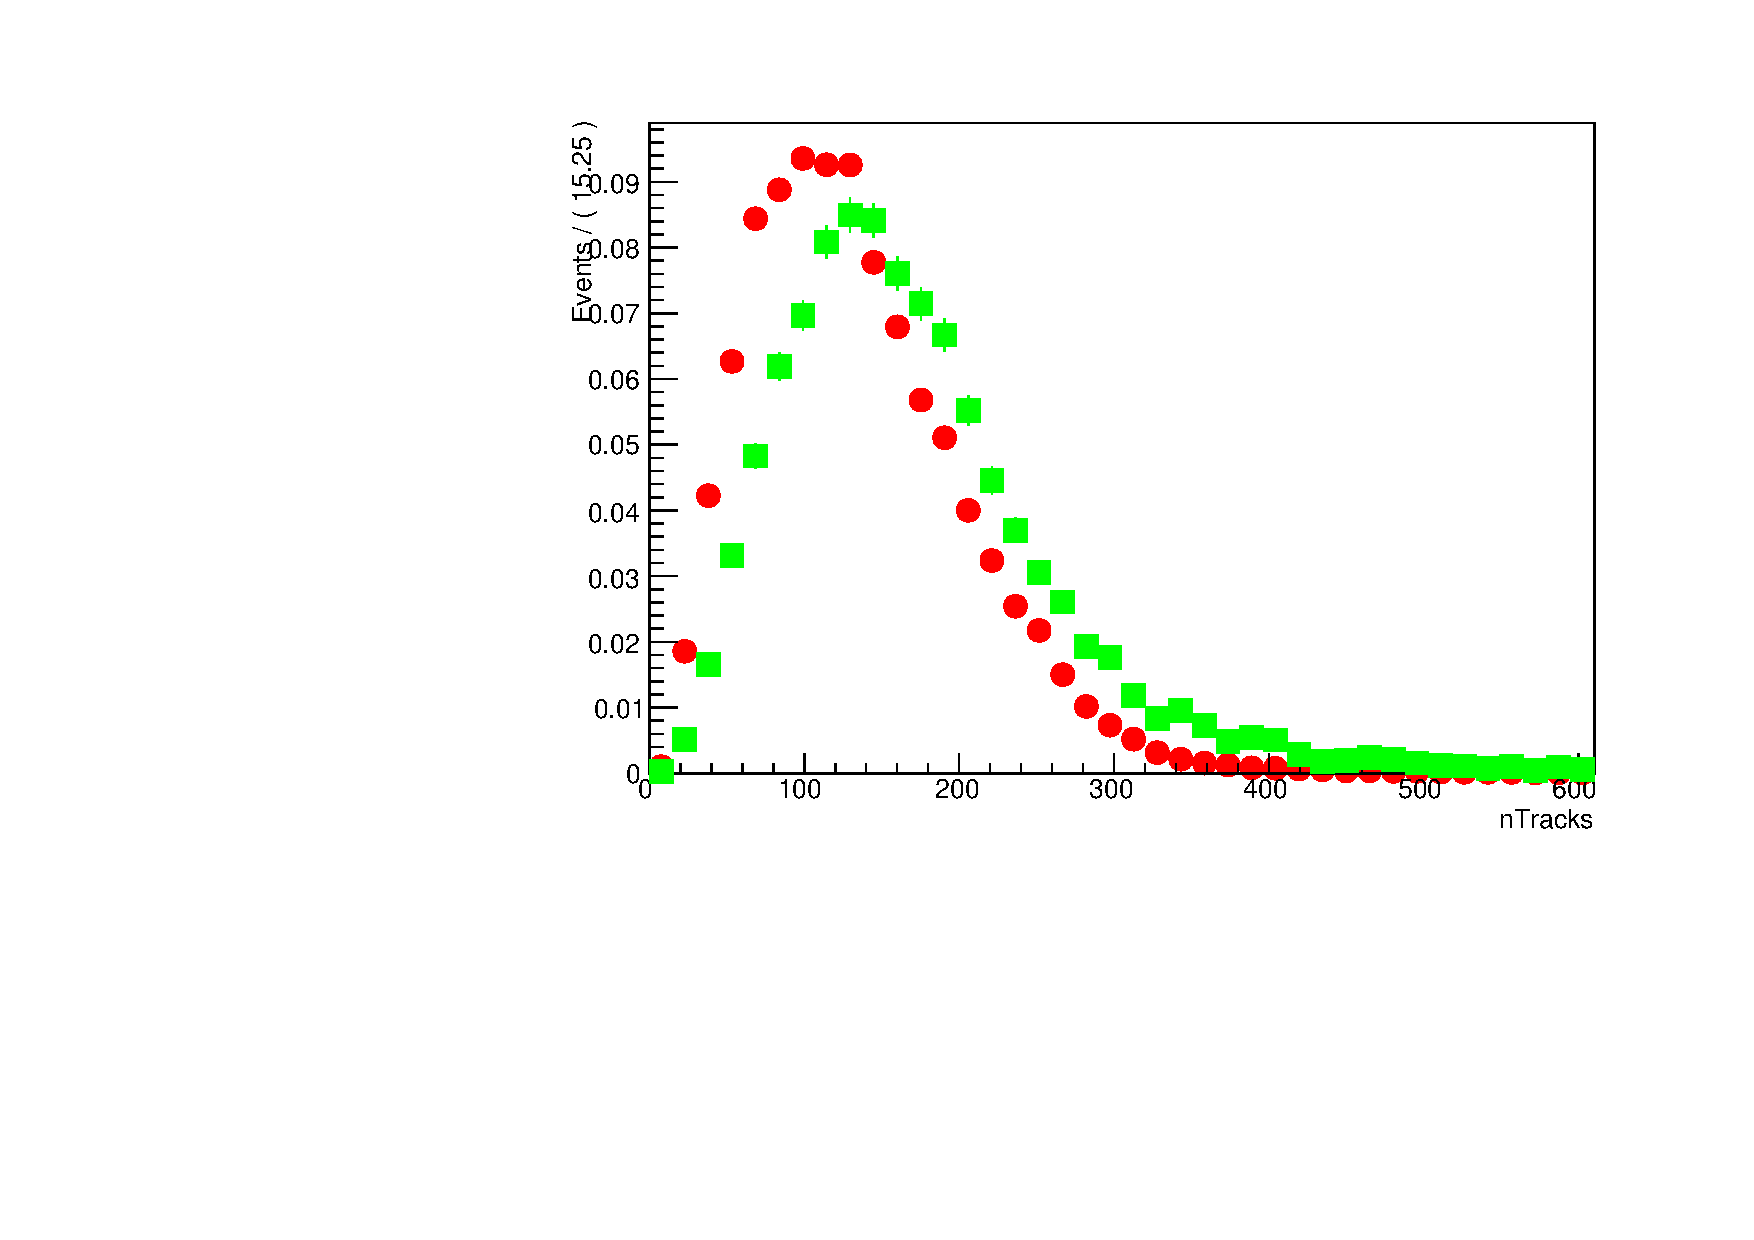
\includegraphics[width=0.4\textwidth]{./Figs/LifetimeMeasurement/2015_nTracks_Bd2KPi_MC_data_comparison_Dec_triggers.pdf}
    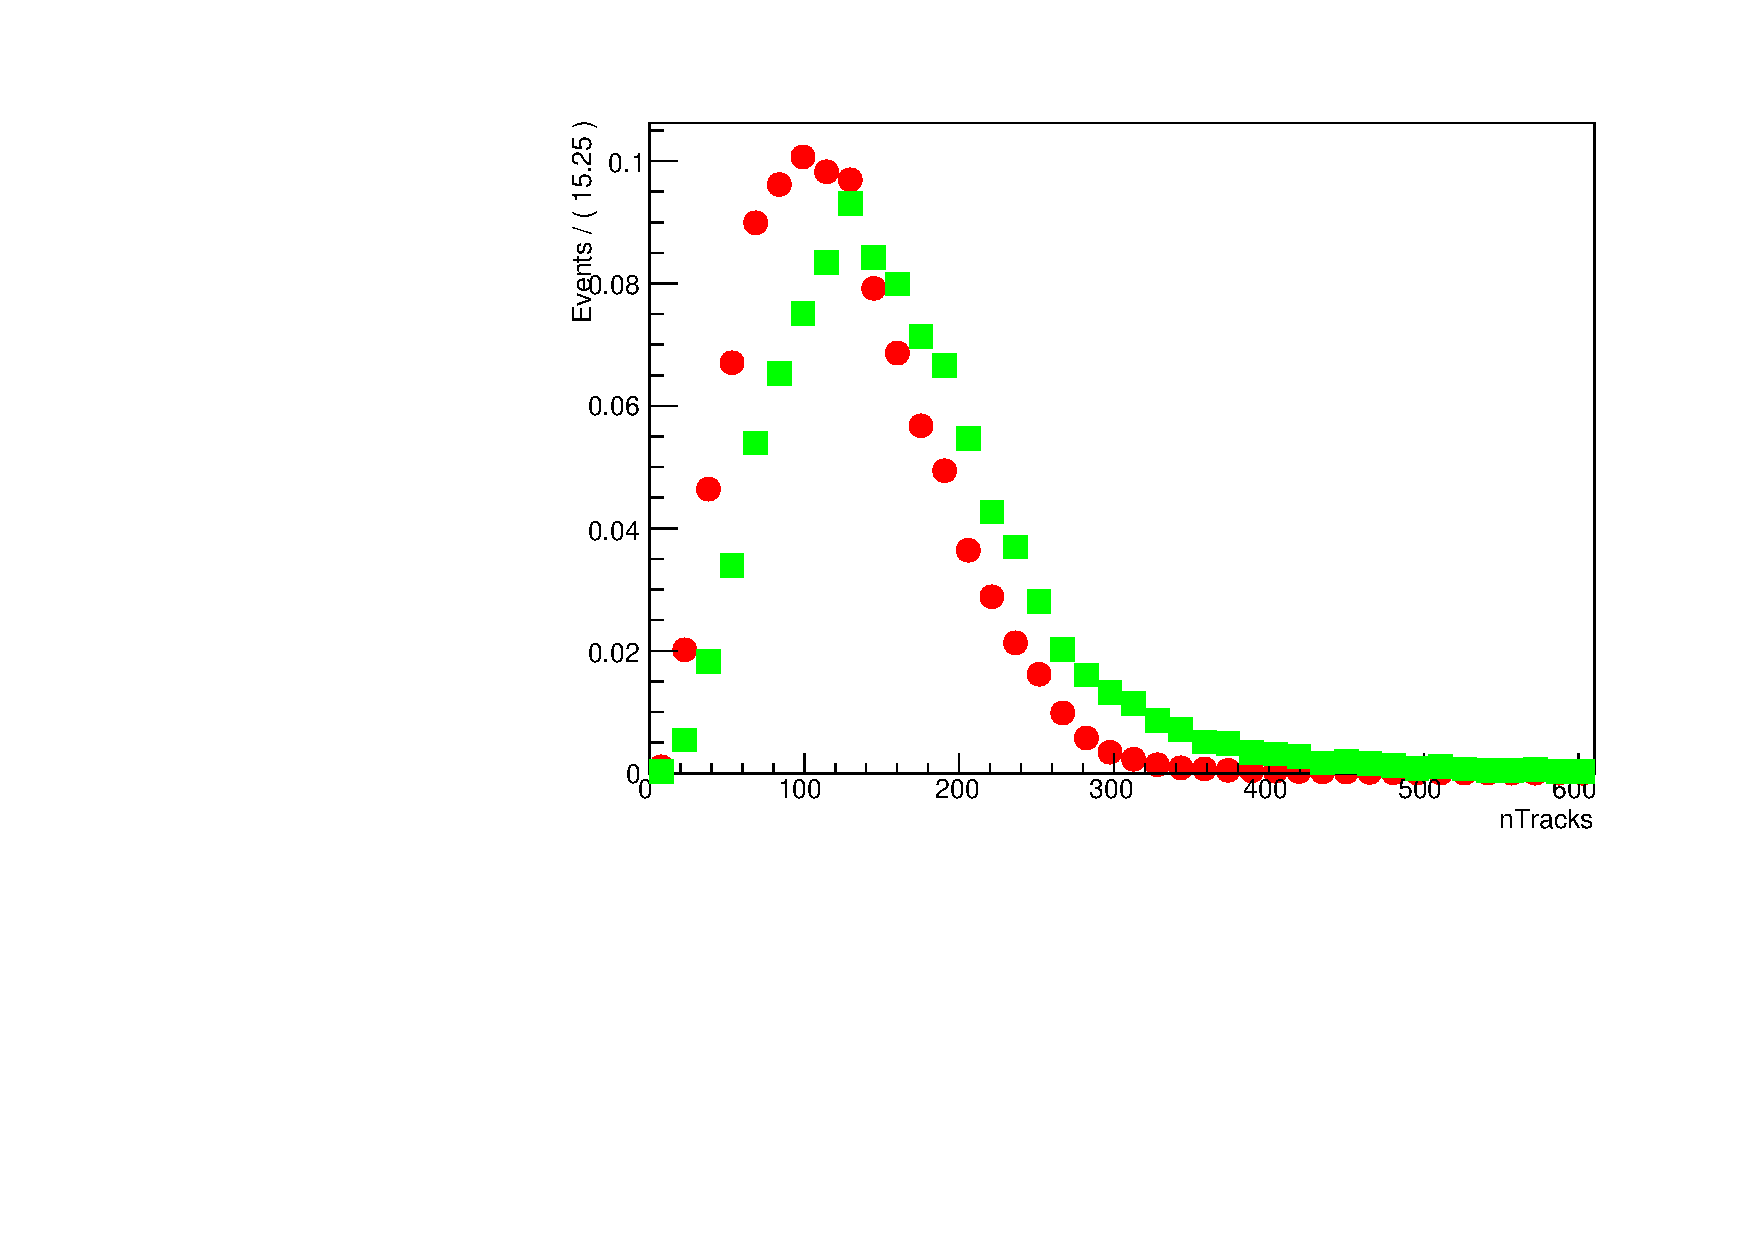
\includegraphics[width=0.4\textwidth]{./Figs/LifetimeMeasurement/2016_nTracks_Bd2KPi_MC_data_comparison_Dec_triggers.pdf}
  \caption{The number of tracks for \bdkpi candidates for 2011 (top left), 2012 (top right), 2015 (bottom left) and 2016 (bottom right), for Monte Carlo simulated events (red circles) and sWeighted data (green triangles). The histograms have been normalised to have unit area and so the y axis scale is arbitrary.}
  \label{fig:nTracksMCDataComp}
\end{figure}
\FloatBarrier


The distributions of the number of tracks per event for \bdkpi decays in data and simulated decays are used to weight the \bdkpi decays so that the distribution in simulation matches that in data. The weights are evaluated by taking the ratio of the normalised histograms in Figure~\ref{fig:nTracksMCDataComp} for the number of tracks per event in data and simulation for each year. The affect on the decay time distribution of using these weights and then applying the global BDT cut is shown in Figure~\ref{fig:BdToKpi_weightDecayTime} for the simulated \bdkpi decays. The different between the decay time distributions with and without the weights is not large but clearly noticeable at low decay times where the change in selection efficiency is greatest. 

\begin{figure}[htbp]
  \centering
    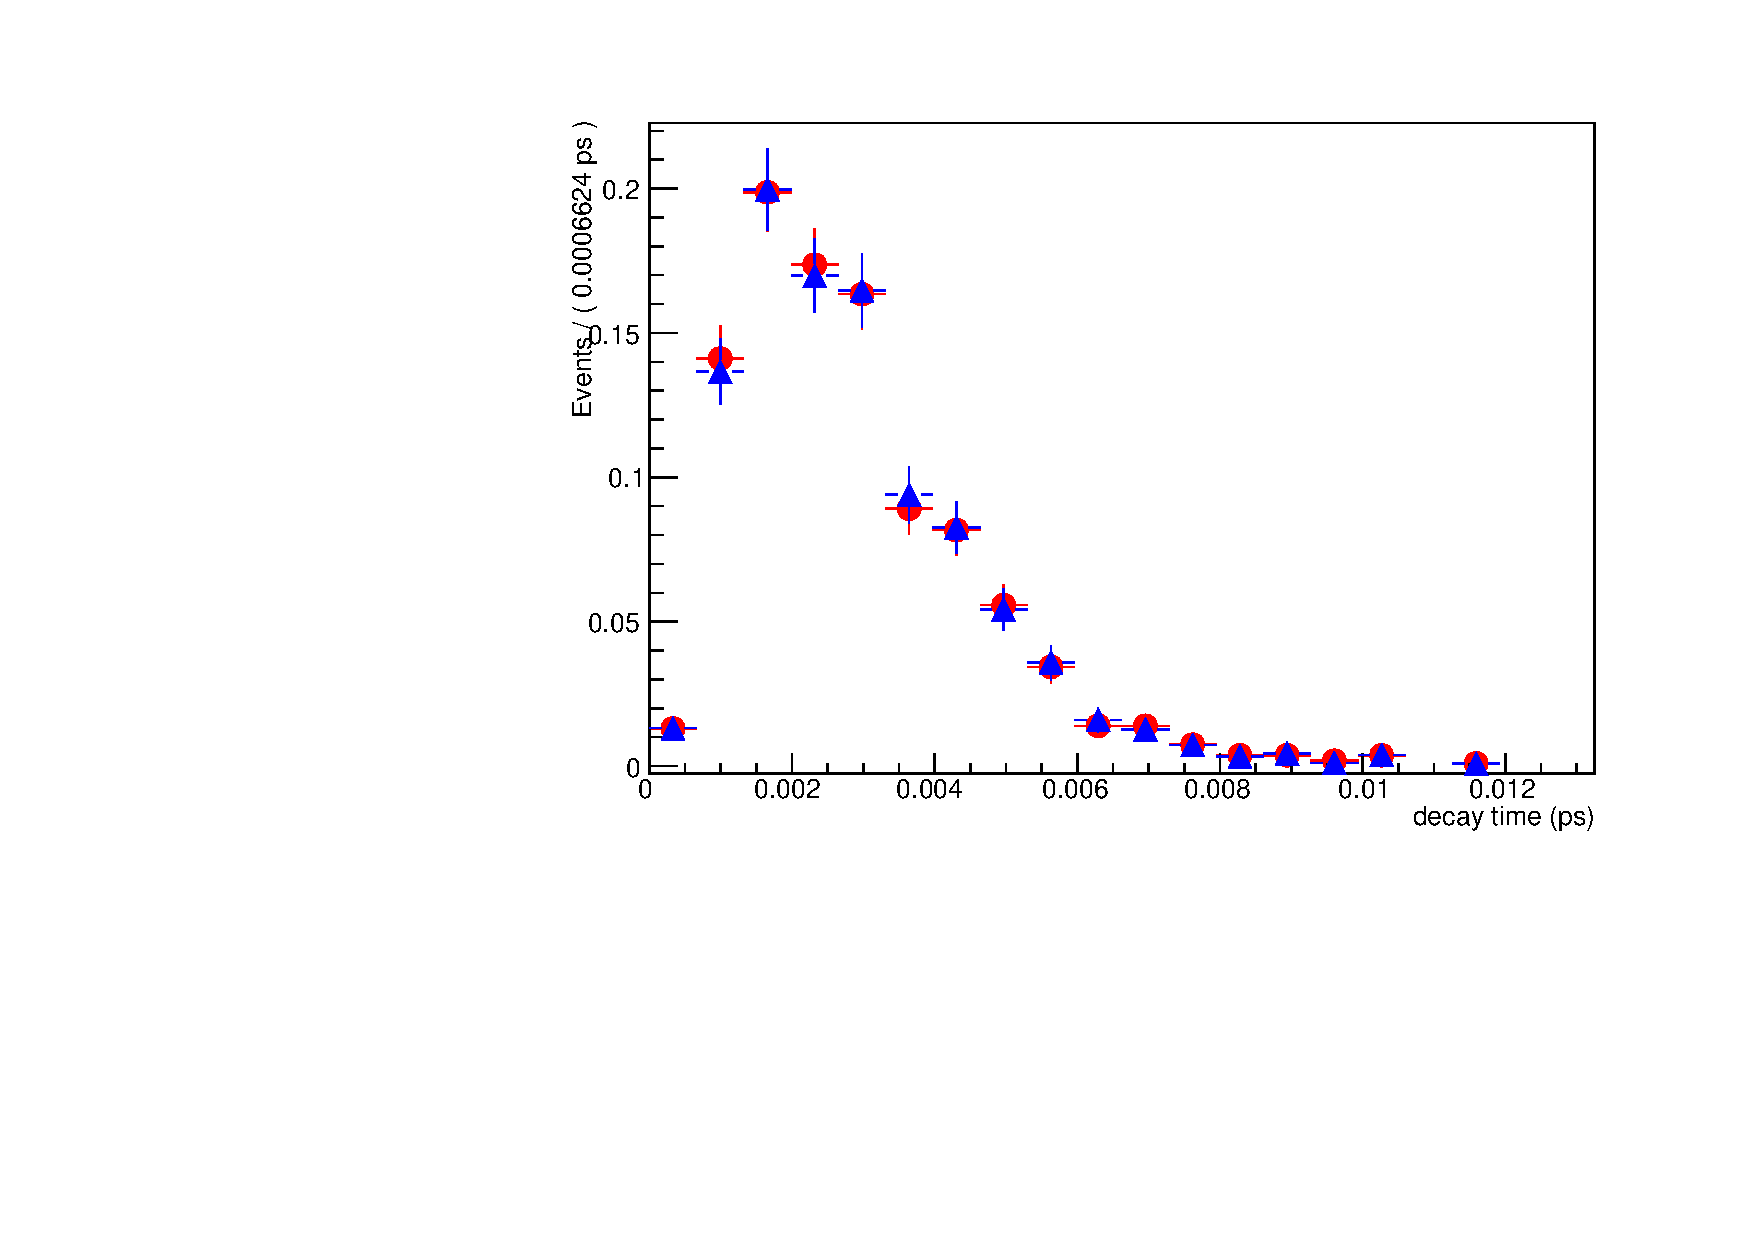
\includegraphics[width=0.49\textwidth]{./Figs/LifetimeMeasurement/2011_B_TAU_Bd2KPi_MC_weighted_and_unweighted.pdf}
    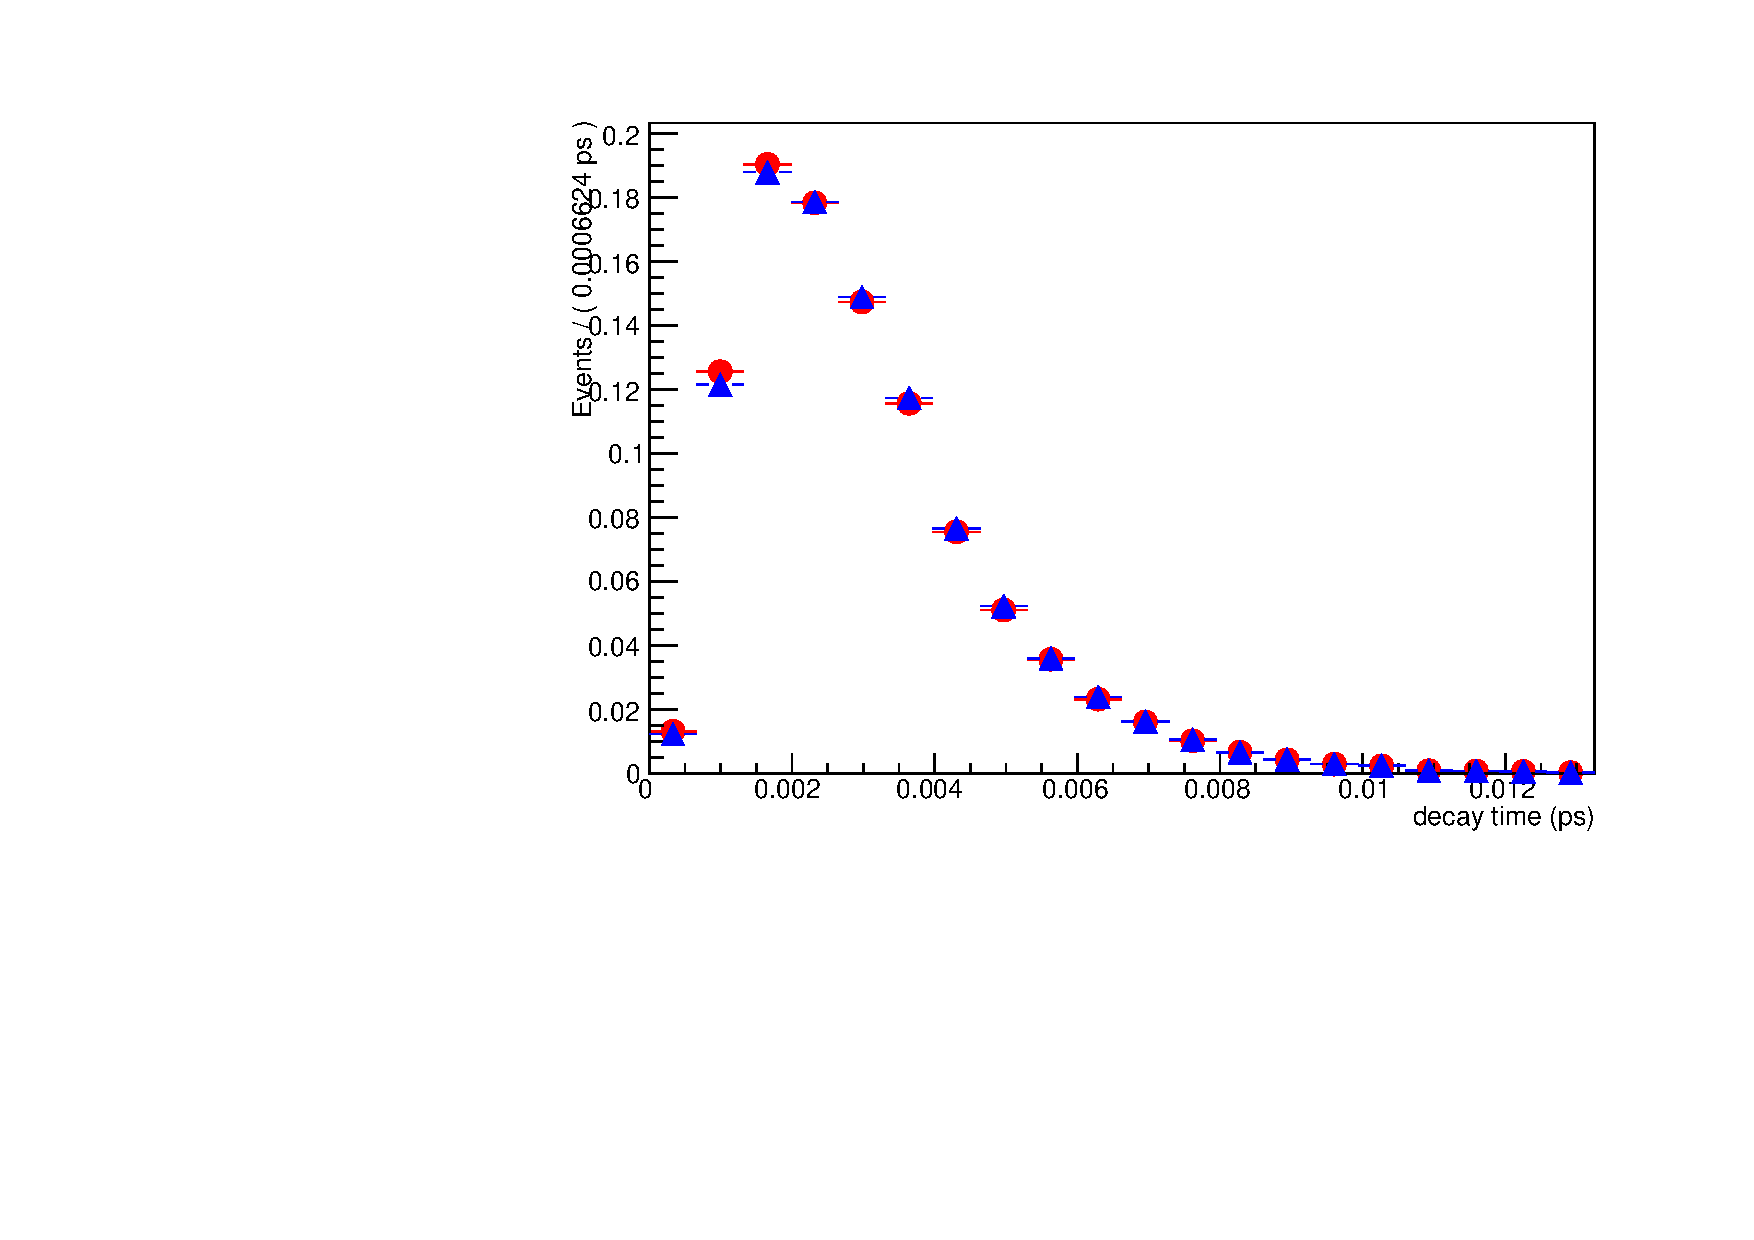
\includegraphics[width=0.49\textwidth]{./Figs/LifetimeMeasurement/2012_B_TAU_Bd2KPi_MC_weighted_and_unweighted.pdf}
    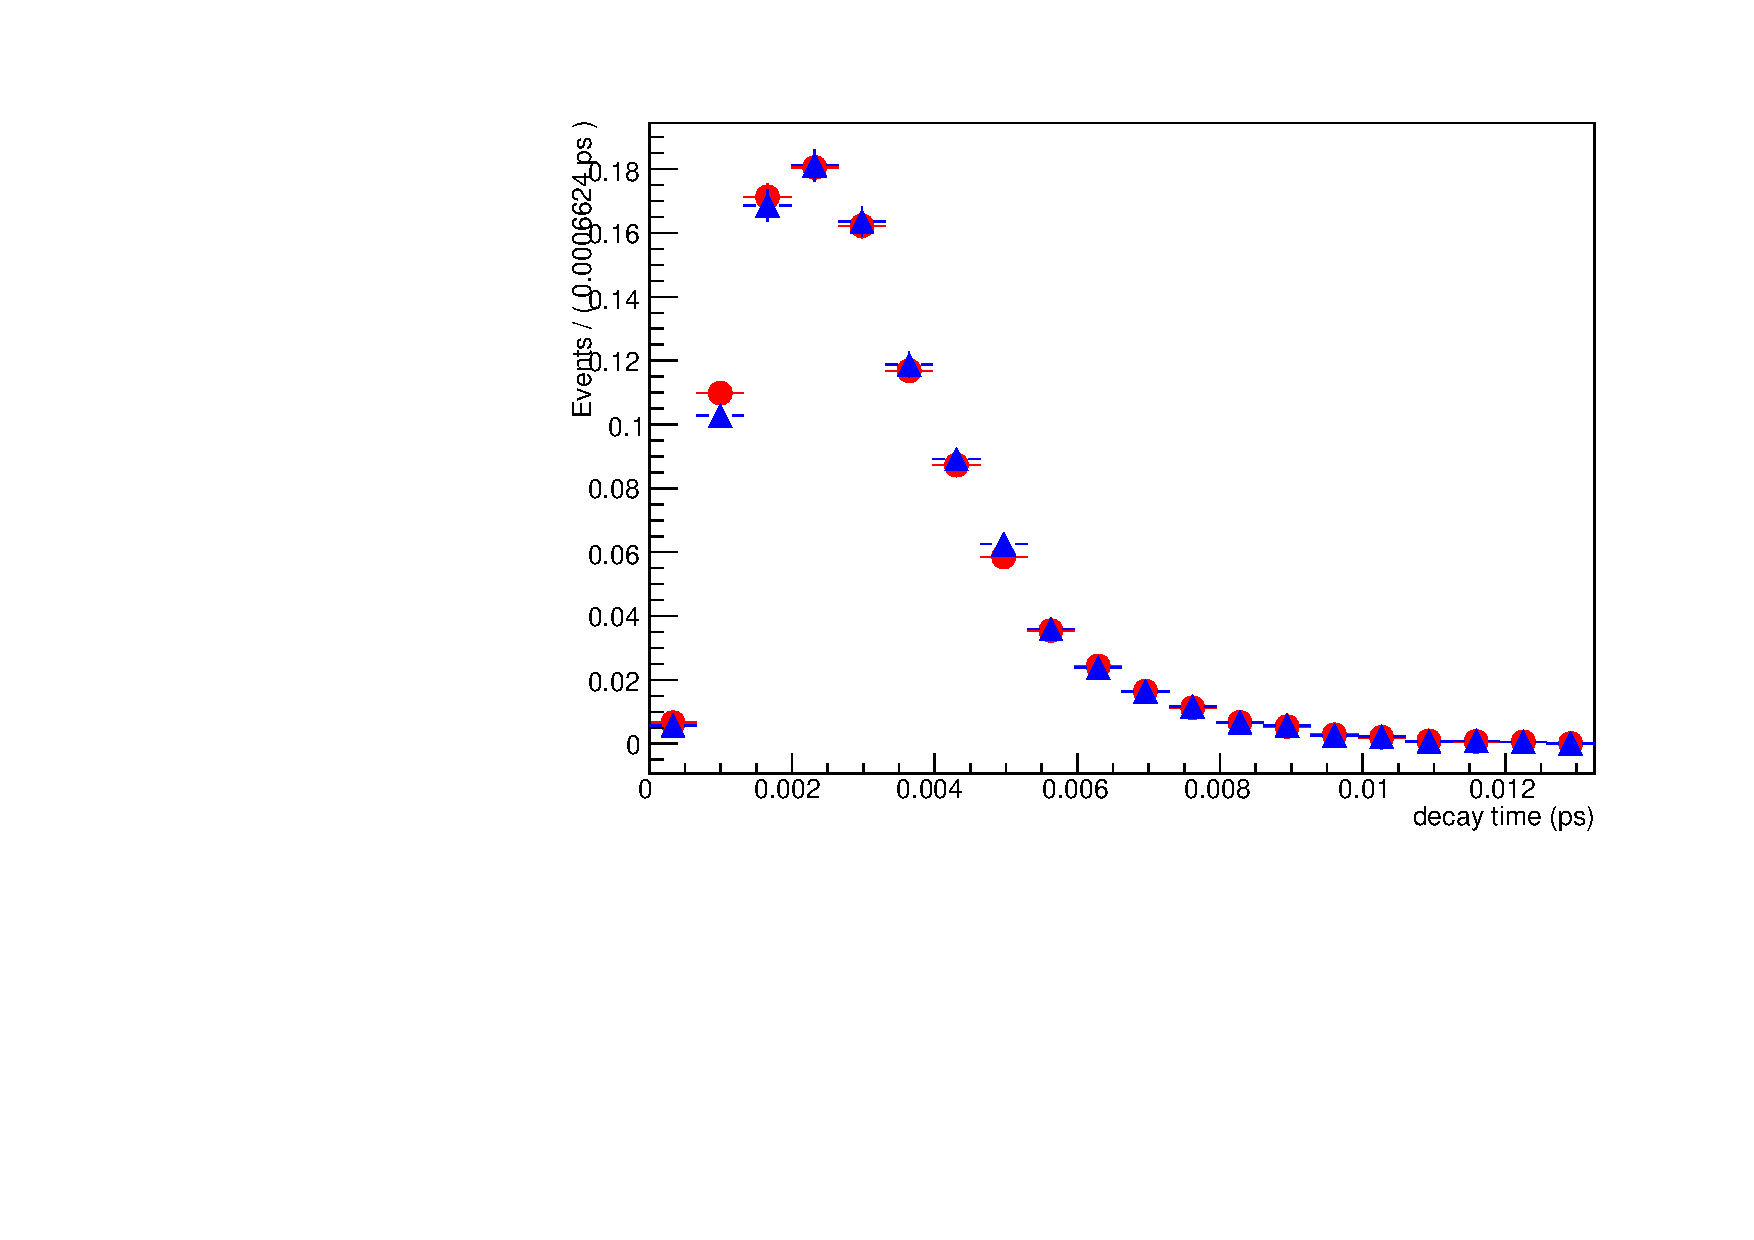
\includegraphics[width=0.49\textwidth]{./Figs/LifetimeMeasurement/2015_B_TAU_Bd2KPi_MC_weighted_and_unweighted.pdf}
    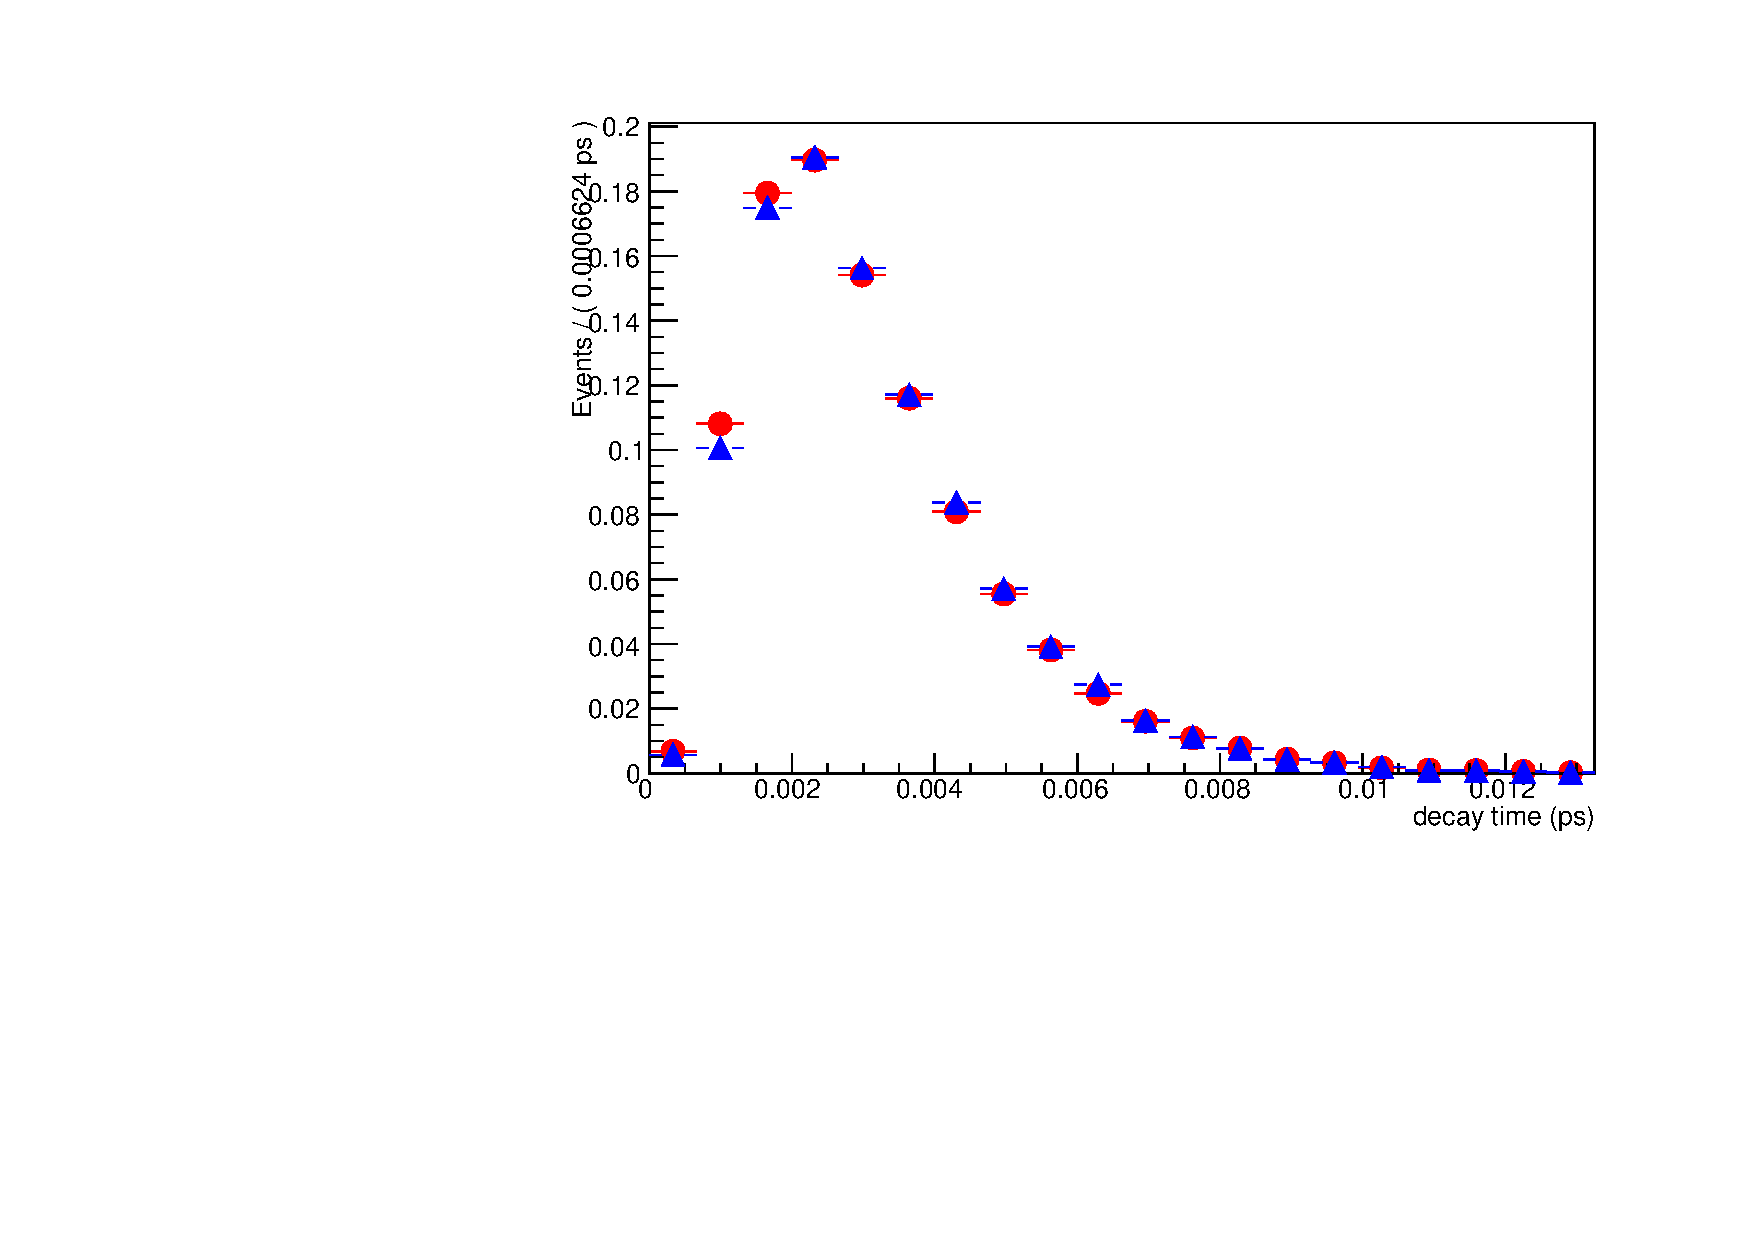
\includegraphics[width=0.49\textwidth]{./Figs/LifetimeMeasurement/2016_B_TAU_Bd2KPi_MC_weighted_and_unweighted.pdf}
  \caption{The decay time distributions for \bdkpi simulated candidates for 2011 (top left), 2012 (top right), 2015 (bottom left) and 2016 (bottom right), before (red circles) and after (blue squares) re weighting by the number of tracks, after the BDT cut and TIS trigger requirements have been applied.}
  \label{fig:BdToKpi_weightDecayTime}
\end{figure}


The same weights are applied to simulated \bsmumu decays by binning the number of tracks per event for \bsmumu decays in the same way to used for \bdkpi decays. The weights are applied to decays that pass selection but before the global BDT cut is applied. The change in the decay time distribution for \bsmuu simulated decays after the global BDT cut is shown in Figure~\ref{fig:BsmmVsBdToKpinTracks} in the comparison of weighted and un-weighted \bsmumu decay time distributions. Similarly to \bdkpi decays the biggest effect is at low decay times where the change in selection efficiency is greatest as seen in Figure~\ref{fig:accpteg}.
\begin{figure}[htbp]
  \centering
    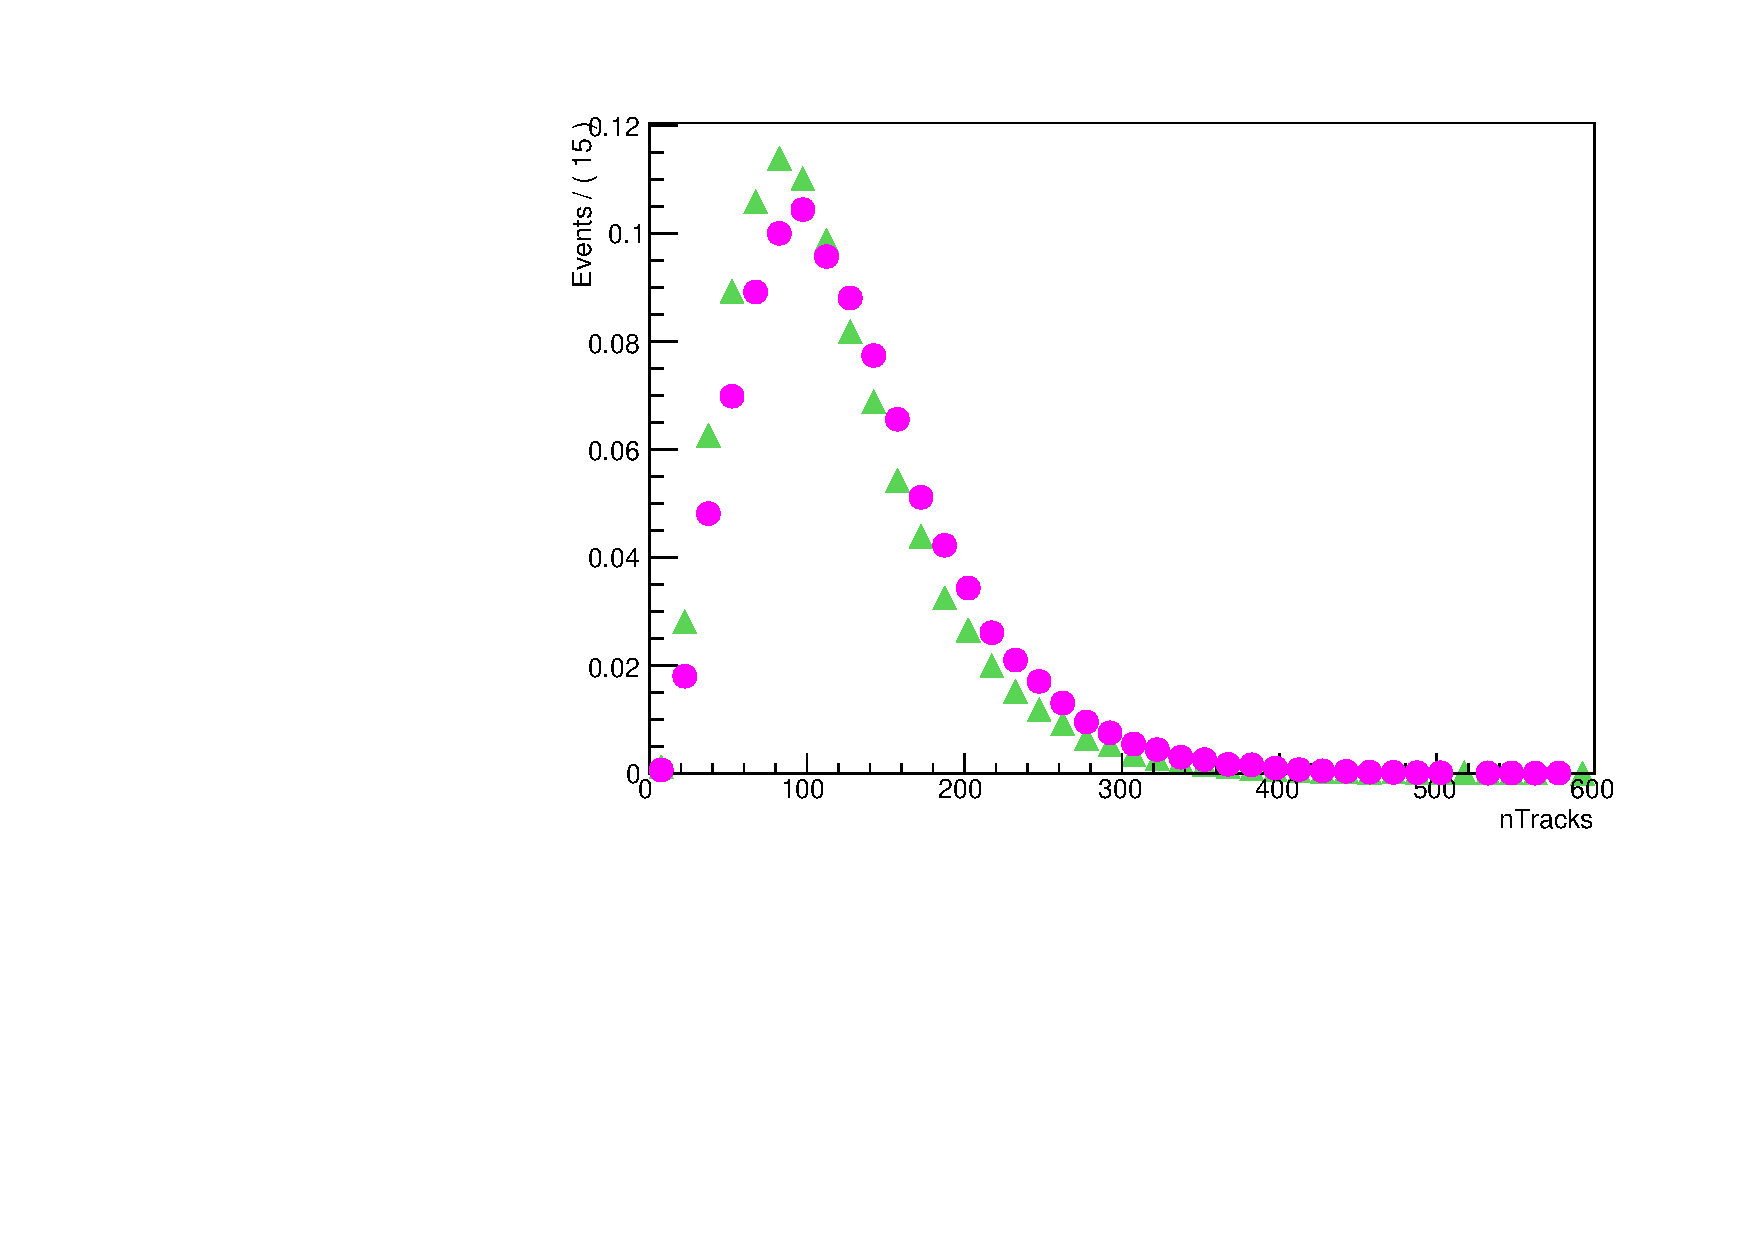
\includegraphics[width=0.49\textwidth]{./Figs/LifetimeMeasurement/nTracks_2011_Bd2KPi_Bs2MuMu_Dec_triggers.pdf}
    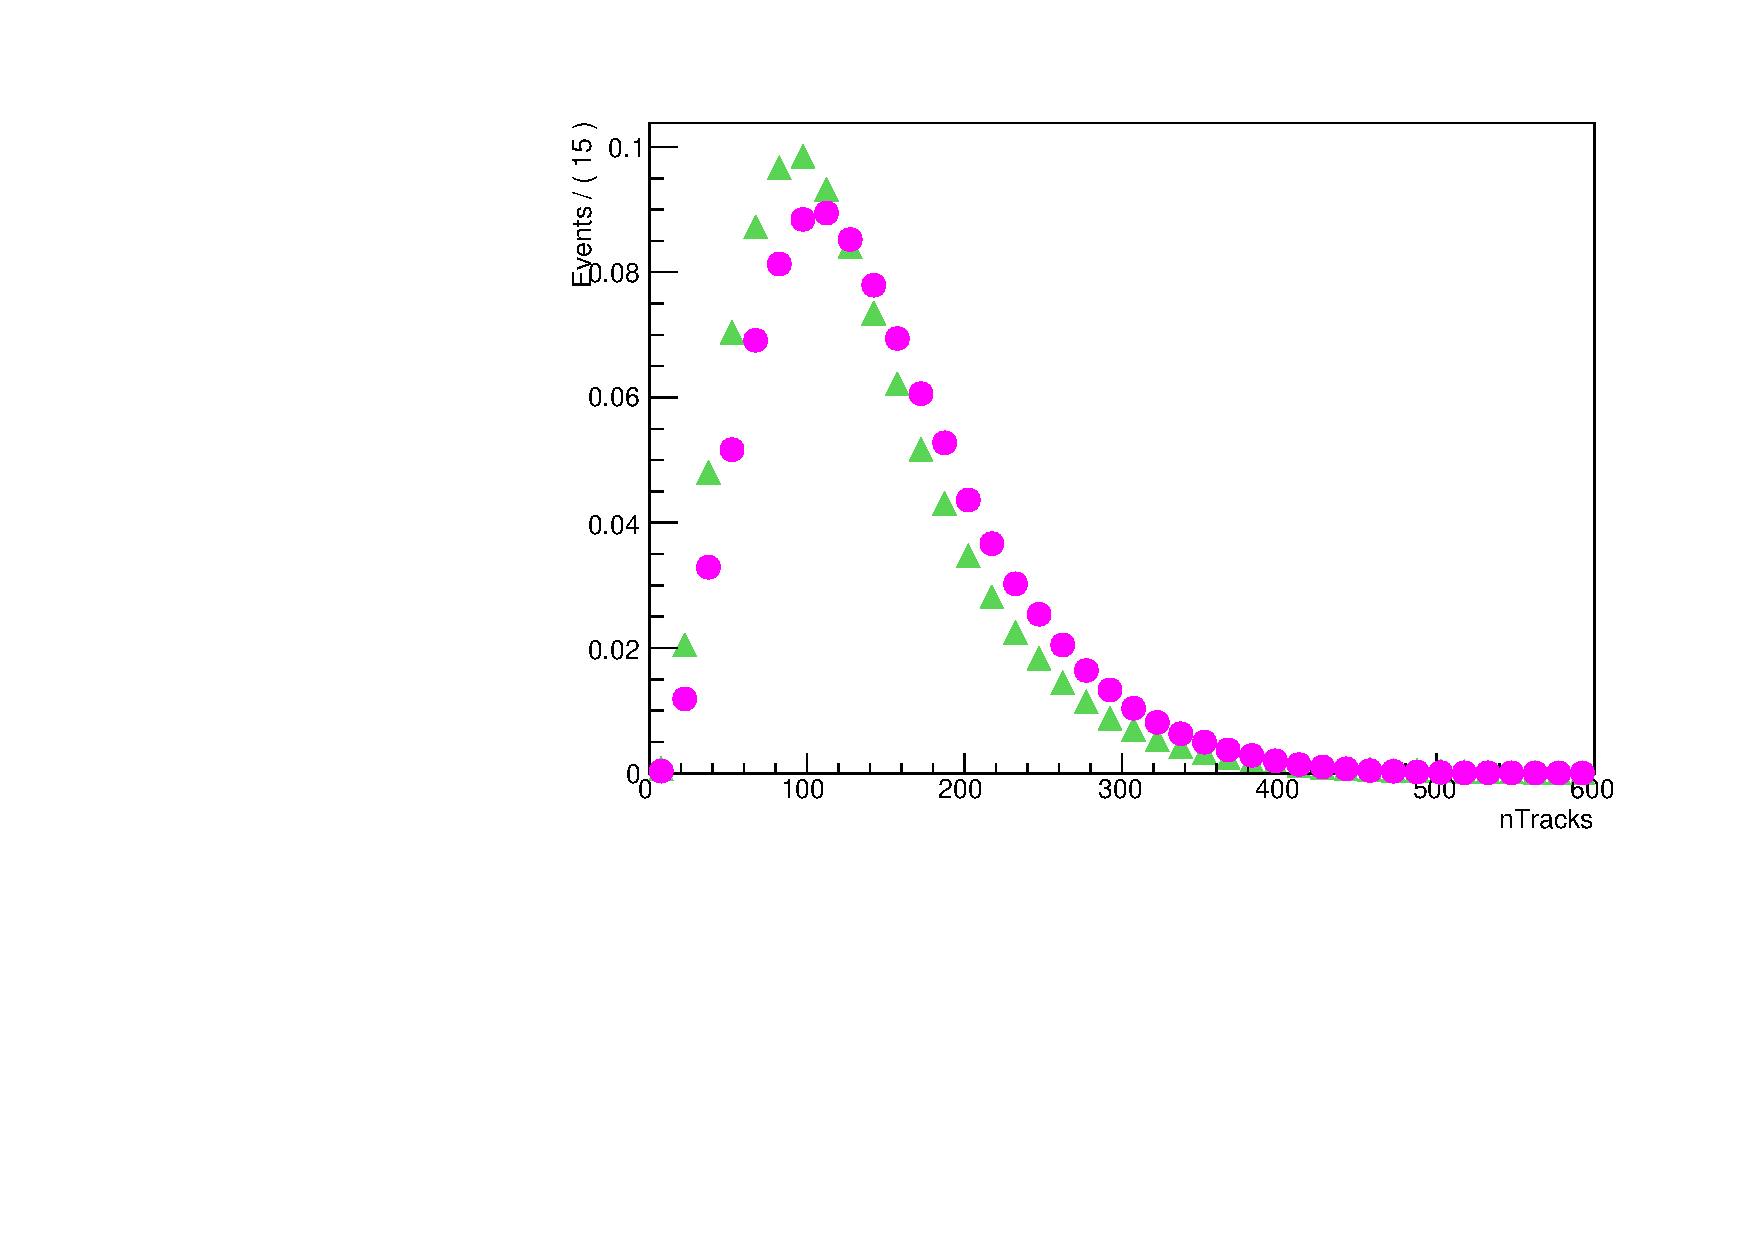
\includegraphics[width=0.49\textwidth]{./Figs/LifetimeMeasurement/nTracks_2012_Bd2KPi_Bs2MuMu_Dec_triggers.pdf}
    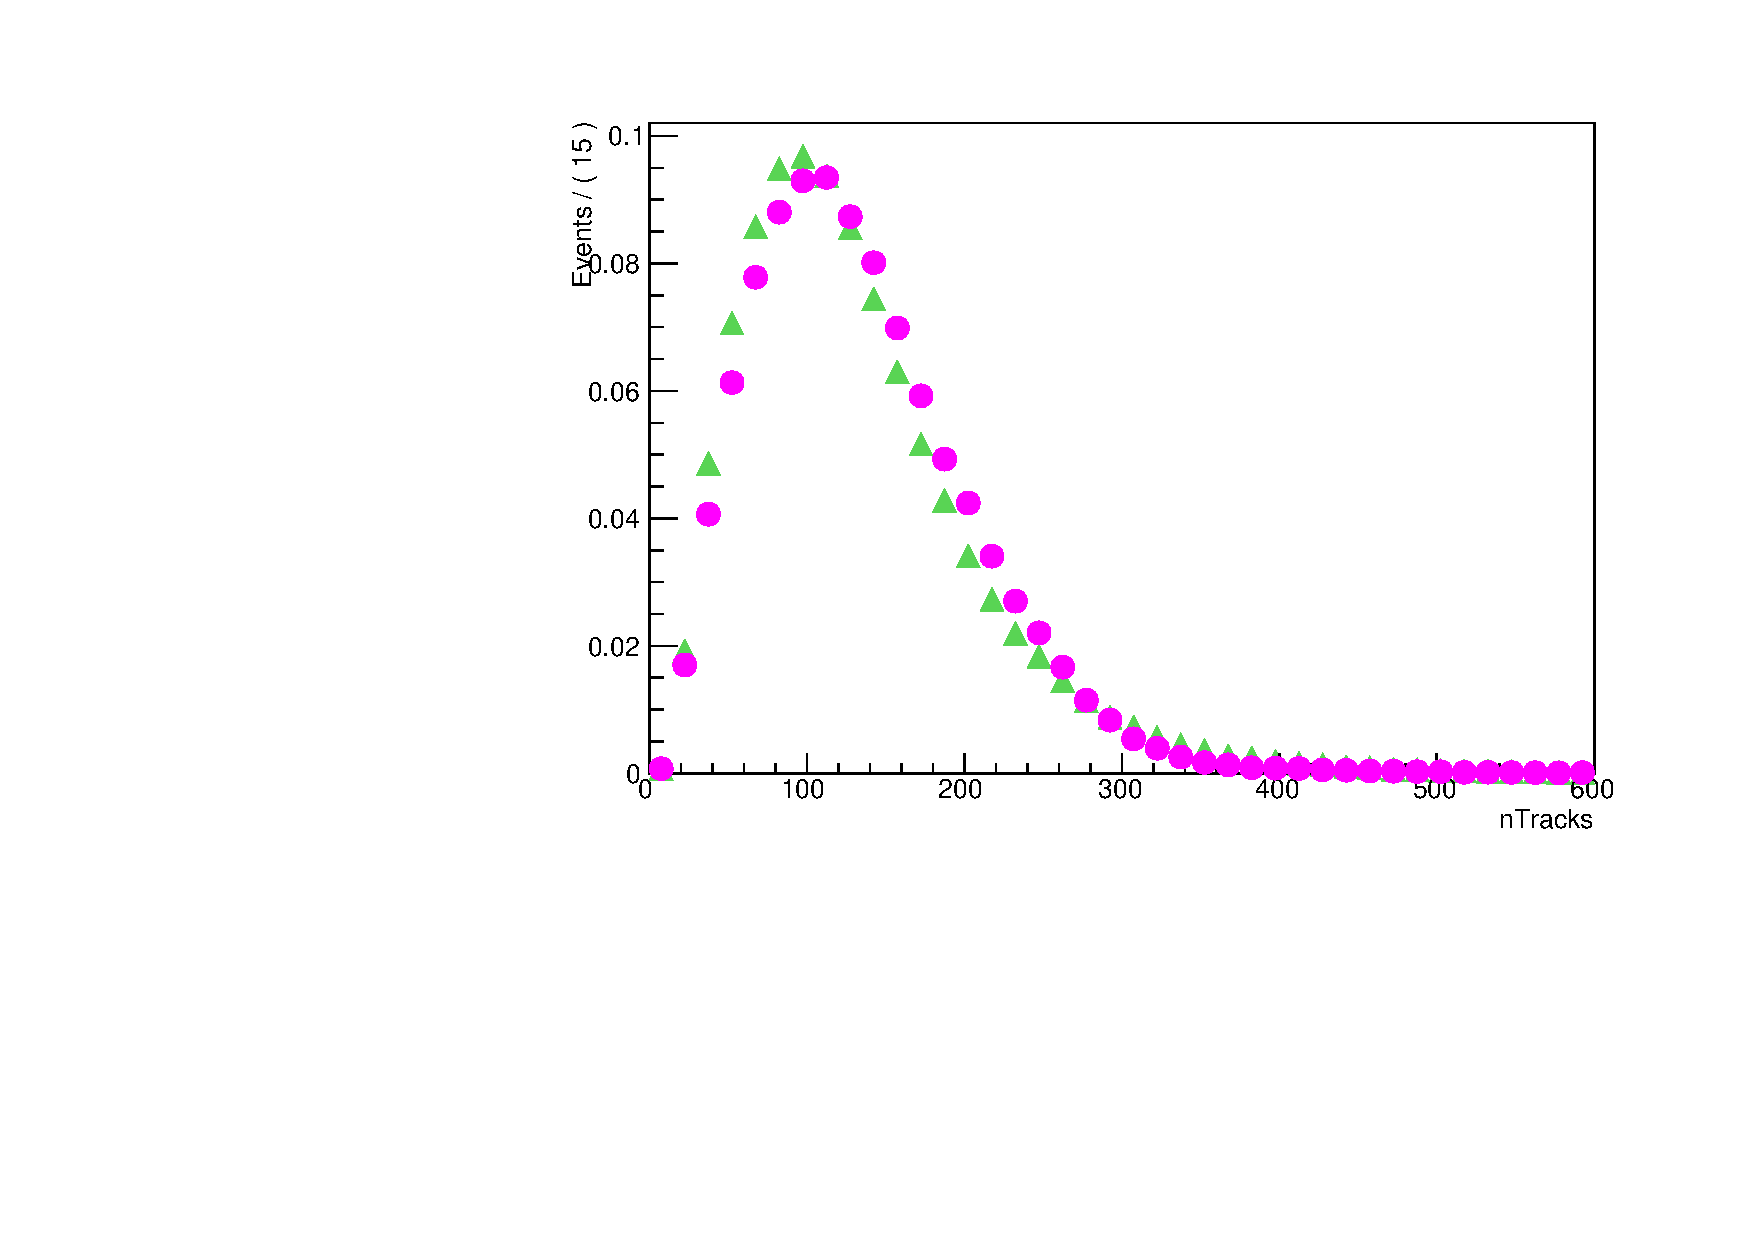
\includegraphics[width=0.49\textwidth]{./Figs/LifetimeMeasurement/nTracks_2015_Bd2KPi_Bs2MuMu_Dec_triggers.pdf}
    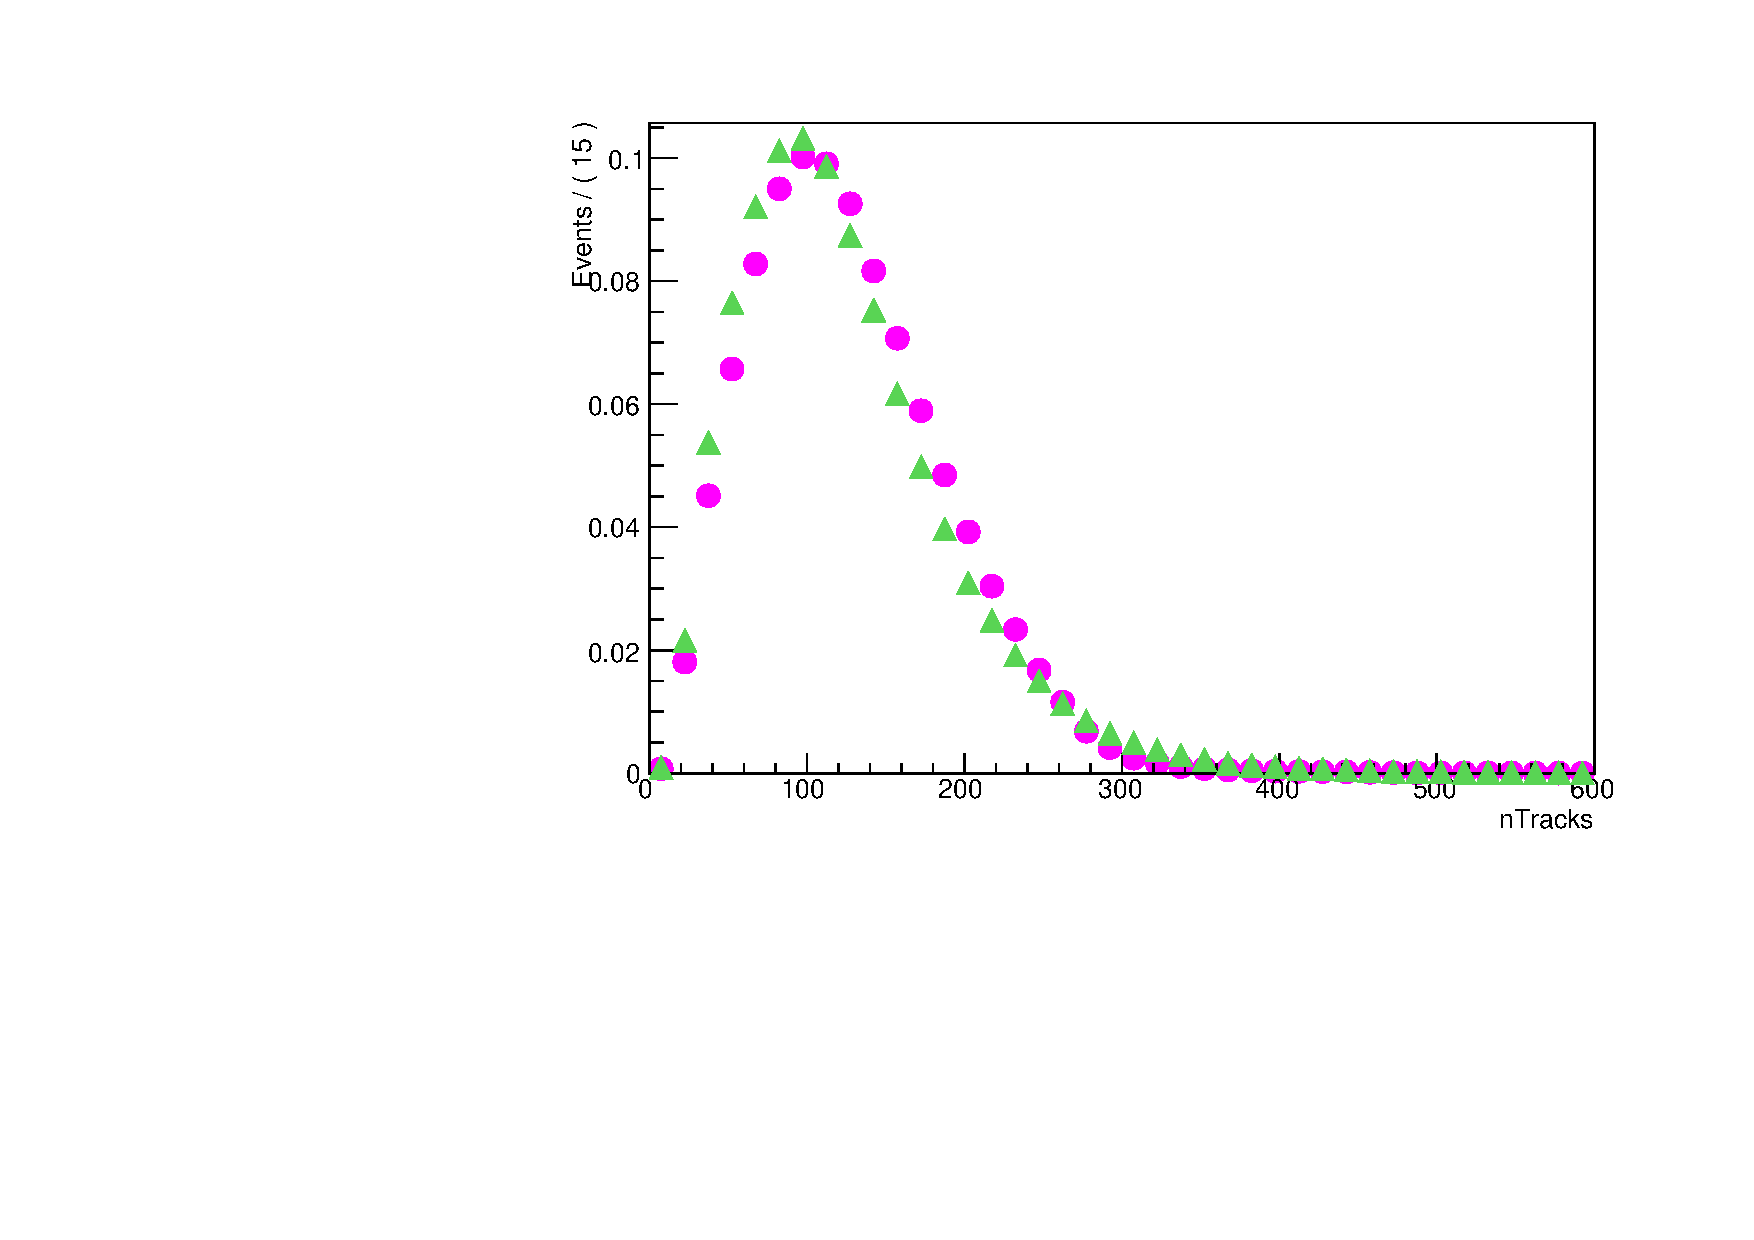
\includegraphics[width=0.49\textwidth]{./Figs/LifetimeMeasurement/nTracks_2016_Bd2KPi_Bs2MuMu_Dec_triggers.pdf}
  \caption{The number of tracks for \bdkpi (green triangles) and \bsmumu (pink circles) decays in Monte Carlo simulated events after the trigger, stripping and Prue-selection but before any BDT cut, for each year: 2011 (top left), 2012 (top right), 2015 (bottom left) and 2016 (bottom right). }
  \label{fig:BsmmVsBdToKpinTracks}
\end{figure}

The reweighing relies on the number of tracks per event being very similar for \bdkpi and \bsmumu decays, this cannot be evaluated in data due to the small number of \bsmumu decays in data. However Figure~\ref{fig:BsTomumu_weightDecayTime} shows a comparison of the number of tracks per event for simulated \bsmumu and \bdkpi decays for each year and resulting distributions are rather similar.
\begin{figure}[htbp]
  \centering
    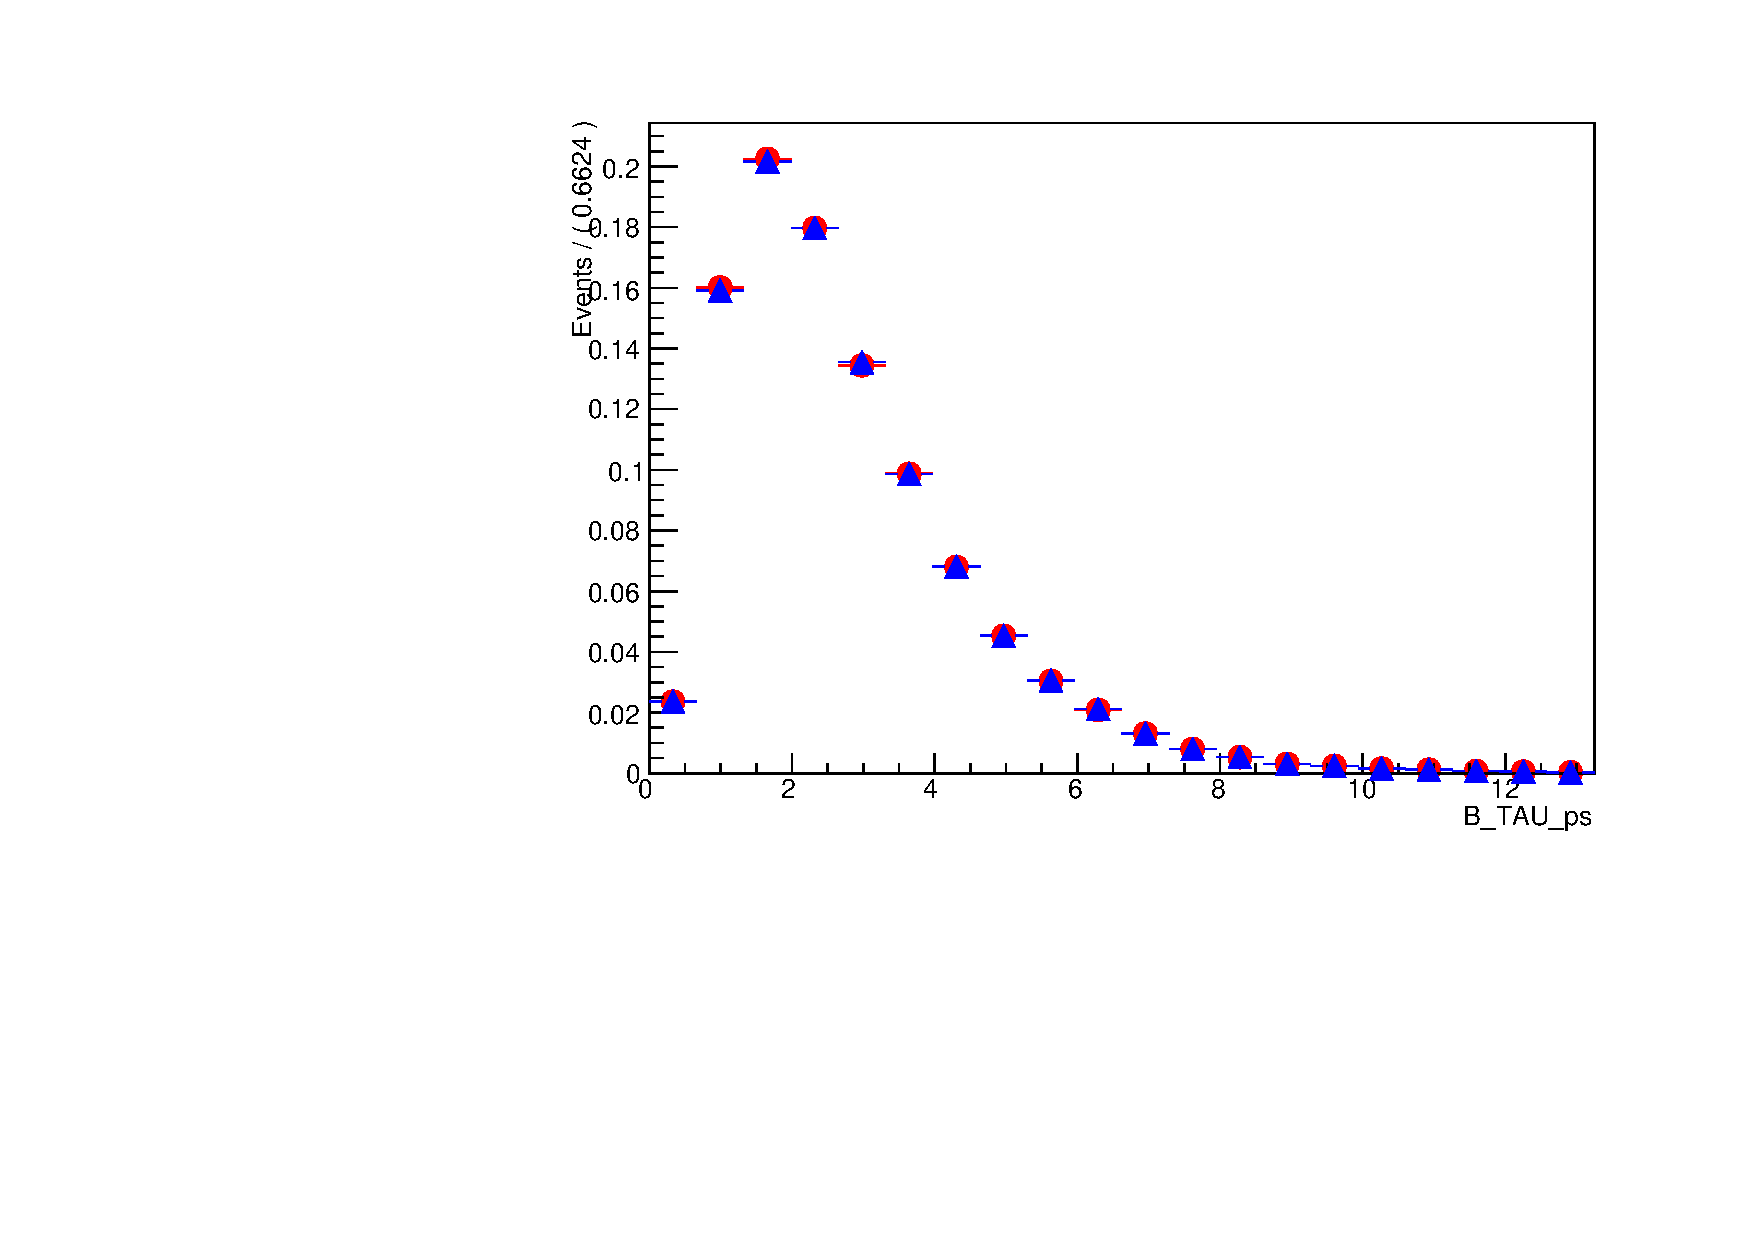
\includegraphics[width=0.49\textwidth]{./Figs/LifetimeMeasurement/2011_Bs2MuMu_MC_weighted_unweighted_comparison.pdf}
    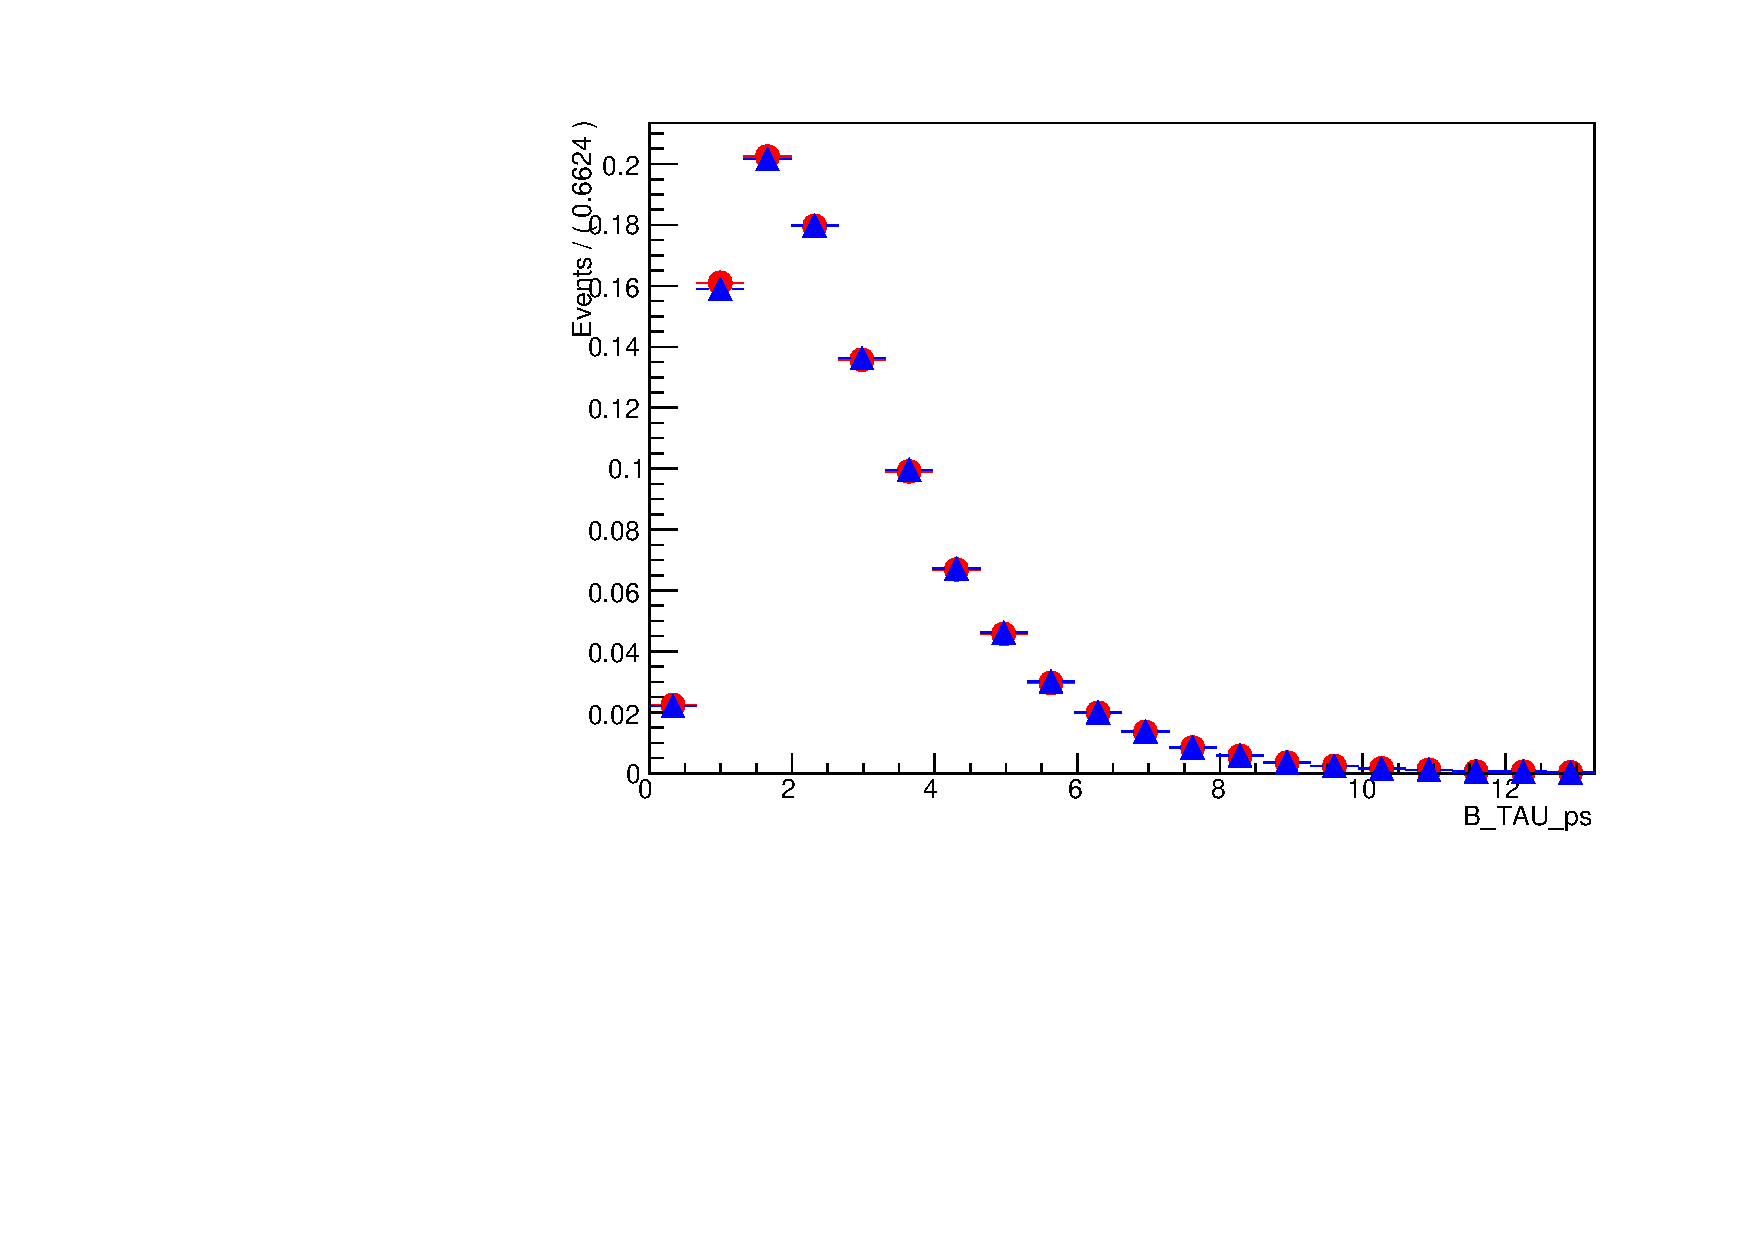
\includegraphics[width=0.49\textwidth]{./Figs/LifetimeMeasurement/2012_Bs2MuMu_MC_weighted_unweighted_comparison.pdf}
    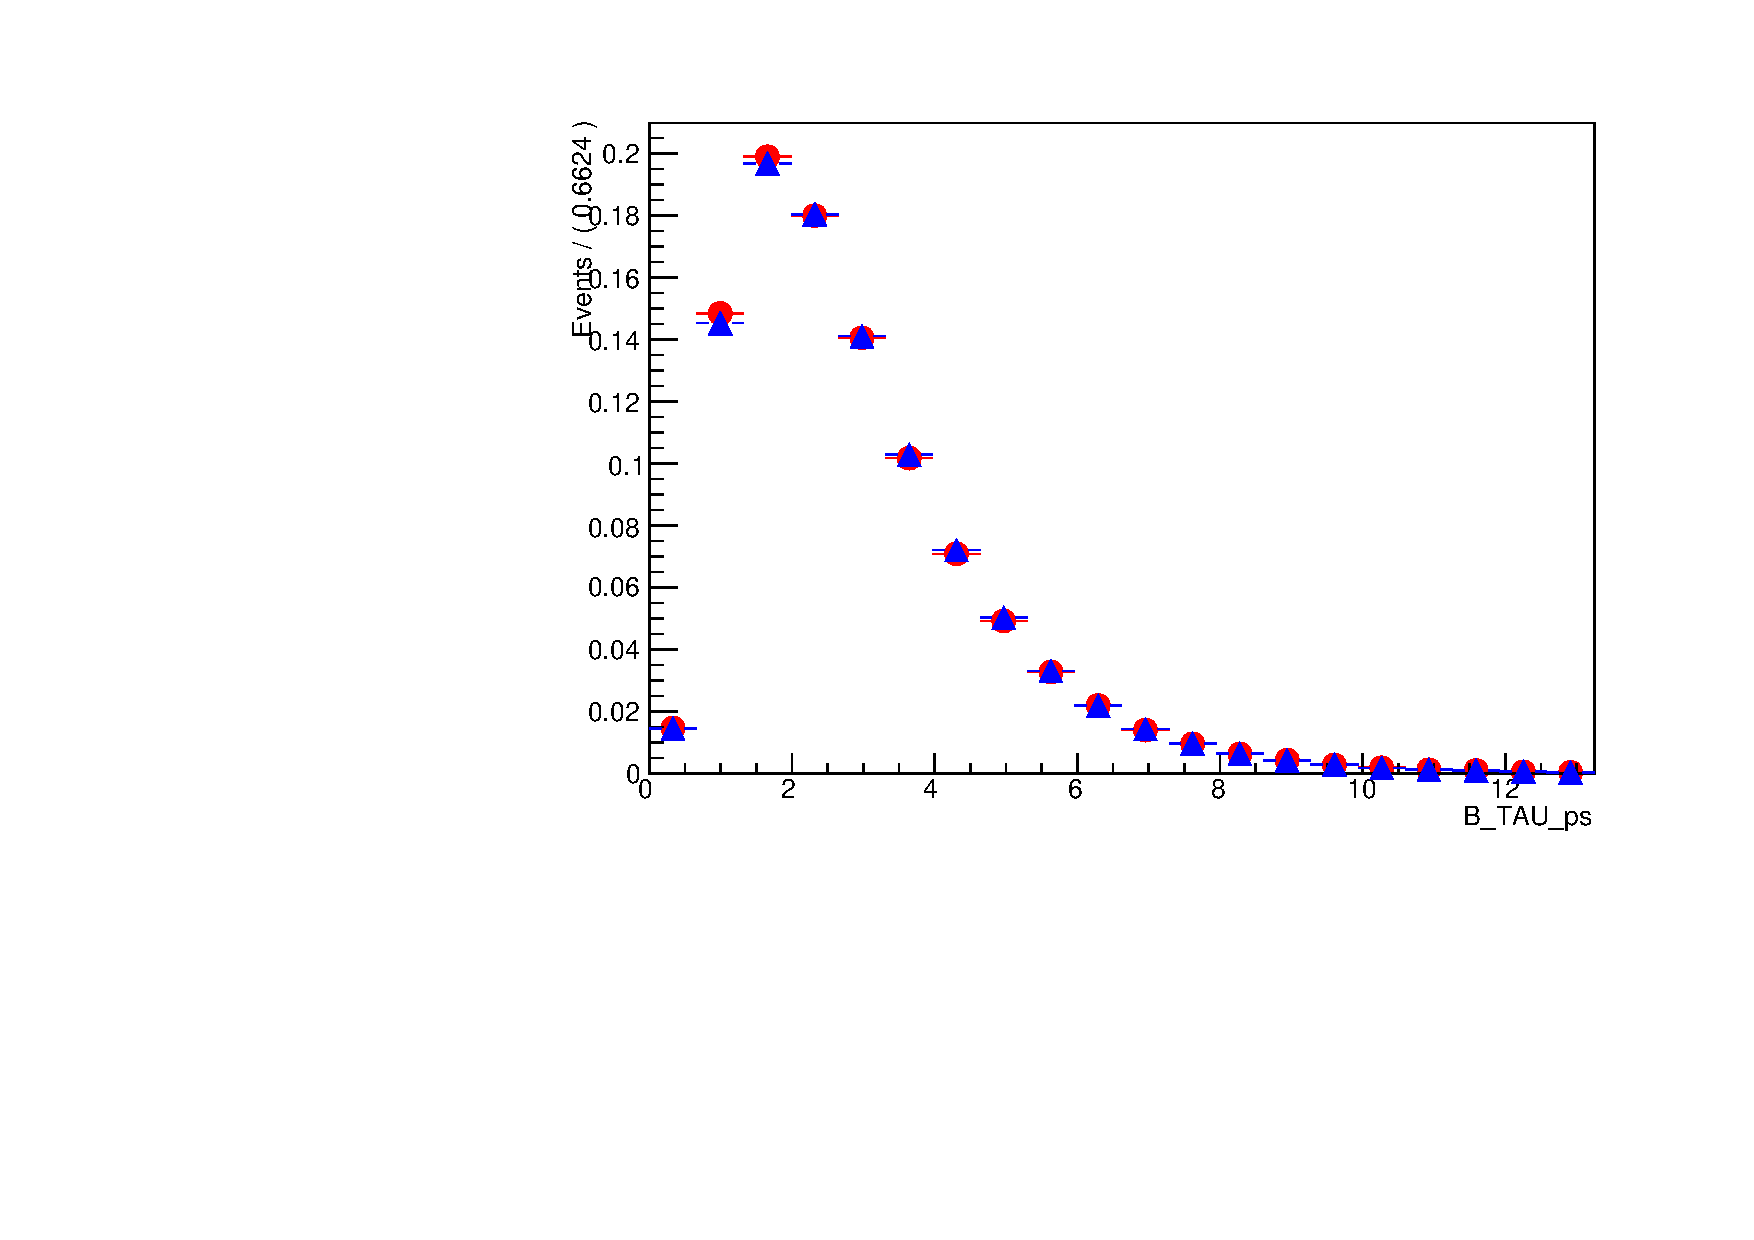
\includegraphics[width=0.49\textwidth]{./Figs/LifetimeMeasurement/2015_Bs2MuMu_MC_weighted_unweighted_comparison.pdf}
    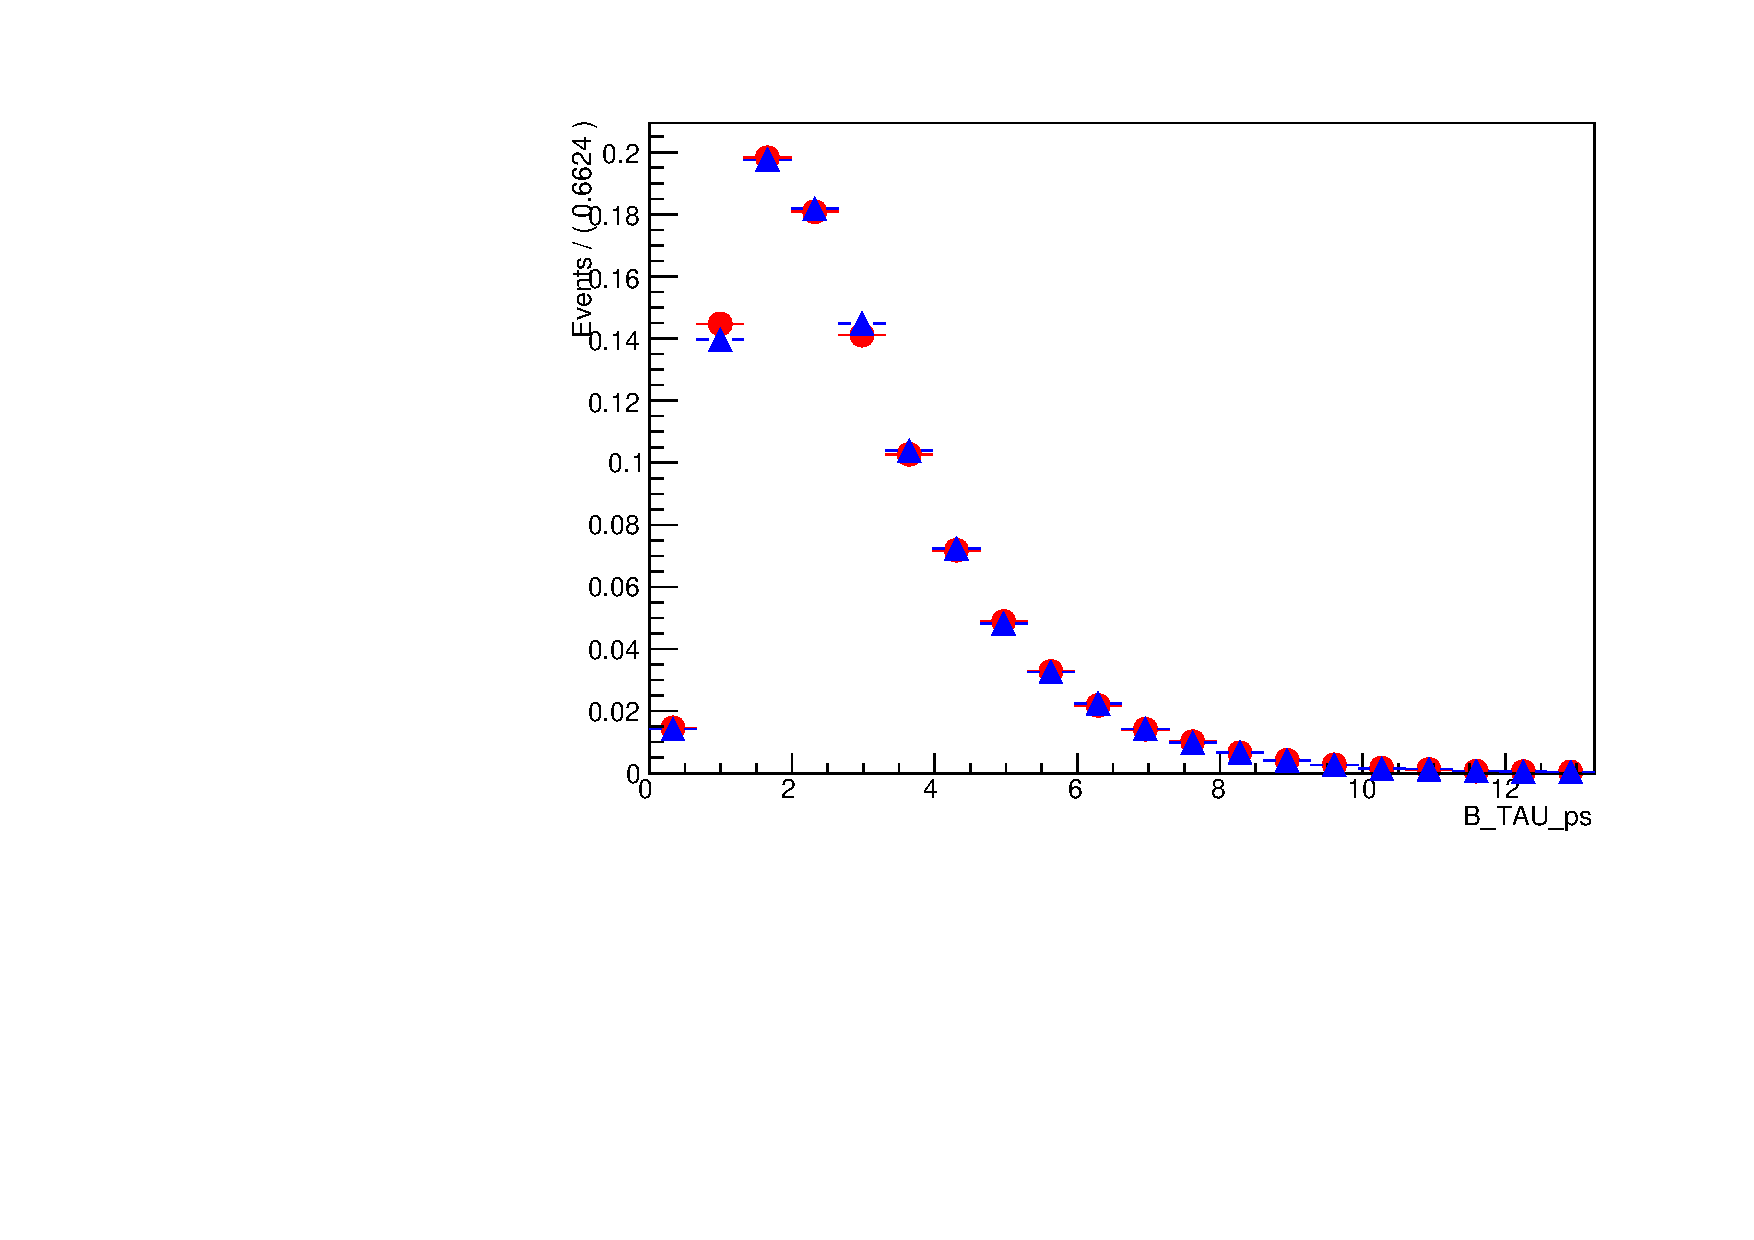
\includegraphics[width=0.49\textwidth]{./Figs/LifetimeMeasurement/2016_Bs2MuMu_MC_weighted_unweighted_comparison.pdf}
  \caption{The decay time distributions for \bsmumu simulated candidates for 2011 (top left), 2012 (top right), 2015 (bottom left) and 2016 (bottom right), before (red circles) and after (blue squares) re weighting by the number of tracks, after the BDT cut and trigger requirements have been applied.}
  \label{fig:BsTomumu_weightDecayTime}
\end{figure}

%accptance from MC problems can in Bd2kPi decays - was is just Run 2 or both? Could the problem actually have been sim09a not MC in general?

Now the decay time efficiency will be accurately modelled in the weighted simulated \bsmumu decays, the parameters in the acceptance function can be evaluated. The decay time efficiency for each year of data taking is slightly different, as illustrated in Figure~\ref{}, therefore simulated decays from each year of data taking must be used to determine the acceptance parameters. The number of simulated decays available for each year does not correspond to the proportions of decays present in each year of the data. Therefore weights are used to combine the simulated decays so that the combined set of decays has the same proportions of decays for each year as the complete data set. The weights are
\begin{equation}
\omega_{i}  = \frac{Y_{i}^{J/\psi \phi} \epsilon_{i}}{\displaystyle\sum_{j} Y_{j}^{J/\psi \phi} \epsilon_{j}} \cdot \frac{\displaystyle\sum_{k} N_{k}^{\mu^{+}\mu^{-}}}{N_{i}^{\mu^{+}\mu^{-}}}
\end{equation}
where $i$ represents the year, $N^{\mu^{+}\mu^{-}$ the number of simulated \bsmumu decays available for the year passing the full \bsmumu selection, $Y^{J/\psi \phi}$ are the yields of \bsjpsiphi decays in data that have passed the stripping, trigger and pre-selection and $\epsilon$ are the efficiencies of the BDT and particle identification cuts applied to select \bsmumu decays that have already passed the other selection requirements. {\it How much detail do I really need to put in??} The same selection is applied to \bsjpisphi decays as \bsmumu. \bsjpisphi decays are used because the production, reconstruction and selection efficiencies behave the same as \bsmumu across the different years of data taking, so the number of \bsjpisphi decays is proportional to the number of \bsmumu decays. 

The weights applied to simulated \bsmumu decays and values of the different components of the weights are given in Table~\ref{tab:MCWeightInfo}.

\begin{table}[ht]
\begin{center}
\begin{tabular}{lccccc}
\hline
Year ($i$) & $Y_i^{\JPsiPhi}$ & $\epsilon_i$ & $N^{\mumu}_i$ & $\omega_i$ & $\mathcal{N}^{\mumu}_i \equiv N^{\mumu}_i \omega_i$ \\ \hline 
2011       & 19190           & 0.412        & 70448        & 1.72       & 131364 \\
2012       & 42103           & 0.406        & 254822       & 1.03       & 262461 \\
2015       & 8571            & 0.410        & 222820       & 0.24       & 53917 \\ 
2016       & 37765           & 0.406        & 124870       & 1.88       & 235218 \\ \hline
\end{tabular}
\caption{Weights and inputs used in the weights used to re-weight simulated \bsmumu decay for each year of data taking to ensure combined cocktail of simulated decays reflects data.}
\label{tab:MCWeightInfo}
\end{center}

\end{table}
An unbinned \ml fit is performed to the combined simulated \bsmumu decay to determine the acceptance parameters in equation~\ref{}. IN the fit the acceptance parameters can float freely and the \bsmumu lifetime is constrained to the average value used to generate the simulated decays. The fit results are shown in Figure~\ref{fig:accptfit} and the acceptance parameters are given in Table~\ref{}.

{\it I don't think this is that clear but it's a start right! (I desperately hope so!)}



\begin{figure}[htbp]
    \centering
        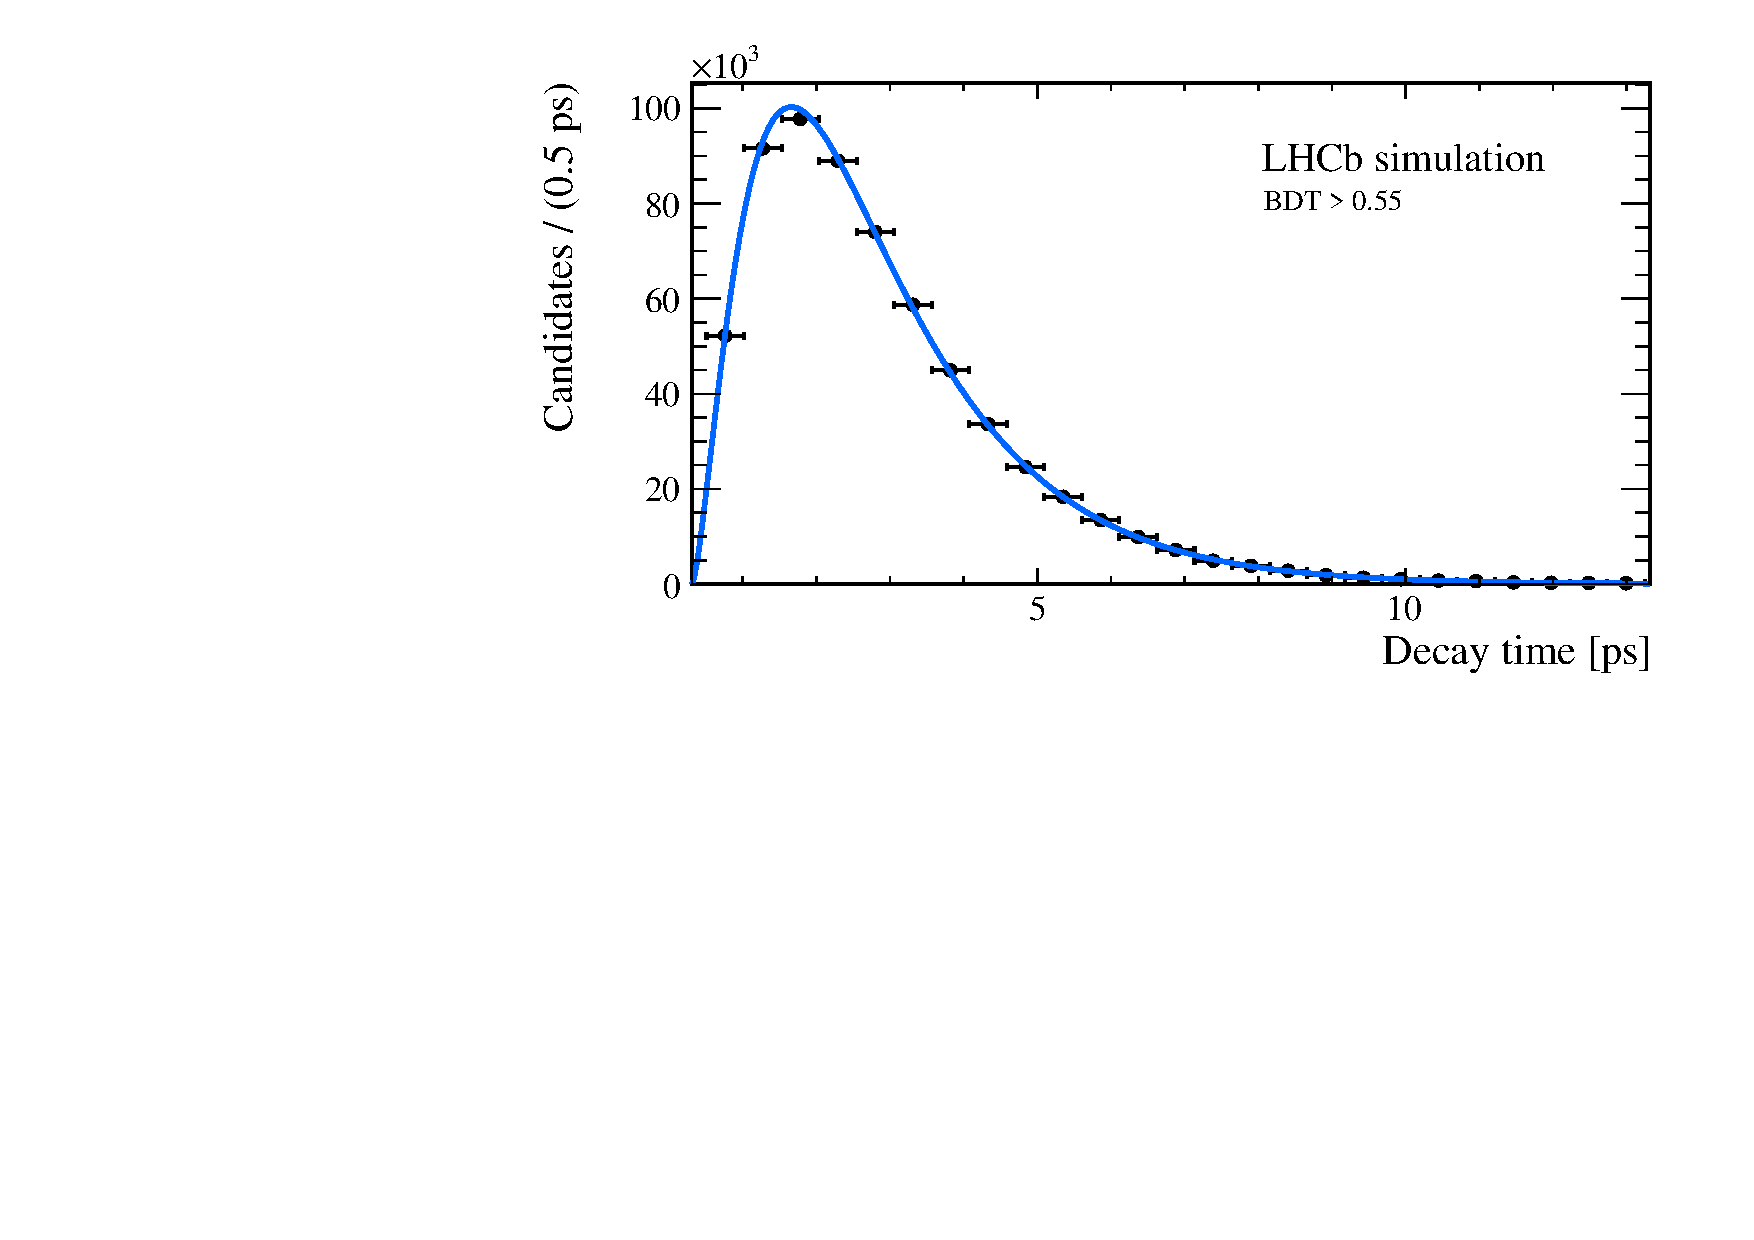
\includegraphics[width= 0.8 \textwidth]{./Figs/LifetimeMeasurement/Bs2MuMu_acceptance_fit.pdf}
    \caption{\ml fit to the combined decay time distribution for 2011, 2012, 2015 and 2016 simulated \bsmumu decays. }
    \label{fig:accptfit}
\end{figure}




\subsection{Background decay time pdf}
\label{sec:bkgDTpdf}
%Not needed in the fit but must be estimated in the toys. For exlusives we used ... for CBG we do something more complex.
{\it It needs to be clear before this point I think why these are needed and what exactly the toy studies are/aim to do.}
The final fit to measure the \bsmumu effective lifetime does not require knowledge of the decay time \pdfs of the backgrounds. However the final fit configuration is developed using toy studies that generate the mass and decay time distributions of both signal and background decays. Therefore realistic models of the decay time \pdfs are needed to determine the optimal fit configuration. 


The selection biases the decay time distributions of the backgrounds as it does the \bsmumu decay time. Therefore they are described by the same \pdfs as in equation~\ref{}. 

The backgrounds from semi-leptonic, \bhh and \bdmumu decays are assigned the same acceptance function as \bsmumu decays because the efficiency of these decays as a function of decay time is roughly similar or the same as \bsmumu decays. The acceptances of these backgrounds does not need to be as well modelled as the acceptance function of the signal because very few background decays from these sources will be present in the data set after the selection and the final results does not depend on the acceptance function of the backgrounds. The lifetimes of these decays as known, the values used in the toy studies for the decay times \pdfs are given in Table~\ref{}. {\it In the lifetime are any of the backgrounds merged?}

{\it I'm still not happy with the order of this chapter! Perhaps could split it into. 1. overview and explain that toys are needed and perhaps put the needed for the acceptance in here. 2. Signal pdf 3. Background pdf. 3. expected yields 4. Toy studies; a. outline, b. tau or 1/tau, c. actual results, d. expected sensitivity. 5. Results}

%Lets carry on for now, the order can be rearranged later! (Easier if there are acutally words to rearrange!)

The decay time \pdf of the combinatorial background is more challenging to determine. Since it arises from random combinations of muons in the event and not from one source, there is no lifetime that describes the background. Furthermore the global BDT which is designed to separate \bsmumu decays from combinatorial background decays will have a will have a different efficiency as a function of decay time for the combinatorial background compared to the \bsmum signal. The decay time \pdf of the combinatorial background cannot be evaluated from simulated decays or decays in data that pass the full \bsmumu selection, including the global BDT cut, because there are too few candidates left. The decay time \pdf must be evaluated after the global BDT cut because it has the greatest impact on the shape of the acceptance function. Therefore the decay time \pdf of the combinatorial background passing the \bsmumu selection is evaluated in candidates in data that pass the \bhh selection and have a reconstructed mass greater than 5447 \mevcc, above the \bs signal region. The decay time \pdf for combinatorial background decays is modelled by
\begin{equation}
PDF_{cbg}(t) = \epsilon(t)\times \left( f \cdot e^{-\Gamma_{2}t} + (1-f)\cdot e^{-\Gamma_{2}t} \right)
\label{eq:cbgDTpdf}
\end{equation}
where $\Gamma_{1}$ and $\Gamma_{2}$ are two independent lifetimes used to describe the background, $f$ describes the fraction of candidates with each lifetime and the same acceptance shape as in equation~\ref{} is used for describe the decay time efficiency. The lifetimes are different, one desciiibed the long lived part the other a short lives part that are evident in the data. The decay time acceptance is expected to be flat at large decay times, therefore the lifetimes of the combinatorial background decays are determined from a \ml fit of the two decaying exponential to candidates with a decay time above X. The acceptance function parameters are then determined from a \ml fit to the full decay time range using the \pdf in equation~\ref{eq:cbgDTpdf} where the lifetimes and the fraction of candidates with each lifetime are fixed. The results are shown in Figure~\ref{fig:CBGaccpt} and the \pdf parameters in Table~\ref{tab:bkgparams}, the $t_{0}$ parameter is fixed in the fit to improve stability of the fit. This model for the background assumes that the decay time distribution of \bhh candidates formed by random combinations of kaons and pions is the same as that of \bsmumu candidates formed by randomly combining muons in the event. There are too few candidates passing the \bsmumu selection to verify this assumption and the validity of this model and the impact of the toy studies is investigated in Section~\ref{}.%however the average decay time of \bhh and \bsmumu candidates with a mass above 5600 \mevcc is evaluated in bins of BDT. The results are shown in Table~\ref{}, the average decay times are not significantly different for \bhh and \bsmumu candidates therefore the decay time \pdf described here is a good model for the combinatorial background in the toy studies.
\begin{table}[ht]
\begin{center}
\begin{tabular}{lc}
\hline
Parameter & Value \\
\hline
$a$ & 1.45 $\pm$ 0.12 \ps$^{-1}$\\
$n$ & 1.92 $pm$ 0.17 \\
$t_{0}$ & 0.290 \ps \\
$\Gamma_{2}$ & $0.77 \pm 0.17$ \ps$^{-}$ \\
$\Gamma_{1}$ & $0.05 \pm 0.05$ \ps$^{-}$ \\ 
$f$ & 0.032 $\pm$ 0.027 \\
\hline
\end{tabular}
\caption{Paramerters to described the background decay time distrubution from combinatorial background decays in data passing the \bhh selection with masses between 5600 - 6000 \mevcc all data in 4.4 \fb.}
\label{tab:bkgparams}
\end{center}
\end{table}

\begin{figure}[htbp]
    \centering
   \begin{subfigure}[b]{0.48\textwidth}
        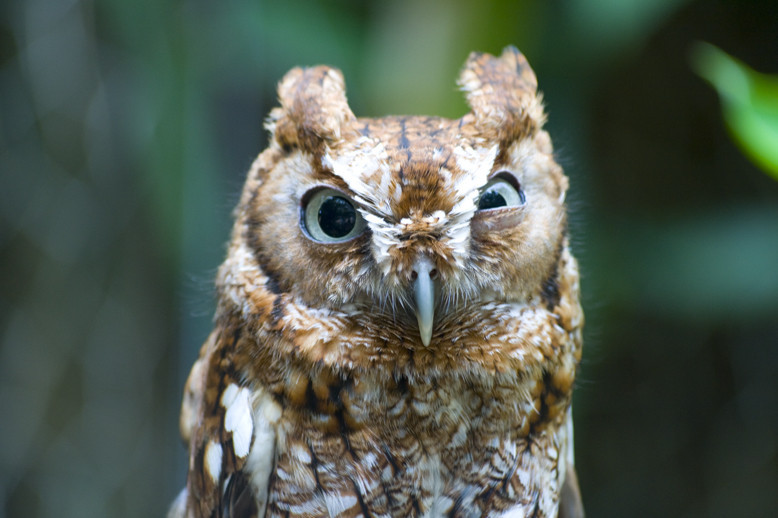
\includegraphics[width= \textwidth]{./Figs/placeholder.jpeg}
        %\caption{ }                                                                                                                    
        %\label{fig:BDTSsig}                                                                                                            
    \end{subfigure}
   ~ %add desired spacing between images, e. g. ~, \quad, \qquad, \hfill etc.                                                         
      %(or a blank line to force the subfigure onto a new line)                                                                         
    \begin{subfigure}[b]{0.48\textwidth}
       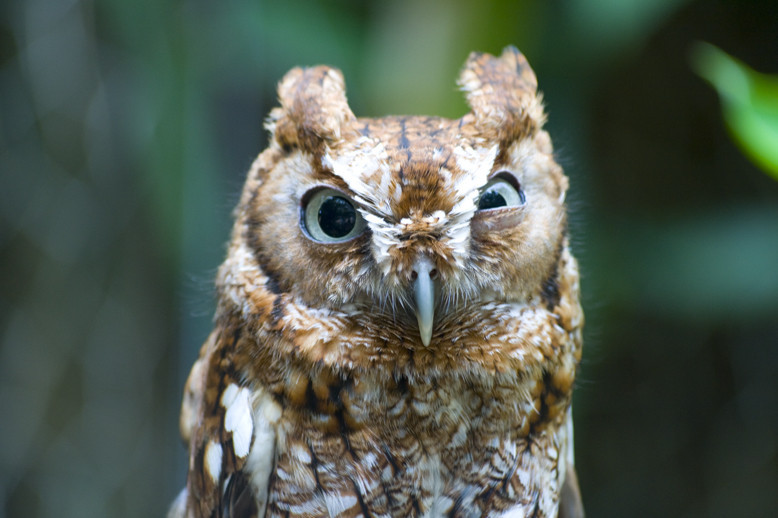
\includegraphics[width=\textwidth]{./Figs/placeholder.jpeg}
      %  \caption{ }                                                                                                                    
     %   \label{fig:BDTSbkg}                                                                                                            
   \end{subfigure}
    \caption{The \ml to determine the lifetimes of the background (left) and the acceptance parameters (right) of combinatorial background decays in data passing the \bhh selection requirements.}
    \label{fig:CBGaccpt}
\end{figure}


\section{Toy Studies for fit optimisation}
\label{sec:toys}
The strategy to measure the \bsmumu effective lifetime was described earlier in Section~\ref{}, however given the extremely rare nature of \bsmumu decays, the stability and performance of the final fit will be highly dependant on \ml fit to the invariant mass distribution. Toy studies were performed to determine which mass range, and consequently which backgrounds must be included in the \ml fit, would produce the smallest expected uncertainty on the measured effective lifetime for the data set. 

The expected number of signal and background decays in the data set passing the \bsmumu selection in the mass range 4600 - 6000 \mevcc were used as the basis for the toy studies. The expected yields were calculated using the same methods described in Chapter~\ref{} for the \bmumu branching fraction analysis but taking into account the looser particle identification requirement and the cut places on the global BDT. The number of \bsmumu and \bdmumu decays assumed the predicted branching fraction in the Standard Model. The expected yields are shown in Table~\ref{}. 

The toy studies are performed by generating the mass and decay time distributions for the expected number of signal and background decays using the \pdfs described in Section~\ref{} and~\ref{}. Then sWeights are computed from an unbinned \ml fit to the invariant mass distribution and the lifetime and its inverse are measured by a unbinned \ml fit to the signal weighted decay time distribution. A series of different mass ranges and background components in the mass fit were tested. For each possible configuration 10,000 toy studies were performed and the performance of each configuration was evaluated using using a couple of different metrics. The first is the median expected uncertainty of the \bsmumu lifetime and inverse lifetime, the median rather than the mean uncertainty is used due to the asymmetric spread of uncertainties observed for the expected statistics. The second measure is the pull distributions of any free parameters in the fit, where the pull is defined as $(x - \mu)/\sigma$ with $x$ the measured parameter value, $\mu$ the value used to generate the toys and $\sigma$ the uncertainty on the measured parameter value. Ideally the pull distributions will be Gaussian in shape with a mean at 0 and a width of 1.

 The details of the toy studies performed are given in Section~\ref{} however first is a discussion of whether the \bsmumu lifetime or inverse lifetime should be measured given the expected number of decays present in the data set.  

\subsection{To fit for $\tau$ or $\tau^{-1}$}
\label{sec:tauORinvtau}
During the development of the fit storage the toy studies produced biased pull distributions for the \bsmumu effective lifetime no matter what mass fit configuration was used and when no acceptance function was used in the decay time \pdfs. The pull distribution for \tmumu is shown in Figure~\ref{fig:taupulls} for a simplified study where no acceptance function is used and only signal and combinatorial background decays are generated, the distribution is clearly not Gaussian in shape. The bias was more pronounced in early stages of the analysis development which was done assuming the expect signal and background yields of only the Run 1 data set. 

\begin{figure}[htbp]
    \centering
        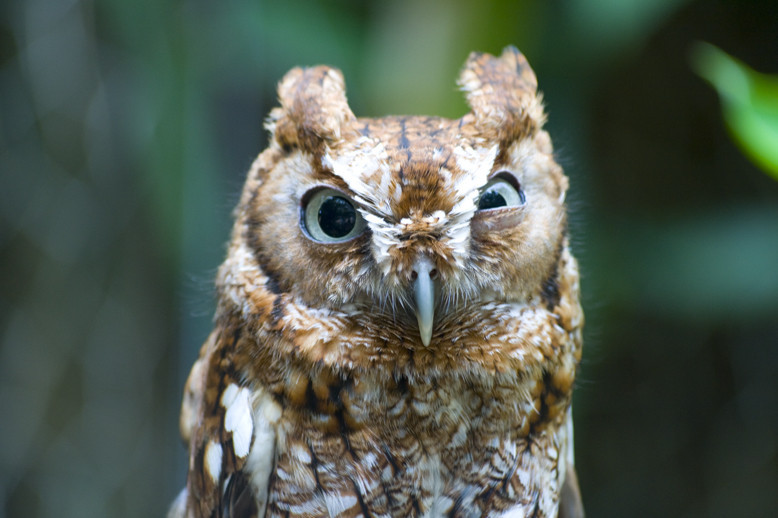
\includegraphics[width= 0.6 \textwidth]{./Figs/placeholder.jpeg}  
    \caption{Pull distribution for \tmumu using simplified toys for the expected statistics of the data set 4.4 \fb.}
    \label{fig:taupulls}
\end{figure}

The log-likelihood profile of the decay time fit at a function of \tmumu reveals the cause of the biased pull distribution. For the simplified studies illustrated in Figure~\ref{fig:taulike} the decay time is modelled by
\begin{equation}
N(t, \tau) = N_{0}e^{-\frac{t}{\tau}}
\end{equation}
The likelihood profile as a function of decay time for this model is shown in Fig ire~\ref{} and there is a clear discontinuity at the zero. The discontinuity arises because the value of $N(t, \tau)$ approaches zero as $\tau$ reduces in value until at the origin when $\tau = 0$ and $N(t, \tau)$ jumps to infinity. The jump in value is reflected as the discontinuity in the log-likelihood profile. At the low statistics expected for the data set, particularly when only Run 1 data was considered, the fitted value for \tmumu is within a few standard deviations of the discontinuity, therefore leading the bias in the statistical uncertainty and hence the pull distributions. However as the number of \bsmumu decays is increased the bias in the \tmumu pull distributions disappears as shown in Figure~\ref{fig:morestatstaupulls}, as is expected.


\begin{figure}[htbp]
    \centering
        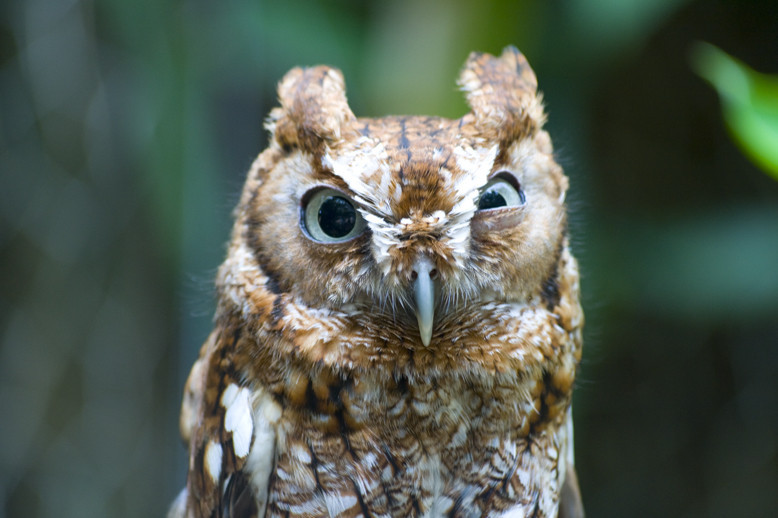
\includegraphics[width= 0.6 \textwidth]{./Figs/placeholder.jpeg}  
    \caption{Likelihood profile for \tmumu.}
    \label{fig:taulike}
\end{figure}

\begin{figure}[htbp]
    \centering
   \begin{subfigure}[b]{0.48\textwidth}
        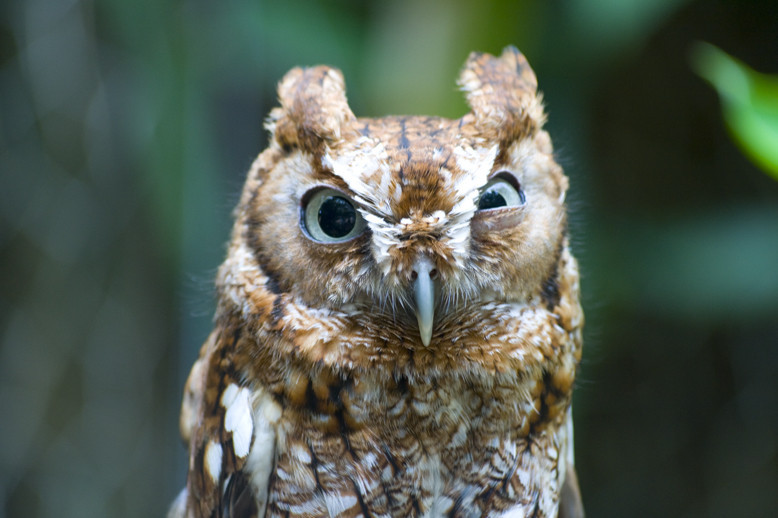
\includegraphics[width= \textwidth]{./Figs/placeholder.jpeg}
        %\caption{ }                                                                                                                    
        %\label{fig:BDTSsig}                                                                                                            
    \end{subfigure}
   ~ %add desired spacing between images, e. g. ~, \quad, \qquad, \hfill etc.                                                         
      %(or a blank line to force the subfigure onto a new line)                                                                         
    \begin{subfigure}[b]{0.48\textwidth}
       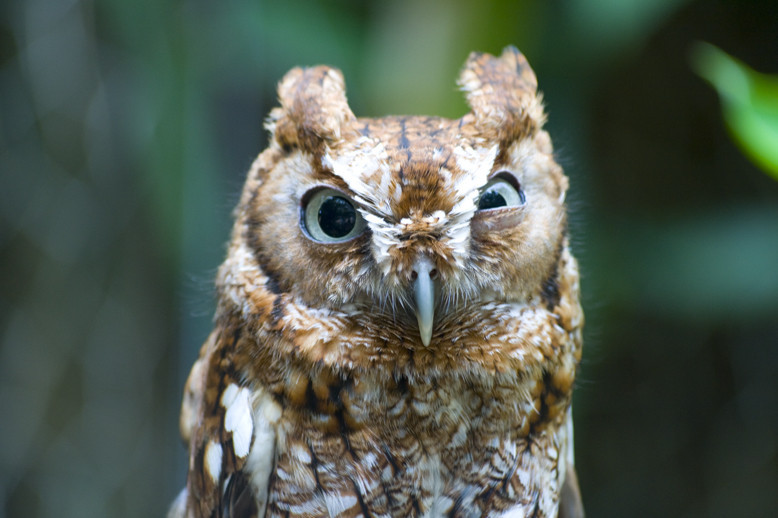
\includegraphics[width=\textwidth]{./Figs/placeholder.jpeg}
      %  \caption{ }                                                                                                                    
     %   \label{fig:BDTSbkg}                                                                                                            
   \end{subfigure}
    \caption{Pull distribution for \tmumu using simplified toys for 50 and 300 \fb.}
    \label{fig:morestatstaupulls}
\end{figure}


The bias in the \tmumu pull distribution shows that the distribution cannot be interpreted in the usually way and also that the statistical uncertainties from the \ml to the weighted decay time distribution may not be correct. 

However another way to assess the accuracy of the statistical uncertainties returned by the \ml fit is the coverage of the uncertainties; the percentage of fitted values of \tmumu from the toy studies that fall within 1, 2 and 3 standard deviations of the input lifetime used to generate the \bsmumu decay time distribution. Table~\ref{tab:LifetimeCoverage} shows the coverage of the statistical uncertainties for \tmumu for 10,000 toy studies for the expected \bsmumu and combinatorial background yields alongside the intervals expected for a Gaussian distribution. A comparison between the coverage of \tmumu and the Gaussian intervals shows that the coverage of the statistical uncertainties is very close to the expected coverage, therefore with the expected statistic fitting for \tmumu would be appropriate.

{\it I don't think that I really understand this and I probably should, it would help with the writing!}
\begin{table}[ht]
\begin{center}
\begin{tabular}{lccc}
\hline
 & \tmumu &  \Gmumu & Gaussian \\ \hline 
$1\sigma$ & 68.52$\%$ & 68.67$\%$ & 68.27$\%$ \\
$2\sigma$ &  93.82$\%$ & 95.29$\%$ &  95.45 $\%$ \\
$3\sigma$ & 98.54$\%$ &  99.66$\%$ & 99.73 $\%$ \\ \hline
\end{tabular}
\caption{Coverage.}
\label{tab:LifetimeCoverage}
\end{center}
\end{table}

Alternatively, a way to get around having a biased pull distribution is to measure the inverse of the effective lifetime, \invtmumu$ \equiv$ \Gmumu. The pull distributions for \Gmumu are shown in Figure~\ref{fig:gammapulls} and produce unbiased pull values regardless of the statistics. This is unsurprising given the smooth log-likelihood profile as a function of \Gmumu shown in Figure~\ref{fig:gammalike}. Furthermore the statistical coverage of \Gmumu is even closer to the Gaussian intervals than that of \tmumu.


\begin{figure}[htbp]
    \centering
        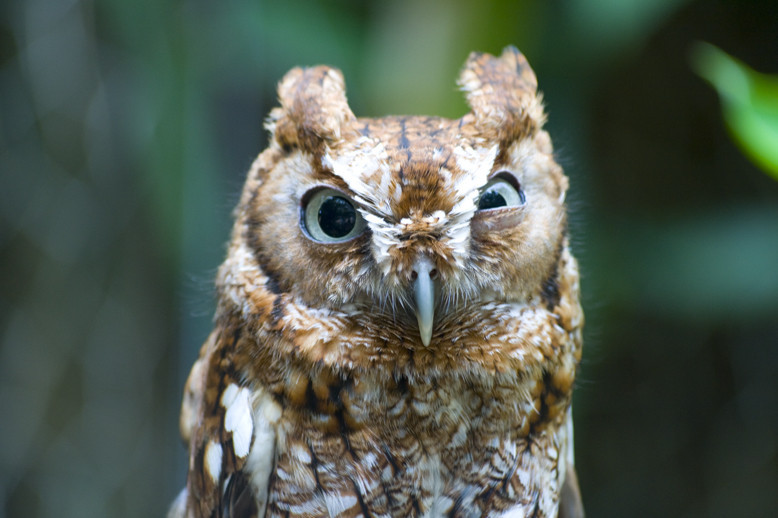
\includegraphics[width= 0.6 \textwidth]{./Figs/placeholder.jpeg}  
    \caption{Likelihood profile for \Gmumu.}
    \label{fig:gammalike}
\end{figure}

\begin{figure}[htbp]
    \centering
  \begin{subfigure}[b]{0.6\textwidth}
        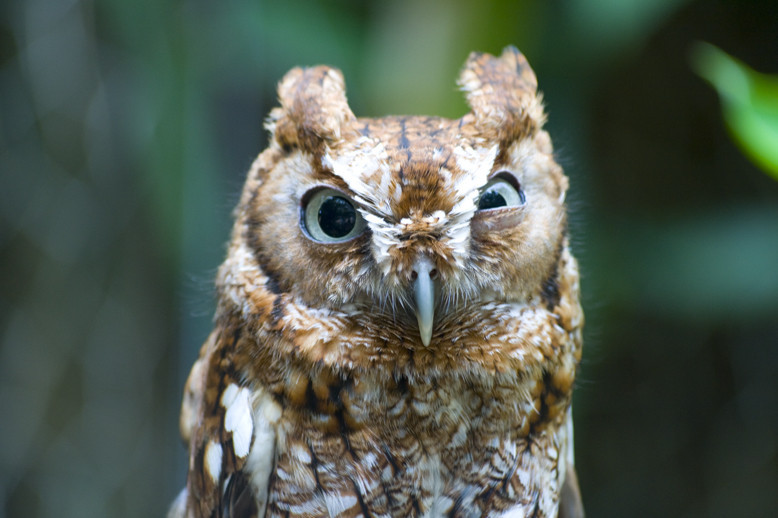
\includegraphics[width= \textwidth]{./Figs/placeholder.jpeg}
        %\caption{ }                                                                                                                    
        %\label{fig:BDTSsig}                                                                                                            
    \end{subfigure}


   \begin{subfigure}[b]{0.48\textwidth}
        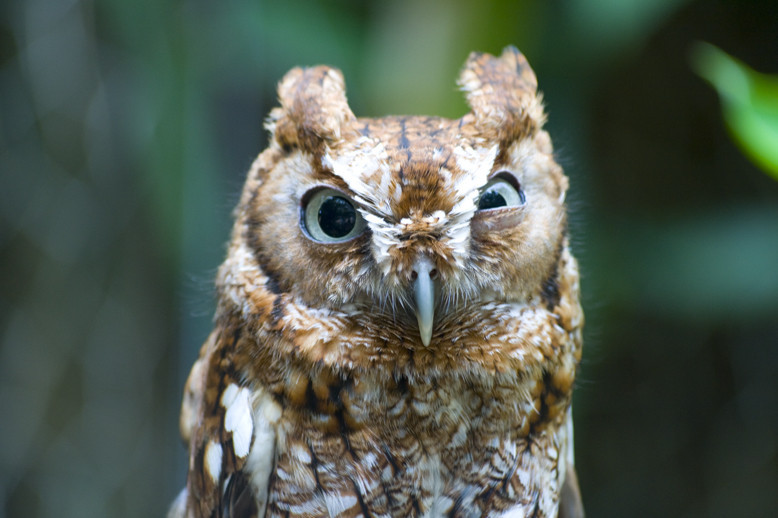
\includegraphics[width= \textwidth]{./Figs/placeholder.jpeg}
        %\caption{ }                                                                                                                    
        %\label{fig:BDTSsig}                                                                                                            
    \end{subfigure}
   ~ %add desired spacing between images, e. g. ~, \quad, \qquad, \hfill etc.                                                         
      %(or a blank line to force the subfigure onto a new line)                                                                         
    \begin{subfigure}[b]{0.48\textwidth}
       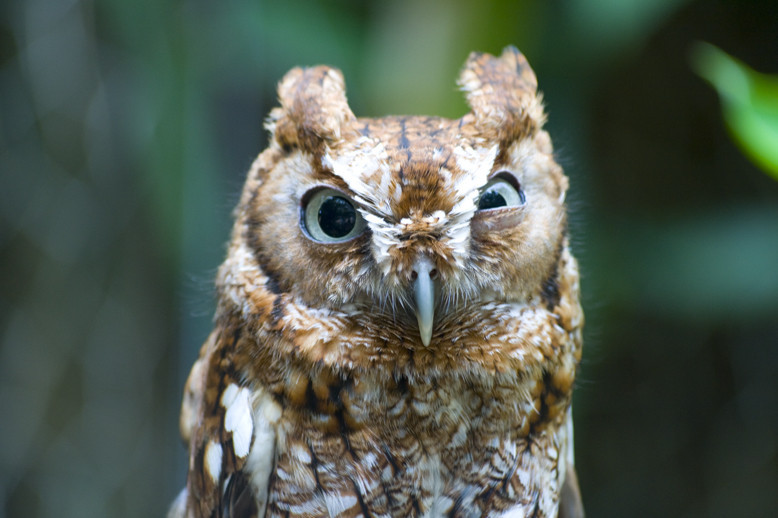
\includegraphics[width=\textwidth]{./Figs/placeholder.jpeg}
      %  \caption{ }                                                                                                                    
     %   \label{fig:BDTSbkg}                                                                                                            
   \end{subfigure}
    \caption{Pull distribution for \Gmumu using simplified toys for 4.4, 50 and 300 \fb.}
    \label{fig:gammapulls}
\end{figure}



 However the lifetime is a more interesting variable from a physics point of view due to its relationship with \ADG. Furthermore fitting for the \Gmumu introduces a different type of bias in to the fit, but this is negligible for the expected number of statistics. 



Ideally the fit strategy would be performed to extract the lifetime not the inverse lifetime, however for the moment the \ml fit for both \tmumu and \Gmumu will be used in the toy studies. The statistical coverage for both parameters is good and using either is reasonable. The final decision will be made based on the statistical coverage expected for the observed number of decays in the data set. 

%Perhaps the order could be
%- Pulls are biased for the lifetime
%- likelihood shows that the problem could be in the error, so can we trust it
%- coverage shows that it's good enough to use
%- alternatively could fit for the inverse, this has good pulls, expected from the likelihood and also look good coverage
%- however inv lifetime has a different bias
%- ideally want to fit the lifetime
%- look at both for now, final decision will be made later
%- biases from the fit as discussed futher in the next chapter

   
\subsection{Toy Results}
\label{sec:toyresults}

%Plan
% - looked at different mass configurations, these are ....
% - Ran 10,000 toys for each configuration
% - All backgrounds are generated regardless of what is included into the fit
% - The results are shown in Table X for the different options
% - The conclusions is to use this configuration, hence the mass cut described in the selection Chapter
% - This is what we expect the fit to look like
% - The expected uncertainties are shown here, there is a large range so realisatically could be between 0.1 and 0.8ps or the other for inv lifetime
% - Prehaps the full details of the pdfs used are given in the appendix?
% - I could add some pulls or plots of othe examples?
% - Do I actually need to show all the results or not? I could just say in words that we looked at various things and we deceided the following?? Also how do I say this work - is it mine of Harry's or is it a collaboration?
Different mass ranges, and consequently backgrounds included in the \ml fit, are tested through the toy studies to determine configuration that produces the smallest expected uncertainty on the measurement of \tmumu and \Gmumu.
The mass distribution of expected number \bsmumu candidates passing the effective lifetime selection is shown in Figure~\ref{} assuming the Standard Model \bmumu branching fractions. The contributions from each source are overlaid. The backgrounds beneath the \bs mass peak are the combinatorial background and the high mass tails of the \bhh, \bdmum and \lambdab backgrounds. The mass distribution in Figure~\ref{} is used to chose the different mass \pdfs.

In each fit configuration the mass \pdf has the form
\begin{equation}
PDF(m) = \displaystyle\sum_{i} N^{Bk}_{i}PDF^{Bk}_{i}(m) + N^{B^{0}_{s} \to \mu^{+} \mu^{-}}PDF^{B^{0}_{s} \to \mu^{+} \mu^{-}}(m)
\end{equation}
where $N$ and $PDF$ are the yields and \pdfs of the signal (backgrounds) in the fit. The mass ranges and backgrounds included in the \pdf for the different configurations are;


For each possible mass fit configuration the \bsmumu and combinatorial background yields are let free in the fit where as the yield of any other backgrounds are constrained to their expected values in the fit. Also all mass shapes are fixed in the \ml fit except the slope of the combinatorial background because this is not accurately known.
The SM prediction for the \bsmumu effective lifetime is used to generate events for the toy studies and regardless of which background components are included in the mass fit all backgrounds are generated for each mass range. 

A total of X toy studies are performed for each mass fit range and the results are given in Table~\ref{}. The mean and widths of \Gmumu, the \bsmumu yield and combinatorial background yield and slope as well as the median expected uncertainty on \tmumu and \Gmumu are used to measure the performance of each mass fit configuration. The pull distribution of the fit for \tmumu is not used to assess the performance of each mass fit confirmation given the discussion in Section~\ref{}.

Figure~\ref{fig:toygen} shows the generated mass and decay time distributions for the mass range 4900 - 6000 and Figure~\ref{fig:toyegs} gives examples of the mass and decay time distributions and \ml fit for a selection of mass fit configurations. 

\begin{figure}[htbp]
    \centering
   \begin{subfigure}[b]{0.48\textwidth}
        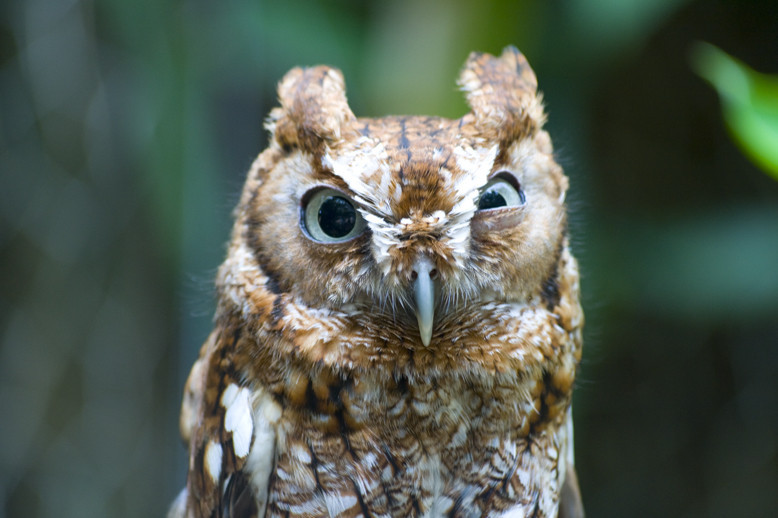
\includegraphics[width= \textwidth]{./Figs/placeholder.jpeg}
        %\caption{ }                                                                                                                    
        %\label{fig:BDTSsig}                                                                                                            
    \end{subfigure}
   ~ %add desired spacing between images, e. g. ~, \quad, \qquad, \hfill etc.                                                         
      %(or a blank line to force the subfigure onto a new line)                                                                         
    \begin{subfigure}[b]{0.48\textwidth}
       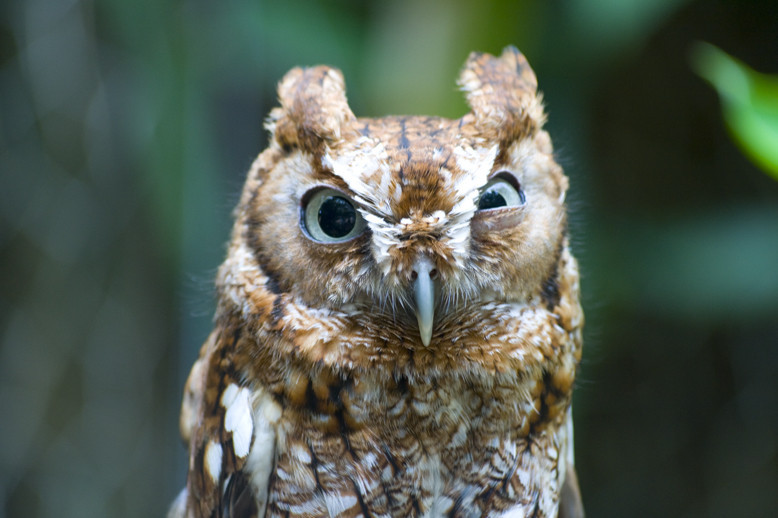
\includegraphics[width=\textwidth]{./Figs/placeholder.jpeg}
      %  \caption{ }                                                                                                                    
     %   \label{fig:BDTSbkg}                                                                                                            
   \end{subfigure}
    \caption{Mass and decay time distributions for the generated decays in the mass range 4900 - 6000.}
    \label{fig:toygen}
\end{figure}

\begin{figure}[htbp]
    \centering
   \begin{subfigure}[b]{0.48\textwidth}
        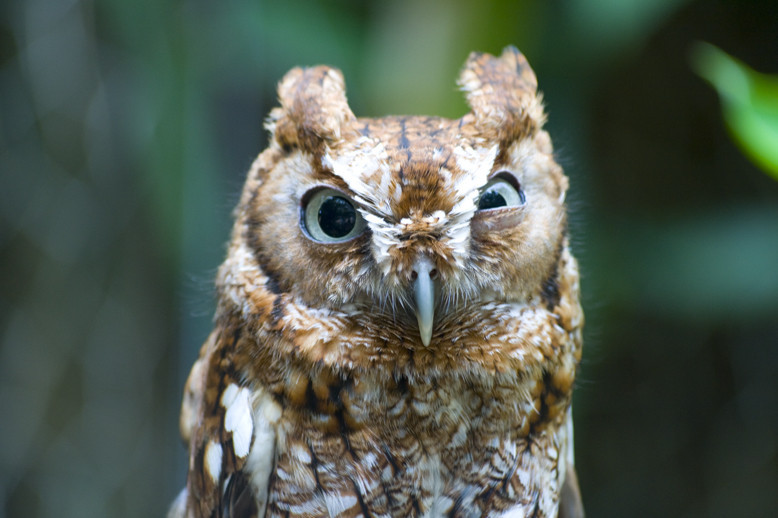
\includegraphics[width= \textwidth]{./Figs/placeholder.jpeg}
        %\caption{ }                                                                                                                    
        %\label{fig:BDTSsig}                                                                                                            
    \end{subfigure}
   ~ %add desired spacing between images, e. g. ~, \quad, \qquad, \hfill etc.                                                         
      %(or a blank line to force the subfigure onto a new line)                                                                         
    \begin{subfigure}[b]{0.48\textwidth}
       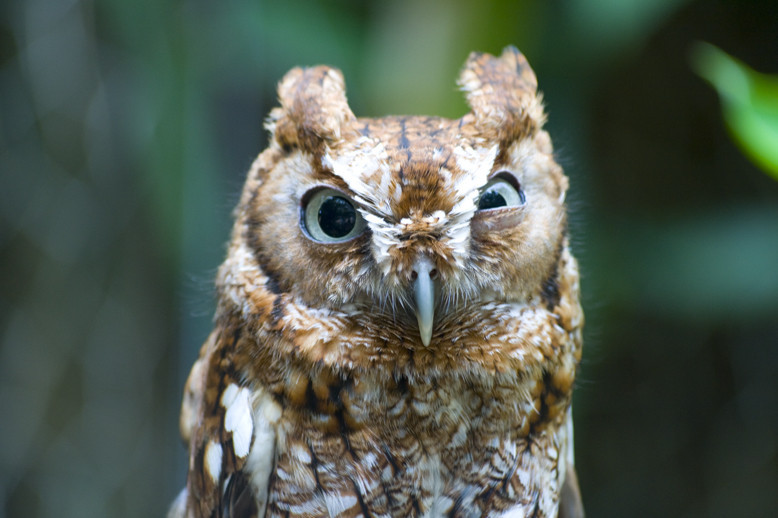
\includegraphics[width=\textwidth]{./Figs/placeholder.jpeg}
      %  \caption{ }                                                                                                                    
     %   \label{fig:BDTSbkg}                                                                                                            
   \end{subfigure}


  \begin{subfigure}[b]{0.48\textwidth}
        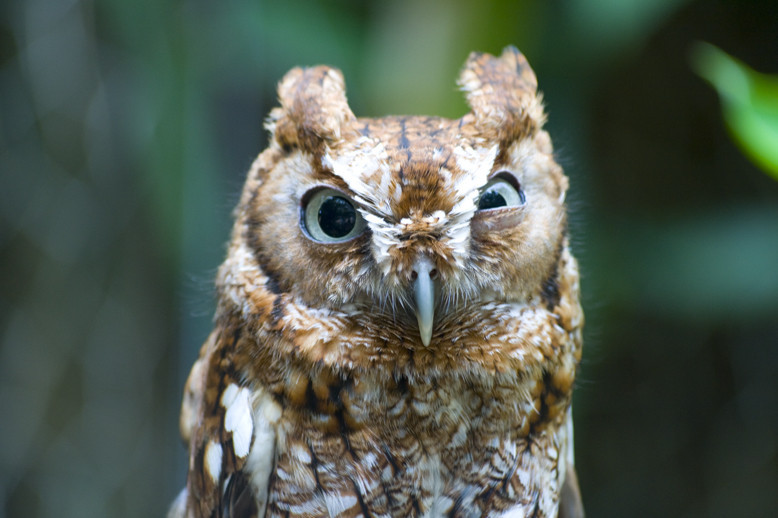
\includegraphics[width= \textwidth]{./Figs/placeholder.jpeg}
        %\caption{ }                                                                                                                    
        %\label{fig:BDTSsig}                                                                                                            
    \end{subfigure}
   ~ %add desired spacing between images, e. g. ~, \quad, \qquad, \hfill etc.                                                         
      %(or a blank line to force the subfigure onto a new line)                                                                         
    \begin{subfigure}[b]{0.48\textwidth}
       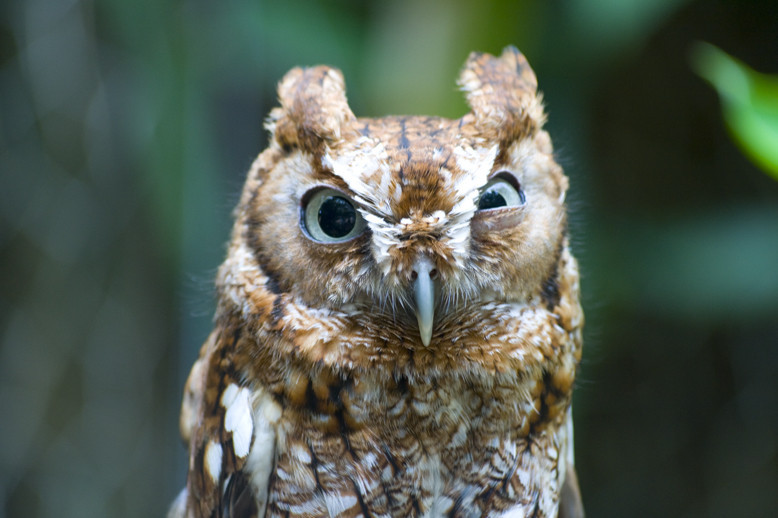
\includegraphics[width=\textwidth]{./Figs/placeholder.jpeg}
      %  \caption{ }                                                                                                                    
     %   \label{fig:BDTSbkg}                                                                                                            
   \end{subfigure}


  \begin{subfigure}[b]{0.48\textwidth}
        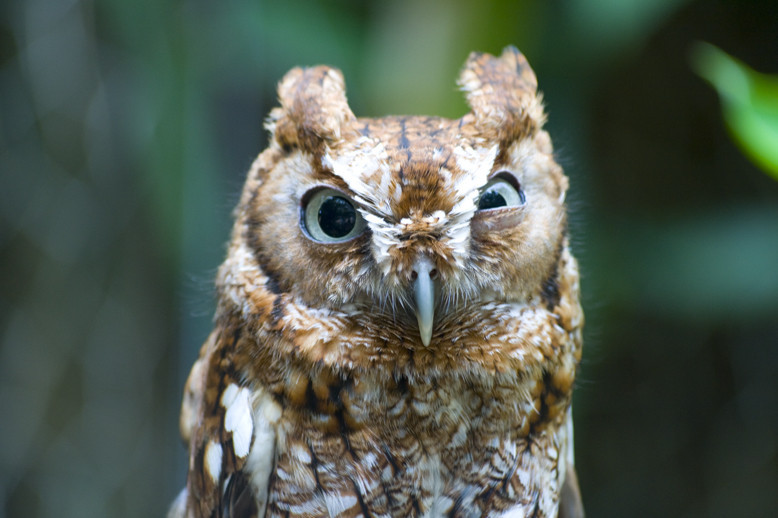
\includegraphics[width= \textwidth]{./Figs/placeholder.jpeg}
        %\caption{ }                                                                                                                    
        %\label{fig:BDTSsig}                                                                                                            
    \end{subfigure}
   ~ %add desired spacing between images, e. g. ~, \quad, \qquad, \hfill etc.                                                         
      %(or a blank line to force the subfigure onto a new line)                                                                         
    \begin{subfigure}[b]{0.48\textwidth}
       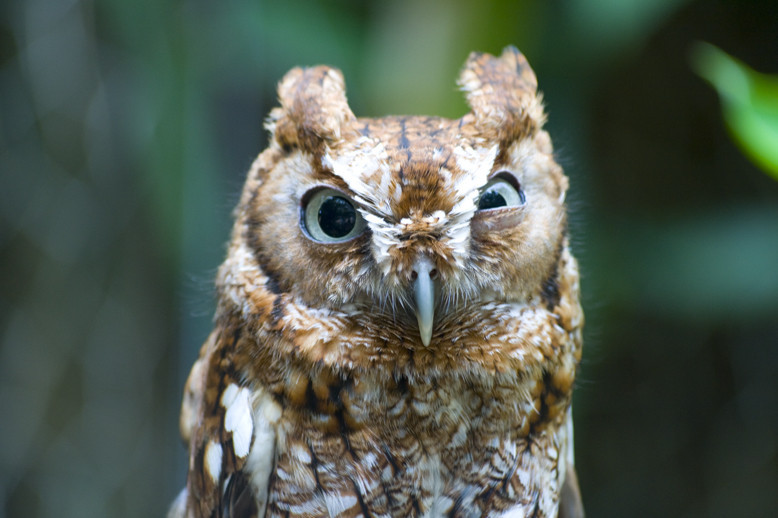
\includegraphics[width=\textwidth]{./Figs/placeholder.jpeg}
      %  \caption{ }                                                                                                                    
     %   \label{fig:BDTSbkg}                                                                                                            
   \end{subfigure}


    \caption{Mass and decay time \ml fit for toy configurations X, Y and Z.}
    \label{fig:toyegs}
\end{figure}


The expected uncertainties for \tmumu and \Gmumu are smallest for mass of the simplest mass fit configuration, fit number X, where the mass range is restricted to 5320 - 6000 \mevcc and only the \bsmumu and combinatorial background components are used in the total mass \pdf. The mean and widths for the different pull distributions are consistent with the expected mean of 0 and width of 1 for this fit configuration. The wider mass ranges with more background components in the mass \pdf have much larger expected uncertainties for \tmumu and \Gmumu as well as clearly biased pull distributions. It is not surprising that the simplest fit performs the best given the very low expected number of events. 

Therefore the fit configuration number X is chosen to measure the \bsmumu effective lifetime (or its inverse). From Figure~\ref{} it is clear that the number of background decays from \bdmumu, \bhh and \lambdab is extremely mass above 5320 \mevcc therefore these backgrounds do not need to be modelled in the mass \pdf. The affect on the final result of not modelling these backgrounds is estimated in Section~\ref{}. The mean and widths for the different pull distributions are consistent with the expected mean of 0 and width of 1. 


The expected uncertainties for the chosen fit configuration for \tmumu and \Gmumu are X and Y. However due to the low expected number of decays there is a large spread in the expected uncertainties as shown in Figure~\ref{}. Therefore the uncertainties on the measurements would range between X and Y for \tmumu and P and O for \Gmumu.


\section{Results}
\label{sec:ELresults}

The results of the unbinned \ml fit to the dimuon mass distribution and the sWeighted decay time of \bsmumu candidates for 4.4~\fb of Run 1 and Run 2 data are shown in Figure~\ref{fig:ELresults}, 22 $\pm$ 6 \bsmumu decays were observed and 20 $\pm$ 6 combinatorial background decays. The measured values of \tmumu and \Gmumu are
\begin{equation}
\tau_{\mu\mu} = 2.04 \pm 0.44 \pm 0.05 \text{ps} 
\end{equation}
\begin{equation}
\Gamma_{\mu\mu} = 0.489  \pm 0.117  \pm  0.014 \text{ps}
\end{equation}

where the uncertainties are only statistical. The results are consistent with the SM prediction of \tmumu = \tH within  1 $\sigma$ and within  1.5 $\sigma$ of \tmumu = \tL.

The observed number of decays is lower than expected and the statistical coverage of the uncertainties has been checked using toy studies generated with the observed number of decays. In the toy studies the background decays from \bhh, \bdmumu and \lambdab are included at the expected level. The coverage of both \tmumu and \Gmumu statistical uncertainties is good, as shown in Table~\ref{tab:LifetimeCoverage_observed}, therefore given the observed number of decays the result of the more inter sting \tmumu and its statistical uncertainty can be trusted as accurate. %The bias introduced by the fit strategy is estimated in Chapter X. 



\begin{figure}[htbp]
    \centering
   \begin{subfigure}[b]{0.48\textwidth}
        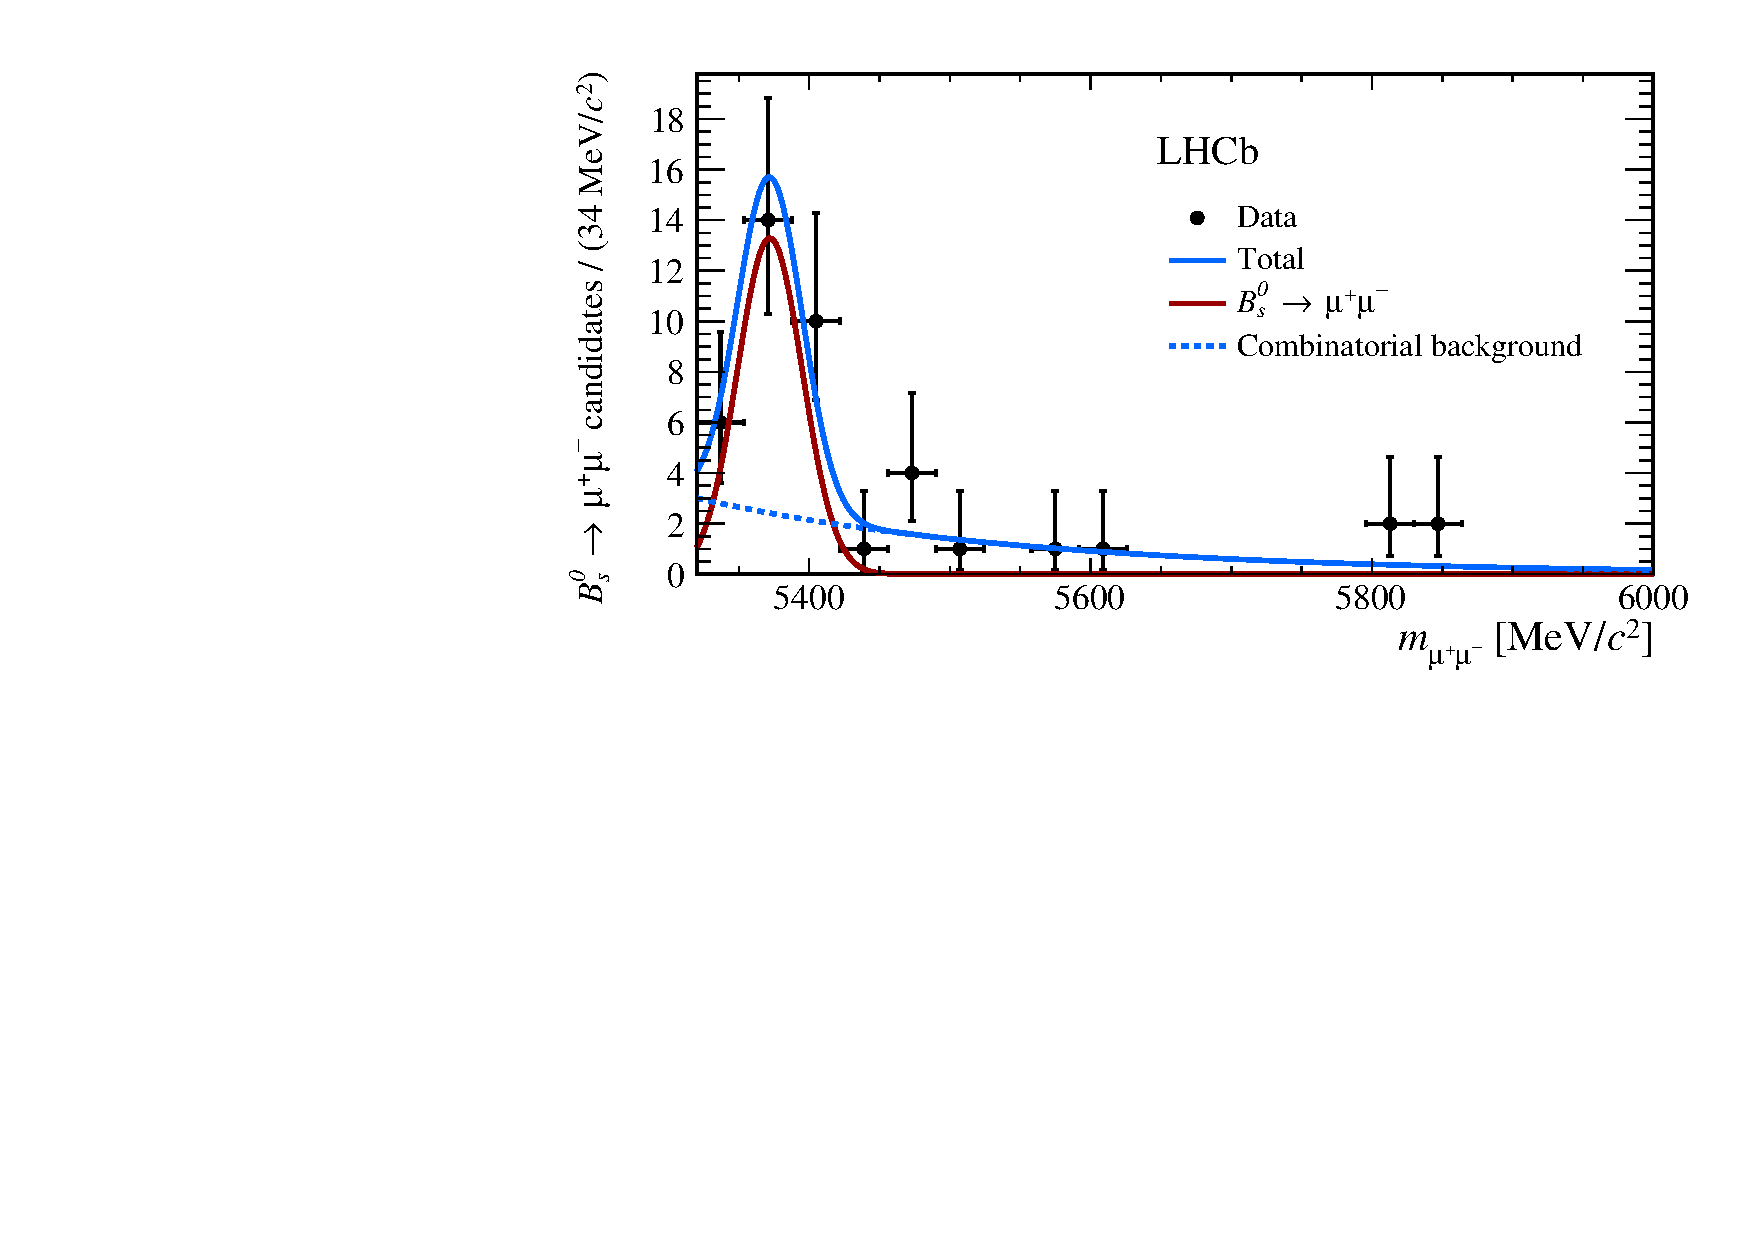
\includegraphics[width= \textwidth]{./Figs/LifetimeMeasurement/mass_fit_lifetime.pdf}
        %\caption{ }                                                                                                                    
        %\label{fig:BDTSsig}                                                                                                            
    \end{subfigure}
   ~ %add desired spacing between images, e. g. ~, \quad, \qquad, \hfill etc.                                                         
      %(or a blank line to force the subfigure onto a new line)                                                                         
    \begin{subfigure}[b]{0.48\textwidth}
       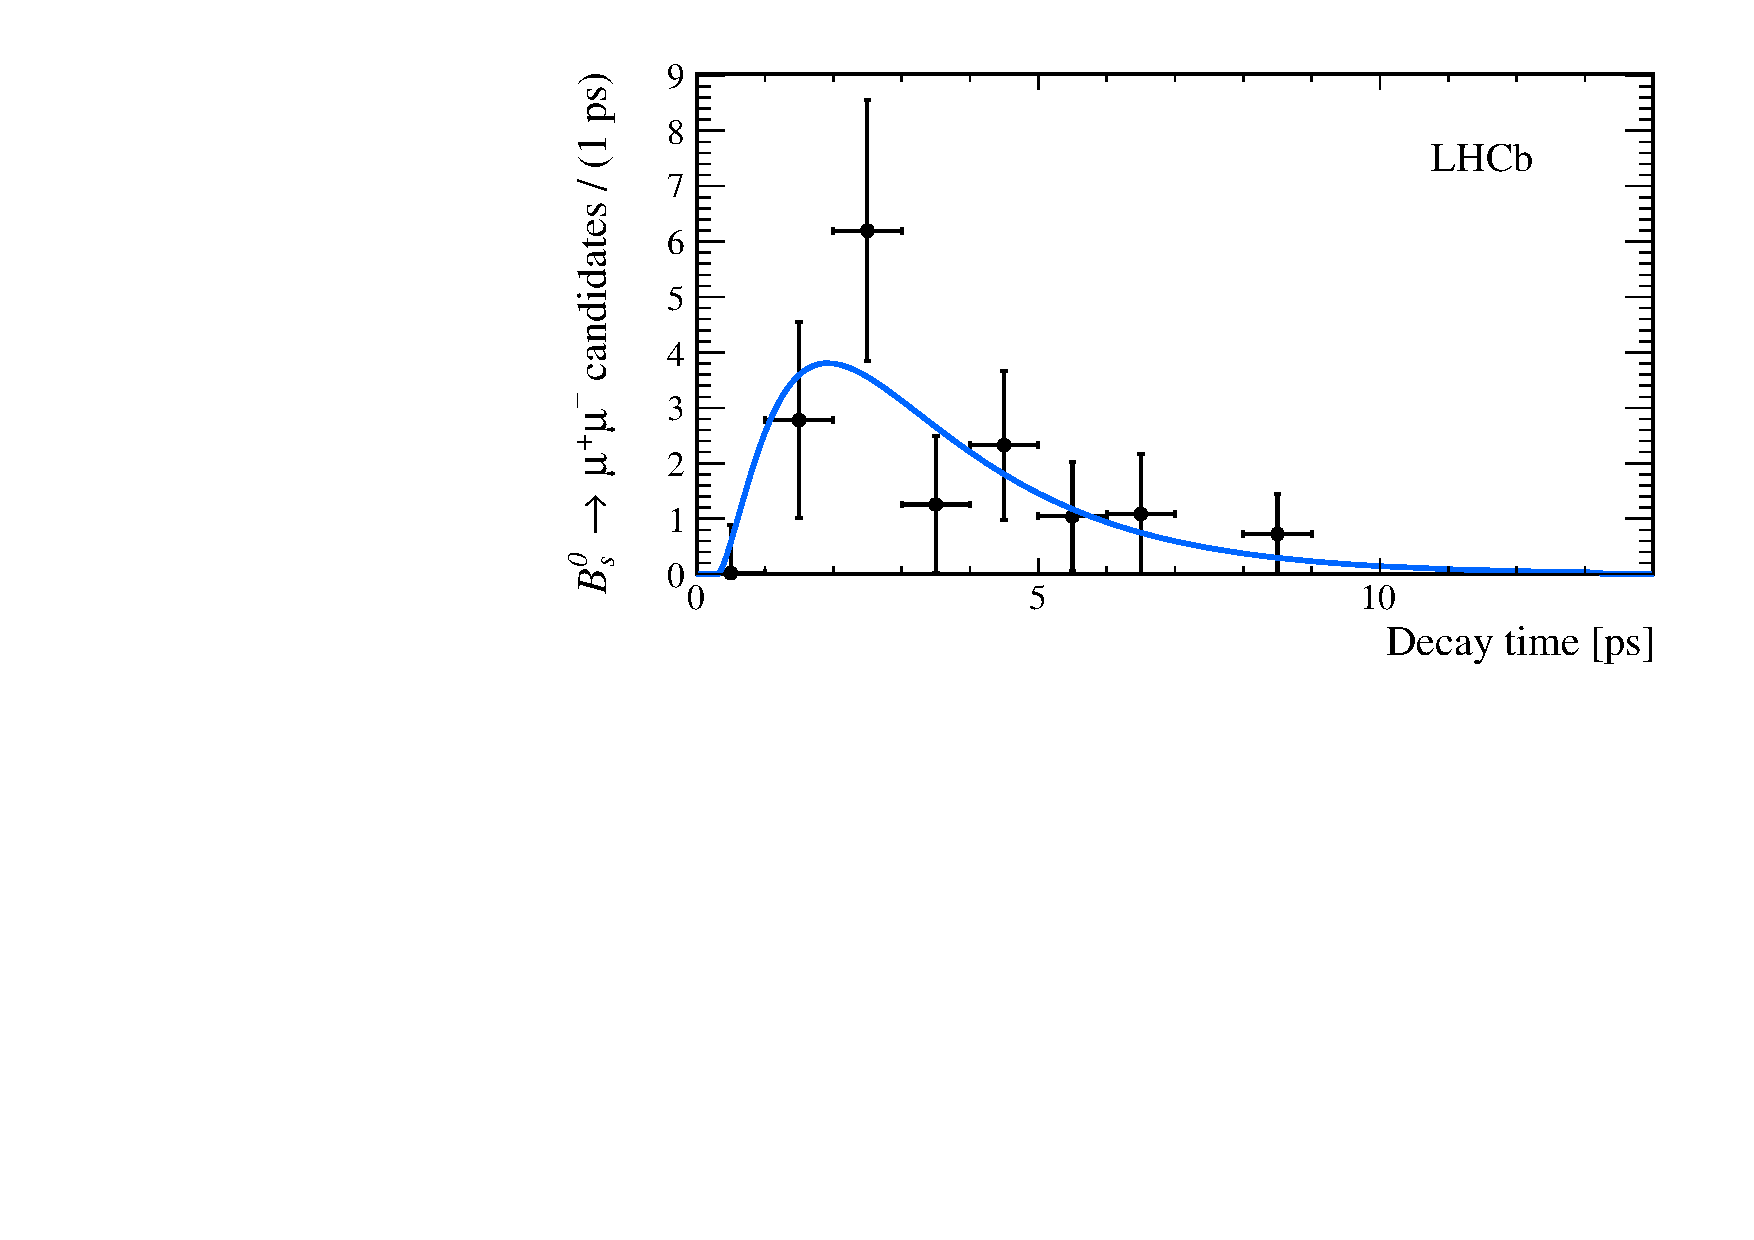
\includegraphics[width=\textwidth]{./Figs/LifetimeMeasurement/lifetime_fit.pdf}
      %  \caption{ }                                                                                                                    
     %   \label{fig:BDTSbkg}                                                                                                            
   \end{subfigure}
    \caption{Maximum likelihood fit to the invariant mass distribution (left) and weighted decay time distribution (right) of \bsmumu candidates in 4.4 \fb of data collected by the LHCb experiment. \bsmumu candidates are described by the red peak in the mass plot and combinatorial background by the blue dashed line, the total \pdf is given by the solid blue line.}
    \label{fig:ELresults}
\end{figure}


\begin{table}[ht]
\begin{center}
\begin{tabular}{lccc}
\hline
 & \tmumu &  \Gmumu & Gaussian \\ \hline 
$1\sigma$ & 68.83\% & 67.76\% & 68.27\% \\
$2\sigma$ &  93.11\% & 95.55\% &  95.45 \% \\
$3\sigma$ & 97.92\% &  99.67\% & 99.73 \% \\ \hline
\end{tabular}
\caption{Coverage of observed decays.}
\label{tab:LifetimeCoverage_observed}
\end{center}
\end{table}
